%%%%%%%%%%%%%%%%%%%%%%%%%%%%%%%%%%%%%%%%%%%%%%%%%%%%%%%%%%%%%%%
%% OXFORD THESIS TEMPLATE

% Use this template to produce a standard thesis that meets the Oxford University requirements for DPhil submission
%
% Originally by Keith A. Gillow (gillow@maths.ox.ac.uk), 1997
% Modified by Sam Evans (sam@samuelevansresearch.org), 2007
% Modified by John McManigle (john@oxfordechoes.com), 2015
%
% This version Copyright (c) 2015-2017 John McManigle
%
% Broad permissions are granted to use, modify, and distribute this software
% as specified in the MIT License included in this distribution's LICENSE file.
%

% I've (John) tried to comment this file extensively, so read through it to see how to use the various options.  Remember
% that in LaTeX, any line starting with a % is NOT executed.  Several places below, you have a choice of which line to use
% out of multiple options (eg draft vs final, for PDF vs for binding, etc.)  When you pick one, add a % to the beginning of
% the lines you don't want.


%%%%% CHOOSE PAGE LAYOUT
% The most common choices should be below.  You can also do other things, like replacing "a4paper" with "letterpaper", etc.

% This one will format for two-sided binding (ie left and right pages have mirror margins; blank pages inserted where needed):
\documentclass[a4paper,twoside]{ociamthesis}
% This one will format for one-sided binding (ie left margin > right margin; no extra blank pages):
%\documentclass[a4paper]{ociamthesis}
% This one will format for PDF output (ie equal margins, no extra blank pages):
%\documentclass[a4paper,nobind]{ociamthesis} 



%%%%% SELECT YOUR DRAFT OPTIONS
% Three options going on here; use in any combination.  But remember to turn the first two off before
% generating a PDF to send to the printer!

% This adds a "DRAFT" footer to every normal page.  (The first page of each chapter is not a "normal" page.)
\fancyfoot[C]{\emph{DRAFT Printed on \today}}  

% This highlights (in blue) corrections marked with (for words) \mccorrect{blah} or (for whole
% paragraphs) \begin{mccorrection} . . . \end{mccorrection}.  This can be useful for sending a PDF of
% your corrected thesis to your examiners for review.  Turn it off, and the blue disappears.
\correctionstrue


%%%%% BIBLIOGRAPHY SETUP
% Note that your bibliography will require some tweaking depending on your department, preferred format, etc.
% The options included below are just very basic "sciencey" and "humanitiesey" options to get started.
% If you've not used LaTeX before, I recommend reading a little about biblatex/biber and getting started with it.
% If you're already a LaTeX pro and are used to natbib or something, modify as necessary.
% Either way, you'll have to choose and configure an appropriate bibliography format...

% The science-type option: numerical in-text citation with references in order of appearance.
\usepackage[style=numeric-comp, sorting=none, backend=biber, doi=false, isbn=false, url=false, arxiv=false]{biblatex}
\newcommand*{\bibtitle}{References}

% The humanities-type option: author-year in-text citation with an alphabetical works cited.
%\usepackage[style=authoryear, sorting=nyt, backend=biber, maxcitenames=2, useprefix, doi=false, isbn=false]{biblatex}
%\newcommand*{\bibtitle}{Works Cited}

% This makes the bibliography left-aligned (not 'justified') and slightly smaller font.
\renewcommand*{\bibfont}{\raggedright\small}

% Change this to the name of your .bib file (usually exported from a citation manager like Zotero or EndNote).
\addbibresource{references.bib}


% Uncomment this if you want equation numbers per section (2.3.12), instead of per chapter (2.18):
%\numberwithin{equation}{subsection}



%%%%% THESIS / TITLE PAGE INFORMATION
% Everybody needs to complete the following:
\title{Rings and Things}
\author{David Ormrod Morley}
\college{Balliol College}

% Master's candidates who require the alternate title page (with candidate number and word count)
% must also un-comment and complete the following three lines:
%\masterssubmissiontrue
%\candidateno{933516}
%\wordcount{28,815}

% Uncomment the following line if your degree also includes exams (eg most masters):
%\renewcommand{\submittedtext}{Submitted in partial completion of the}
% Your full degree name.  (But remember that DPhils aren't "in" anything.  They're just DPhils.)
\degree{Doctor of Philosophy}
% Term and year of submission, or date if your board requires (eg most masters)
\degreedate{Trinity 2020}


%%%%% YOUR OWN PERSONAL MACROS
% This is a good place to dump your own LaTeX macros as they come up.

% To make text superscripts shortcuts
	\renewcommand{\th}{\textsuperscript{th}} % ex: I won 4\th place
	\newcommand{\nd}{\textsuperscript{nd}}
	\renewcommand{\st}{\textsuperscript{st}}
	\newcommand{\rd}{\textsuperscript{rd}}

%%%%% THE ACTUAL DOCUMENT STARTS HERE
\begin{document}



%%%%% CHOOSE YOUR LINE SPACING HERE
% This is the official option.  Use it for your submission copy and library copy:
\setlength{\textbaselineskip}{22pt plus2pt}
% This is closer spacing (about 1.5-spaced) that you might prefer for your personal copies:
%\setlength{\textbaselineskip}{18pt plus2pt minus1pt}

% You can set the spacing here for the roman-numbered pages (acknowledgements, table of contents, etc.)
\setlength{\frontmatterbaselineskip}{17pt plus1pt minus1pt}

% Leave this line alone; it gets things started for the real document.
\setlength{\baselineskip}{\textbaselineskip}


%%%%% CHOOSE YOUR SECTION NUMBERING DEPTH HERE
% You have two choices.  First, how far down are sections numbered?  (Below that, they're named but
% don't get numbers.)  Second, what level of section appears in the table of contents?  These don't have
% to match: you can have numbered sections that don't show up in the ToC, or unnumbered sections that
% do.  Throughout, 0 = chapter; 1 = section; 2 = subsection; 3 = subsubsection, 4 = paragraph...

% The level that gets a number:
\setcounter{secnumdepth}{2}
% The level that shows up in the ToC:
\setcounter{tocdepth}{2}


%%%%% ABSTRACT SEPARATE
% This is used to create the separate, one-page abstract that you are required to hand into the Exam
% Schools.  You can comment it out to generate a PDF for printing or whatnot.
%\begin{abstractseparate}
%	Investigations into \td{} network\--forming materials have renewed importance due to the experimental synthesis of ultra\--thin films of carbon, silica and aluminosilicate glasses.
Microscopy on the disordered phases of these materials reveals a percolating ring structure, identifying them as candidates for range of technologically useful materials, with applications including catalysis and gas separation.
The ability to characterise, understand and control the structure of the pore landscape in such materials is therefore central to their further development.

The overall aim of this thesis is to improve the simulation and characterisation of \td{} disordered materials.
The key is to accurately quantify and reproduce the ring structure, described by the ring size distribution and ring\--ring correlations.
This will be achieved by relating previous empirical laws (namely \lm's law and the \aw{} law), to well\--defined metrics in network science, and developing a variety of \mc{} methods to generate networks with controllable ring structure and topologies.

The first of these methods will be a sequential growth algorithm to construct triangle rafts (a proxy for silica bilayers), which will be shown to produce configurations commensurate with those from experiment.
Following from this, a modified bond switching algorithm will be used to investigate more generic systems, spanning a variety of atomic coordination environments, potential models and topologies. 
Fundamental relationships between these measures and the ring structure will be demonstrated by systematically varying the system parameters.
In addition, hard particle \mc{} techniques will be used to generate Voronoi diagrams, making contact with experimental studies on quasi\--\td{} colloidal systems.

Treating these diverse physical systems as complex networks allows a generalised network theory to be developed.
Traditional ring measures will be related to well\--defined metrics from network theory, namely the node degree distribution and the assortativity.
This will enable seemingly disparate physical systems to be compared and ties them into the wider field of network science.

Further applications of this work to real systems will be illustrated with analyses on a range of experimental (or experimentally motivated) data.
The appropriateness of weighted and unweighted Voronoi constructions will be evaluated for colloidal monolayers.
The ring structure of procrystalline lattices will be demonstrated to be related to the underlying parent lattice and atomic coordination environments.
Finally, a tool from topological data analysis, termed persistent homology, will be investigated and shown to be a potential complement to more traditional measures of structural disorder.

%\textbf{Keywords}: Network theory, Monte Carlo methods, silica bilayers, colloidal monolayers, procrystalline lattices, Voronoi diagrams, persistent homology
 % Create an abstract.tex file in the 'text' folder for your abstract.
%\end{abstractseparate}


% JEM: Pages are roman numbered from here, though page numbers are invisible until ToC.  This is in
% keeping with most typesetting conventions.
\begin{romanpages}

% Title page is created here
\maketitle

%%%%% DEDICATION -- If you'd like one, un-comment the following.
%\begin{dedication}
%This thesis is dedicated to\\
%someone\\
%for some special reason\\
%\end{dedication}

%%%%% ACKNOWLEDGEMENTS -- Nothing to do here except comment out if you don't want it.
%\begin{acknowledgements}
% 	%\subsection*{Personal}

So long, and thanks for all the fish.

%\subsection*{Institutional}

%If you want to separate out your thanks for funding and institutional support, I don't think there's any rule against it.  Of course, you could also just remove the subsections and do one big traditional acknowledgement section.

%\end{acknowledgements}

%%%%% ABSTRACT -- Nothing to do here except comment out if you don't want it.
%\begin{abstract}
%	Investigations into \td{} network\--forming materials have renewed importance due to the experimental synthesis of ultra\--thin films of carbon, silica and aluminosilicate glasses.
Microscopy on the disordered phases of these materials reveals a percolating ring structure, identifying them as candidates for range of technologically useful materials, with applications including catalysis and gas separation.
The ability to characterise, understand and control the structure of the pore landscape in such materials is therefore central to their further development.

The overall aim of this thesis is to improve the simulation and characterisation of \td{} disordered materials.
The key is to accurately quantify and reproduce the ring structure, described by the ring size distribution and ring\--ring correlations.
This will be achieved by relating previous empirical laws (namely \lm's law and the \aw{} law), to well\--defined metrics in network science, and developing a variety of \mc{} methods to generate networks with controllable ring structure and topologies.

The first of these methods will be a sequential growth algorithm to construct triangle rafts (a proxy for silica bilayers), which will be shown to produce configurations commensurate with those from experiment.
Following from this, a modified bond switching algorithm will be used to investigate more generic systems, spanning a variety of atomic coordination environments, potential models and topologies. 
Fundamental relationships between these measures and the ring structure will be demonstrated by systematically varying the system parameters.
In addition, hard particle \mc{} techniques will be used to generate Voronoi diagrams, making contact with experimental studies on quasi\--\td{} colloidal systems.

Treating these diverse physical systems as complex networks allows a generalised network theory to be developed.
Traditional ring measures will be related to well\--defined metrics from network theory, namely the node degree distribution and the assortativity.
This will enable seemingly disparate physical systems to be compared and ties them into the wider field of network science.

Further applications of this work to real systems will be illustrated with analyses on a range of experimental (or experimentally motivated) data.
The appropriateness of weighted and unweighted Voronoi constructions will be evaluated for colloidal monolayers.
The ring structure of procrystalline lattices will be demonstrated to be related to the underlying parent lattice and atomic coordination environments.
Finally, a tool from topological data analysis, termed persistent homology, will be investigated and shown to be a potential complement to more traditional measures of structural disorder.

%\textbf{Keywords}: Network theory, Monte Carlo methods, silica bilayers, colloidal monolayers, procrystalline lattices, Voronoi diagrams, persistent homology

%\end{abstract}

%%%%% MINI TABLES
% This lays the groundwork for per-chapter, mini tables of contents.  Comment the following line
% (and remove \minitoc from the chapter files) if you don't want this.  Un-comment either of the
% next two lines if you want a per-chapter list of figures or tables.
%\dominitoc % include a mini table of contents
%\dominilof  % include a mini list of figures
%\dominilot  % include a mini list of tables

% This aligns the bottom of the text of each page.  It generally makes things look better.
\flushbottom

% This is where the whole-document ToC appears:
\tableofcontents

% DOM
\clearpage
\listofdavidnote
\listofmarknote

%\listoffigures
%	\mtcaddchapter
% \mtcaddchapter is needed when adding a non-chapter (but chapter-like) entity to avoid confusing minitoc

% Uncomment to generate a list of tables:
%\listoftables
%	\mtcaddchapter

%%%%% LIST OF ABBREVIATIONS
% This example includes a list of abbreviations.  Look at text/abbreviations.tex to see how that file is
% formatted.  The template can handle any kind of list though, so this might be a good place for a
% glossary, etc.
%% First parameter can be changed eg to "Glossary" or something.
% Second parameter is the max length of bold terms.
\begin{mclistof}{List of Abbreviations}{3.2cm}

\item[2D, 3D] Two- or three- dimensional.

\end{mclistof} 

%The work presented in this thesis has led to the following publications:

\begin{itemize}

	\item \textbf{Chapter 4}: \underline{D. Ormrod Morley} and M. Wilson, ``Constructing bilayers with tuneable ring statistics and topologies'', Mol. Phys., \textbf{117}, 3148–3157 (2019).

	\item \textbf{Chapter 5}: \underline{D. Ormrod Morley} and M. Wilson, ``Controlling disorder in two\--dimensional networks'', J. Phys. Condens. Matter, \textbf{30}, 50LT02 (2018).
	
	\item \textbf{Chapter 6}: \underline{D. Ormrod Morley}, A. L. Thorneywork, R. P. A. Dullens and M. Wilson, ``Generalized network theory of physical two\--dimensional systems'', Phys. Rev. E, \textbf{101}, 42309 (2020).
	
	\item \textbf{Chapter 7}: \underline{D. Ormrod Morley} and M. Wilson, ``Voronoi Diagrams in Quasi\--2D Hard Sphere Systems'', J. Stat. Mech., \textit{Accepted} (2020).
	
\end{itemize}

\noindent In addition, the following papers are being prepared: 

\begin{itemize}
	
	\item \textbf{Chapter 8}: \underline{D. Ormrod Morley}, A. L. Goodwin and M. Wilson, ``Ring structure of selected 2D procrystalline lattices'', \textit{Under review}.
	
	\item \textbf{Chapter 9}: \underline{D. Ormrod Morley}, P. S. Salmon and M. Wilson, ``Persistent homology in two\--dimensional atomic networks'', \textit{In preparation}.
	
\end{itemize}

% The Roman pages, like the Roman Empire, must come to its inevitable close.
\end{romanpages}


%%%%% CHAPTERS
% Add or remove any chapters you'd like here, by file name (excluding '.tex'):
\flushbottom
%
\chapter{\label{ch:2-litreview}Background}

\minitoc

\section{Introduction}

This document introduction won't serve as a complete primer on \LaTeX.  There are plenty of those online, and googling your questions will often get you answers, especially from \url{http://tex.stackexchange.com}.

Instead, let's talk a little about a few of the features and packages lumped into this template situation.  The \verb|savequote| environment at the beginning of chapters can add some wittiness to your thesis.  If you don't like the quotes, just remove that block.

For when it comes time to do corrections, there are two useful commands here.  First, the \verb|mccorrect| command allows you to highlight a short correction \mccorrect{like this one}.  When the thesis is typeset normally, the correction will just appear as part of the text.  However, when you declare \verb|\correctionstrue| in the main \verb|Oxford_Thesis.tex| file, that correction will be highlighted in blue.  That might be useful for submitting a post-viva, corrected copy to your examiners so they can quickly verify you've completed the task.

\begin{mccorrection}
For larger chunks, like this paragraph or indeed entire figures, you can use the \verb|mccorrection| environment.  This environment highlights paragraph-sized and larger blocks with the same blue colour.
\end{mccorrection}

Read through the \verb|Oxford_Thesis.tex| file to see the various options for one- and two-sided printing, including or excluding the separate abstract page, and turning corrections and draft footer on or off, and the separate option to centre your text on the page (for PDF submission) or offset it (for binding).  There is also a separate option for master's degree submissions, which changes identifying information to candidate number and includes a word count.  (Unfortunately, \LaTeX has a hard time doing word counts automatically, so you'll have to enter the count manually if you require this.)

\section{Cardiac Imaging}\label{app:imaging}

Within months of Röntgen's discovery of the X-ray in \mccorrect{1895}\cite{gagliardi_rontgen_1996}, cardiac pathology was being investigated via non-invasive imaging \cite{gagliardi_cardiac_1996}.  Over the intervening years, cardiac imaging modalities and techniques have advanced significantly.  Clinically, cardiac imaging is used for two broad purposes: diagnosis of pathophysiology and guidance of interventional procedures.  These applications impose different requirements on imaging equipment, image acquisition time, computational complexity, spatial and temporal resolution, and tissue discrimination.  The common diagnostic and interventional cardiac imaging techniques in current clinical practice are reviewed below.  An accessible introduction to the physics of medical imaging can be found in Webb's \textit{Introduction to Biomedical Imaging} \cite{webb_introduction_2002}.  A comprehensive overview of the use of imaging in clinical cardiology is presented in Leeson's \textit{Cardiovascular Imaging} \cite{leeson_cardiovascular_2011}.

\subsection{Diagnostic Imaging}
\label{sub:diagnostic}

Beyond the chest X-ray (`plain film'), the key non-invasive imaging modalities in diagnostic cardiology are echocardiography, magnetic resonance imaging, and X-ray computed tomography, which are reviewed below.  Nuclear medicine, including positron emission tomography (PET) and single-photon emission computed tomography (SPECT), are not discussed here, as they do not play a role in the chapters to follow.

\subsubsection{Echocardiography}

\begin{figure}
\centering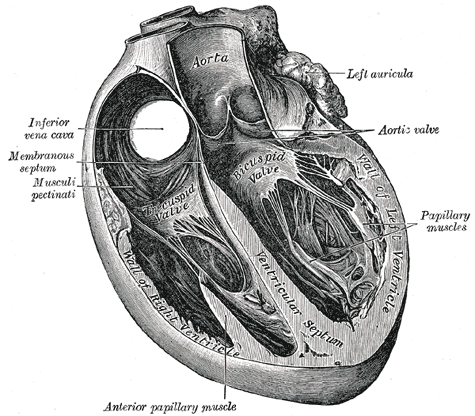
\includegraphics[width=0.7\textwidth]{figures/sample/Gray498.png} 
\caption[Four-chamber illustration of the human heart.]{Four-chamber illustration of the human heart.  Clockwise from upper-left: right atrium, left atrium, left ventricle, right ventricle.}
\label{fig:fourchamber}\end{figure}

The use of acoustic waves for medical diagnosis, inspired by naval sonar, was initially developed in the 1940s \cite{gagliardi_ultrasonography_1996}.  By 1954, the first clinically useful cardiac ultrasound -- examining motion of the mitral valve in stenosis -- was reported \cite{edler_ultrasonic_1957}.  These early scans were one-dimensional images (`A-mode'), sometimes repeated to generate a time axis (`M-mode').   The sector-scanning probe was developed in the 1970s \cite{bom_ultrasonic_1971,griffith_sector_1974}, leading to the `B-mode' that a modern cardiologist would recognise as an echocardiogram.

\chapter{Introduction}
\label{ch:intro}

%\section{Background}
%\label{s:background}

The notion of describing amorphous materials as random networks dates back to \zach, who in 1932 sketched a simple diagram of a \td{} glass \cite{Zachariasen1932}.
This configuration, reproduced in figure \ref{fig:zach_orig}, showed a collection of percolating rings with an absence of long\--range structural ordering.
At the time, \zach's image was intended only as schematic to illustrate the analogous effects in \thd{} glasses.
However, some eighty years later, modern synthesis techniques have yielded a range of \td{} materials including amorphous carbon, silica and germania, which can be considered realisations of \zach's glass \cite{Kotakoski2011,Robertson2012,Huang2012,Lichtenstein2012a,Shaikhutdinov2013,Lewandowski2018,Lewandowski2019}.
These advances may yet represent a watershed moment in chemistry, facilitating the development of a wide range of technologically useful materials with applications including catalysis and gas separation \cite{Trogadas2014,Sun2015a,Buchner2017}.

It is clear that understanding the structure of amorphous materials is key to this aim.
However, due to the relative recentness of these experimental discoveries, much of the existing theory arises from studies of systems on greater length scales.
Specifically, in the second half of the 20\th{} century, much work was carried out on the formation of polycrystals in metals and alloys.
By annealing the metal and slicing through the sample, the grains in the polycrystal could be directly imaged; revealing a system of tessellating polygons not dissimilar to an atomic material \cite{Beck1954,Dunn1957}.

Over time it became apparent that the structure of these networks is constrained on a number of different levels.
Firstly the mean ring size (\ie{} the average number of sides in a polygon) tends to the constant value of six.
This is readily explainable via graph theoretic arguments, resulting from Euler's formula when each vertex forms part of three edges - as is the case for trivalent atoms or the meeting of three grain boundaries.
This is consistent with chemical intuition: a pristine graphene sheet is a hexagonal net and although a Stone\--Wales defect introduces pentagons and heptagons, they occur in pairs to preserve the overall mean ring size \cite{Stone1986}.

The next level of information is then the explicit distribution of polygon sizes, also known as the ring statistics.
With the constraint of a fixed mean, the ring statistics were shown to be relatively well defined, following a lognormal or maximum entropy distribution \cite{Shackelford1981,Lemaitre1993,Lichtenstein2012}.
However, the ring statistics alone are not sufficient to fully describe the network topology. 
This is because the same set of rings can be arranged in a large number of different ways.
Consider again \zach's original configuration. 
Removing one square achieves a mean ring size of six and allows the constituent rings to be arranged as a periodic tiling.
Figures \ref{fig:zach_high}\--\ref{fig:zach_low} show three such example tilings.


\begin{figure}[h]
     \centering
     
     \begin{subfigure}[b]{0.25\textwidth}
         \centering
         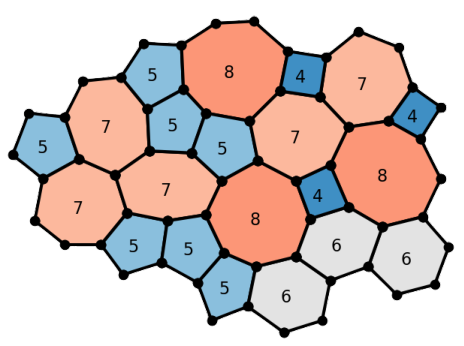
\includegraphics[width=\textwidth]{./figures/introduction/zach_orig.pdf}
         \caption{}
         \label{fig:zach_orig}
     \end{subfigure}
     \hspace{1cm}
     \begin{subfigure}[b]{0.25\textwidth}
         \centering
         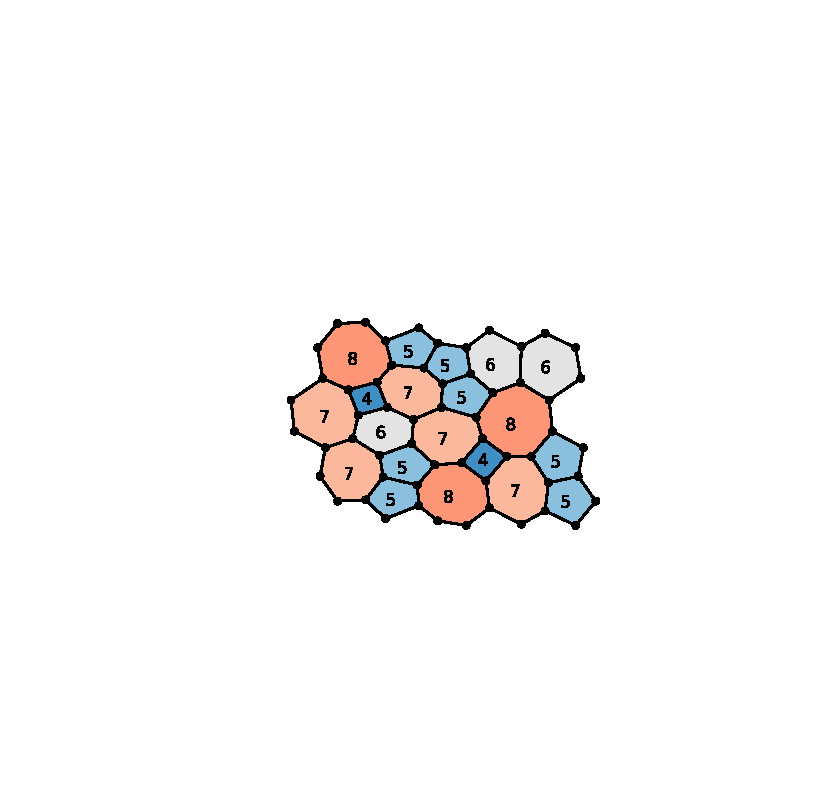
\includegraphics[width=\textwidth]{./figures/introduction/zach_high.pdf}
         \caption{}
         \label{fig:zach_high}
     \end{subfigure}
     
     \begin{subfigure}[b]{0.25\textwidth}
         \centering
         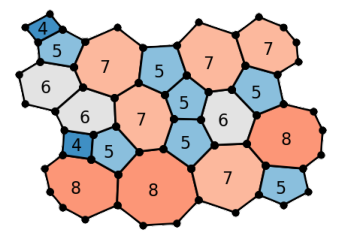
\includegraphics[width=\textwidth]{./figures/introduction/zach_mid.pdf}
         \caption{}
     \end{subfigure}
     \hspace{1cm}
     \begin{subfigure}[b]{0.25\textwidth}
         \centering
         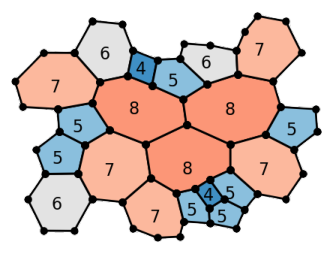
\includegraphics[width=\textwidth]{./figures/introduction/zach_low.pdf}
         \caption{}
         \label{fig:zach_low}
     \end{subfigure}
     
     \caption{Panel (a) shows \zach's glass and panels (b)\--(d) three different periodic arrangements based on the glass (with one square removed to satisfy Euler's formula). Moving from panel (b)\--(d) there is increased clustering of similar sized rings. The size of the rings are highlighted numerically and by colour.}
     \label{fig:zach}
\end{figure}

Whilst they may initially look similar, on closer inspection the three configurations display fundamentally different properties.
In figure \ref{fig:zach_high} similar sized rings are dispersed throughout the arrangement whilst in \ref{fig:zach_low} they are tightly clustered together.
Furthermore, given the large number of configurations which may be theoretically possible for any set of ring statistics, only a subset of these are physically realisable.
Empirically, these are found to be those in which large rings tend to be surrounded by smaller rings \ie{} similar to \ref{fig:zach_high}.
Once again, chemical intuition would support this in the context of atomic materials, as strain is minimised by maintaining bond lengths and angles as close to their equilibrium values as possible.

This effect was first noticed in polycrystals and quantified through the \aw{} law \cite{Aboav1970,Weaire1974}.
This law posits that the mean ring size about any given ring can be related to the central ring size by a single fitting parameter.
Hence the value of this parameter in some way describes the increased tendency of the small rings to be adjacent to large rings.
The \aw{} parameter therefore provides information on the first\--order ring\--ring correlations, completing the topological description of the network material.

The novelty and potential usefulness of \td{} materials makes them a  clear candidate for computational study, in order to complement and supplement experimental endeavours. 
Taking the example of thin silica films, there have already been multiple computational investigations including both \abinitio{} methods and molecular dynamics studies using classical force fields at varying levels of theory \cite{Bjorkman2013,Malashevich2016,Wilson2013,Wilson2018,Zhang2018a,Bamer2019,Roy2019,Richter2019}.
In order to perform these simulations, it is necessary to have a starting atomistic configuration.
This can be achieved in multiple ways. 
The most straightforward is to take one of the existing experimental images. 
These are however limited in size and number and can contain defects or areas which cannot be fully imaged.
In addition, some related experimental systems have proved significantly more challenging to synthesise, such as bilayers of germania, restricting the experimentally available data  \cite{Lewandowski2018,Lewandowski2019}.
As a result, computational techniques are often preferable, but generating configurations will the required topological properties (\ie{} correct ring statistics \textit{and} \aw{} parameter) has proved surprisingly difficult \cite{Roy2018,Kumar2014}.

Therefore, the first part of this thesis will focus on developing methods to generate configurations of \td{} networks in which the topological parameters can be tuned in a controllable manner.
These configurations can then be used as a seed for further computational studies, removing some of the reliance on experimental configurations and opening the door for high\--throughput calculations which can be speculative and potentially predictive.

However, the scope of this work extends beyond materials modelling.
As previously mentioned, much of the original work in this field focussed on polycrystals of metal oxides, with some links to foams and Voronoi polygons \cite{Aboav1980,Boots1984}.
It is now clear that these chemical networks fit into a much wider class of \td{} physical networks that are ubiquitous in the natural world, emerging across physical disciplines and length scales.
Traditional examples range from the atomic level of ultra\--thin materials, through colloids, foams, epithelial cells and all the way to geological rock formations \cite{Earnshaw1994,Allain1995,Moncho-Jorda2000,Durand2011,Tong2017,Goehring2014}.
There are however countless more occurrences, with drying blood, stratocumulus clouds, crocodile scales and geopolitical borders all being the subject of studies \cite{Brutin2011,Glassmeier2017,Milinkovitch2019,LeCaer1993}.

Intriguingly, although these systems are incredibly physically diverse, they have strikingly similar structures \cite{Schliecker1999}. 
This is because they can all be mapped onto the same generic system, which can be equivalently described as a collection of tessellating polygons or percolating rings, and hence they are governed by the same fundamental laws. 
Understanding the behaviours of \td{} networks is therefore key to a wide range of problems in frontier research, not only the directed synthesis of nano\--materials but also for example the control of mitotic division \cite{Gibson2011,Ladan2019}; as well as to curiosities such as explaining the arrangement of the stones in Giant's Causeway or cracking in famous artworks \cite{Weaire1984,Flores2017}.

Coupled with these observations, the continuing expansion and maturity of network science as a field has led to significant advances in the description and characterisation of complex networks.
This has largely been driven by interest in networks in the more abstract sense of the internet, social media and neural networks \cite{Strogatz2001,Boccaletti2006,Barabasi2012}.
To date, the application of these principles in the physical sciences has mostly been confined to topics such as biological signalling pathways.
However, network science is also highly relevant to the study of atomic systems, where the notions of collections of bonded atoms map straightforwardly onto the definition of complex networks as a set of linked nodes.

The second part of this thesis will therefore show how robust metrics from network science can be applied to physical \td{} networks to better quantify their structure and replace the need for empirical measures such as the \aw{} law.
As part of this process, more generic methods will be developed to construct \td{} networks across a range of potential models, coordination environments and topologies.
This will allow a systematic study into the factors which influence the underlying network properties in \td{} systems.
More broadly, this will have the effect of tying physical \td{} networks into the wider field of network science, showing them to be a unique and interesting addition to the area.

The later parts of this thesis will apply the developed concepts and techniques to a series of related and novel problems across chemistry.
To give a broad overview, this will begin with an investigation into the network analysis of quasi\--two\--dimensional hard sphere systems, which is of direct relevance to on\--going experimental studies of colloidal monolayers \cite{Thorneywork2017}.
In such systems, the ring structure emerges through construction of a Voronoi diagram, which partitions the sample space into polygonal regions associated with each particle.
Whilst the properties of Voronoi diagrams are well understood for two\-- and three\--dimensional systems, the intermediate dimensionality of colloidal monolayers leads to novel challenges in their characterisation.

Following this, attention will be turned to another system of relatively recent interest, that of ``procrystalline'' lattices \cite{Overy2016}.
These procrystals can also be considered to have intermediary behaviour, in that they have atoms located on a regular, ordered lattice and yet have disordered ring structure - hence lying between the crystalline and amorphous states.
This partial ordering raises the possibility of procrystals displaying fundamentally different behaviour, in terms of their network properties, to either crystalline or amorphous materials.

Finally, a new tool from topological data analysis, termed persistent homology, will be applied to \td{} amorphous materials.
The aim of persistent homology is to find the fundamental topological features in generic point sets, and so holds the potential to identify and characterise the ring structure in atomic networks \cite{Wasserman2018}.
Although the method is in its relative infancy, the effectiveness of persistent homology in quantifying disorder in the case of \td{} materials can be examined ahead of time through the use of computational models.

These interrelated examples raise two important questions central to this work, namely why is the focus on \td{} systems, and why on computational modelling?
To answer the first of these questions, one may argue it is precisely because there exist experimental realisations of quasi\--two\--dimensional systems, which have a range of technologically useful applications \cite{Butler2013,Bhimanapati2015,Tan2017}.
Alternatively, it may be said that a \td{} system is in some way a simplified version of a \thd{} assembly, and so they provide a tractable way of studying the behaviours of higher dimensionality systems.
Whilst both these statements have merit, neither is entirely satisfactory, as the former neglects to explain why such experiments are successful and latter is not universally true \cite{ChaikinPaulM1995}.
Two\--dimensional systems can display their own unique constraints, which in fact often leads to the desirable properties of nanomaterials.

What study in two dimensions provides, is the opportunity to visualise, analyse and understand systems which are inherently more tangible.
Raw data is available experimentally in real\--space, without the need for transformation, as required for example with structure factors or diffraction patterns.
From this data, metrics such as the ring structure are well defined and readily extractable.
This in turn allows the development of simulation and analysis methods which are able to accurately model and characterise the system, leading to a more complete understanding.
Ideally, the insight gained can be applied to higher dimensions, or used to aid the synthesis of materials with desired properties.

In response to the second question, the power of computational modelling as complement to experiment arises from the ability to reproduce experimental results, but also explore experimentally inaccessible systems.
As previously mentioned, experimental microscopy data from frontier research is difficult to produce and may be incomplete or relatively small in extent.
Computational models can help to bridge any gaps and provide information as to the frequency or stability of the observed sample.
Moreover, computation has direct access to a greater number of observables than experiment, which can help provide explanation for a given phenomenon.
Finally, and perhaps most importantly, simulation allows a holistic study of materials by continuously varying parameters to generate structures which may or may not map onto those from experiment.
This enables properties to systematically explored, in principle leading to the holy grail of computational modelling, that of predictive capability.

This thesis will incorporate many of the above aspects to investigate the phenomenon of structural disorder in \td{} network\--forming materials.
Computational models and methods will be developed to simulate a wide range of \td{} systems.
This will be achieved almost exclusively through the use of stochastic \mc{} algorithms.
These tools will be designed with flexibility in mind, aiming to generate configurations in which the ring topologies can be precisely controlled.
In most cases, whilst the underlying models will remain physically motivated, the specificities of the system will be abstracted into a more generic network problem.
This will allow comparisons to be made between initially seemingly disparate materials and enable development of a generalised network theory for physical \td{} systems.

Nevertheless, the motivation for this work is still ultimately grounded in the characterisation and development of real materials.
Contact will therefore be made to experimental results and the applicability and relevance to experimental investigations will be detailed throughout.
In particular, this thesis will aim to improve the modelling of amorphous bilayers, evaluate analysis methods for thin\--films and colloidal packings, and direct the synthesis of procrystalline materials.  

%\section{Thesis Structure}
%
%The structure of this thesis is as follows:
%\davidnote{Todo: thesis structure}
%\davidnote{Just basically a repeat of abstracts?}
%\davidnote{Actually can this section just go?}
%
%\begin{itemize}
%	\item \textbf{Chapter 2}: the theory underpinning complex networks is discussed, covering the representation of atomic systems as networks and the relationship of the dual network to ring structure.
%The laws which govern the topological properties of physical networks are also introduced, namely Euler's law, \lm's law and the \aw{} law.
%
%	\item \textbf{Chapter 3}: the theoretical basis of \mc{} methods and their application to generating realisations of \td{} networks is reviewed.
%There is a broad discussion of Metropolis \mc{} methods, before specific methods are covered in detail; namely the bond switching algorithm and hard particle \mc{} in conjunction with the Voronoi construction.
%This discussion lays the groundwork for the extension of these methods and development of additional \mc{} algorithms in subsequent chapters.
%	
%	\item \textbf{Chapter 4}: a computationally tractable \mc{} method using triangle rafts is developed to generate bilayers of \sioii{} and related materials.
%The method allows defect free networks of any given shape to be grown with both tuneable ring statistics and topologies, controlled by a combination of the choice of the ``allowed'' rings and the effective growth ``temperature''. 
%Configurations are generated with \aw{} parameters commensurate with those obtained from an analysis of experimental configurations, improving significantly on previous methods.
%The ability to efficiently grow configurations allows exploration of the structural basis of \lm’s law, where the commonly observed value of $p_6\approx0.4$ is presented as a balance between entropic and enthalpic factors. 
%The deviations of ring areas from the ideal values are discussed and the relative insensitivity of the ring area to relatively strong distortions is highlighted.
%	
%	\item \textbf{Chapter 5}:
%	
%	\item \textbf{Chapter 6}:
%	
%	\item \textbf{Chapter 7}:
%	
%	\item \textbf{Chapter 8}:
%
%	\item \textbf{Chapter 9}:
%	
%	\item \textbf{Chapter 10}:
%\end{itemize}
	
 

\chapter{Network Theory}
\label{ch:networktheory}

\begin{chapterabstract}
The theory underpinning complex networks is discussed, covering the representation of atomic systems as networks and the relationship of the dual network to ring structure.
The laws which govern the topological properties of physical networks, namely Euler's law, \lm's law and the \aw{} law are also introduced.
\end{chapterabstract}

\section{Network Theory}
\label{sec:networktheory}

The scope of what constitutes a complex network is extremely broad, covering everything from the tangible (\eg{} computational clusters) to the more abstract (\eg{} social interactions). Yet part of the appeal and power of network science is the ability to quantify and relate these highly disparate systems with the same underlying theory.
A network is simply a collection of components termed \textit{nodes} and the connections between them termed \textit{links}, an example of which is given in figure \ref{fig:smallnet}.
There are then two fundamental classes of network based on the nature of the connections.
Networks in which the links between nodes are mutual are termed undirected, whereas those in which the links are one\--way are termed directed \cite{barabasi2016n}.
At the risk of dating this thesis, this is the difference between Facebook (an undirected social network of friends) and Twitter (a directed social network of followers).
All the networks considered in this work are undirected and all the theory assumes this property.

\begin{figure}[ht]
     \centering
      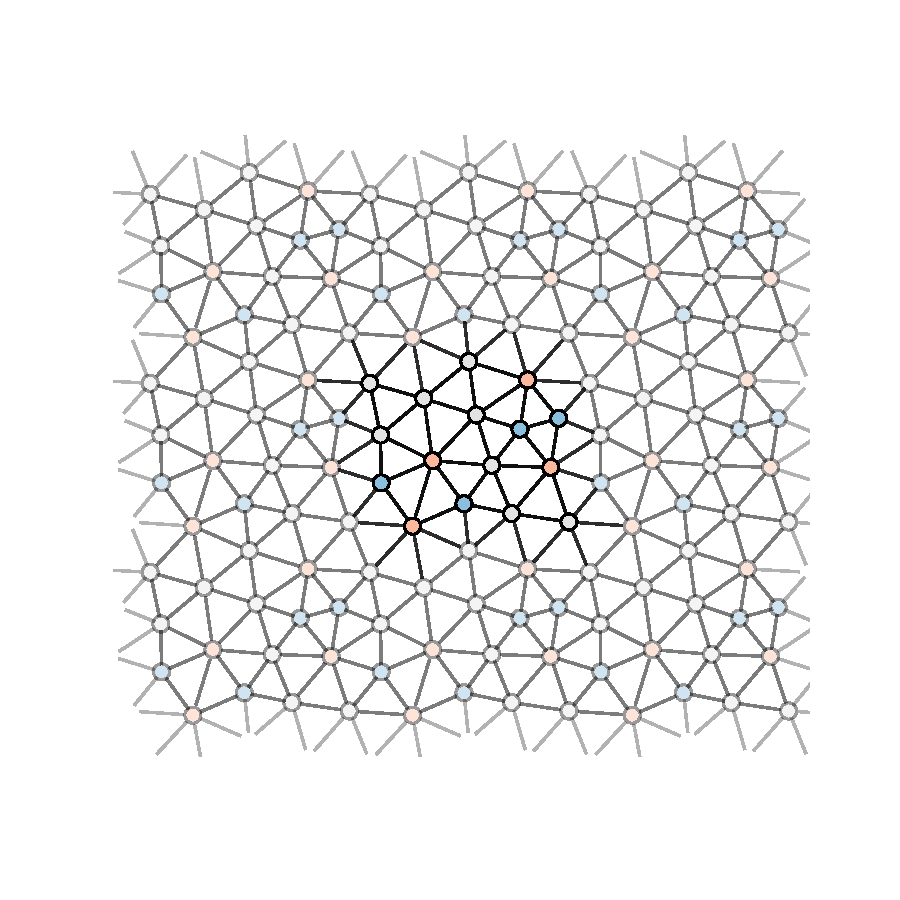
\includegraphics[width=8cm]{./figures/methods/small_periodic_net.pdf}
     \caption{Example of a periodic \td{} network where nodes are represented by circles and links as lines. Nodes are coloured similarly according to their degree, whilst periodic images are greyed out to highlight the central repeating unit.}
     \label{fig:smallnet}
\end{figure}

\subsection{Node Degree and Probability Distributions} 

A key concept in network science is the the node degree, defined as the number of links that each node possesses.
A node with $k$ links is then said simply to have degree $k$, where $k\in\mathbb{N}$.
This is illustrated in figure \ref{fig:smallnet}, which consists of 5\-- (blue), 6\-- (grey) and 7\-- (red) degree nodes.
The occurrence and correlations of nodes of given degrees can then be described by a range of probability distributions.

The probability of a randomly selected node having degree $k$ is given by the node degree distribution, denoted $p_k$.
This is a normalised discrete distribution such that
\begin{equation}
	\label{eq:pknorm}
	\sumk p_k = 1 \,.
\end{equation}
The $n$\th{} moments of this distribution are then given by:
\begin{equation}
	\label{eq:pkmoment}
	\langle k^{n} \rangle = \sumk k^np_k \,.
\end{equation}
Alternatively, one can also calculate the probability that a randomly selected link has a $k$\--degree node at the end, denoted $q_k$.
This is not the same as the distribution above, as there is greater chance of selecting links which emanate from high degree nodes, in a manner which is proportional to the node degree.
As this distribution is normalised, this leads to the relations:
\begin{align}
	\sumk q_k &= 1 \label{eq:qknorm} \\
	q_k &= \frac{kp_k}{\langle k \rangle} \label{eq:qkpk} \,.
\end{align}
In addition, one can also evaluate the probability that a randomly chosen link has nodes of degree $j$,$k$ at either end.
This is the node joint degree distribution, denoted $e_{jk}$. 
Once again this is normalised and satisfies the following relationships:
\begin{align}
	\sumjk e_{jk} &= 1, \label{eq:ejknorm} \\
	\sumjk e_{jk} &= q_j \label{eq:ejkqk} \\
	e_{jk} &= e_{kj} \label{eq:ejkekj} \,,
\end{align}
where the final result arises from reciprocal nature of the links in an undirected network.
As an example, these three probability distributions are provided for the network in figure \ref{fig:smallnet}:
\begin{align}
	\mathbf{p} =  \frac{1}{16} \, \begin{blockarray}{*{1}{c} l}
	\begin{block}{[*{1}{c}]>{$\footnotesize}l<{$}}
	4 \: \bigstrut[t]& 5\\
	8 & 6 \\
	4 & 7 \\
	\end{block}
	\end{blockarray}
	\qquad
	\mathbf{q} =  \frac{1}{96} \, \begin{blockarray}{*{1}{c} l}
	\begin{block}{[*{1}{c}]>{$\footnotesize}l<{$}}
	20 \: \bigstrut[t]& 5\\
	48 & 6 \\
	28 & 7 \\
	\end{block}
	\end{blockarray}
	\qquad	
	\mathbf{e} = \frac{1}{96}\: \begin{blockarray}{*{3}{c} l}
	\begin{block}{*{3}{>{$\footnotesize}c<{$}} l}
	5 & 6 & 7 \\
	\end{block}
	\begin{block}{[*{3}{c}]>{$\footnotesize}l<{$}}
	2 & 9 & 9 \: \bigstrut[t]& 5\\
	9 & 22 & 17 & 6 \\
	9 & 17 & 2 & 7\\
	\end{block}
	\end{blockarray} \, .
%	\textbf{p} = \frac{1}{96}\: \begin{blockarray}{*{5}{c} l}
%	\begin{block}{*{5}{>{$\footnotesize}c<{$}} l}
%	3 & 6 & 7 & 8 & 9 \\
%	\end{block}
%	\begin{block}{[*{5}{c}]>{$\footnotesize}l<{$}}
%	0 & 0 & 5 & 10 & 1\: \bigstrut[t]& \:3\\
%	0 & 0 & 1 & 1 & 0 & \:6 \\
%	5 & 1 & 14 & 14 & 1 & \:7\\
%	10 & 1 & 14 & 14 & 1 & \:8\\
%	1 & 0 & 1 & 1 & 0 & \:9\\
%	\end{block}
%	\end{blockarray}
\end{align}

\subsection{Atomic and Ring Networks}
\label{s:atomringnetworks}

To see how network theory relates to atomic materials, consider the amorphous graphene configuration in figure \ref{fig:graphdualgraph}.
In this network the nodes represent carbon atoms and the links sp$^2$ bonds.
The node degree in the atomic network for all nodes is then equal to three, being equivalent to the atomic coordination number (which throughout this thesis will be denoted by $c$).
This is problematic, because whilst there is clear disorder in the system, it is not well captured by the atomic network.
Due to the fact that the local environment around the atoms is identical, when examining say the node degree distribution any information about the glassy structure is lost.
This network is to first order indeterminable from a crystalline hexagonal lattice.

\begin{figure}[bt]
     \centering
     
     \begin{subfigure}[b]{0.3\textwidth}
         \centering
         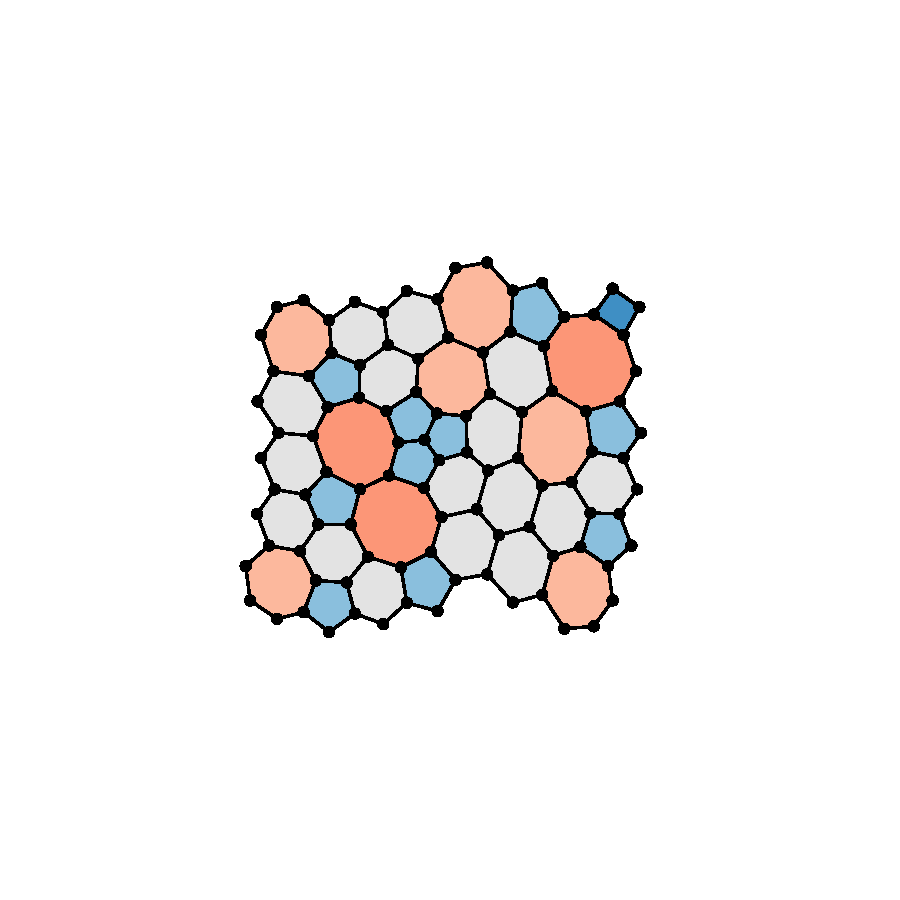
\includegraphics[width=\textwidth]{./figures/methods/graph.pdf}
         \caption{Atomic network.}
         \label{fig:graphdualgraph}
     \end{subfigure}
     \hfill
	\begin{subfigure}[b]{0.3\textwidth}
         \centering
         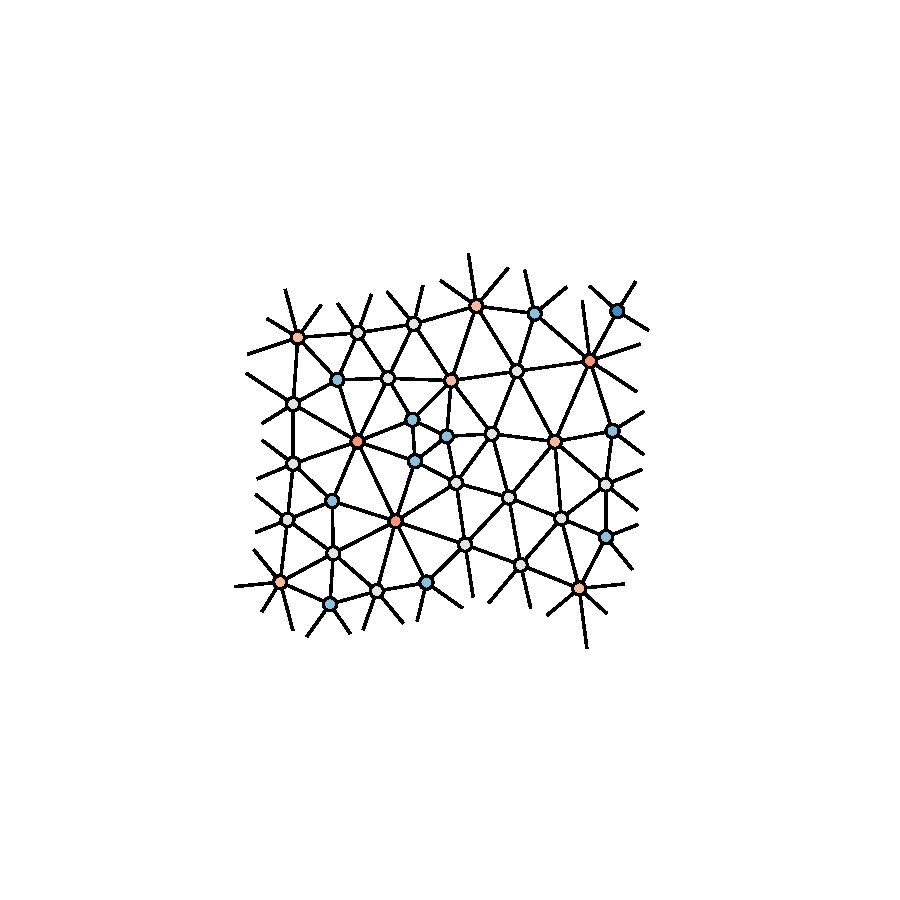
\includegraphics[width=\textwidth]{./figures/methods/dual.pdf}
         \caption{Ring network.}
         \label{fig:graphdualdual}
     \end{subfigure}
     \hfill
     \begin{subfigure}[b]{0.3\textwidth}
         \centering
         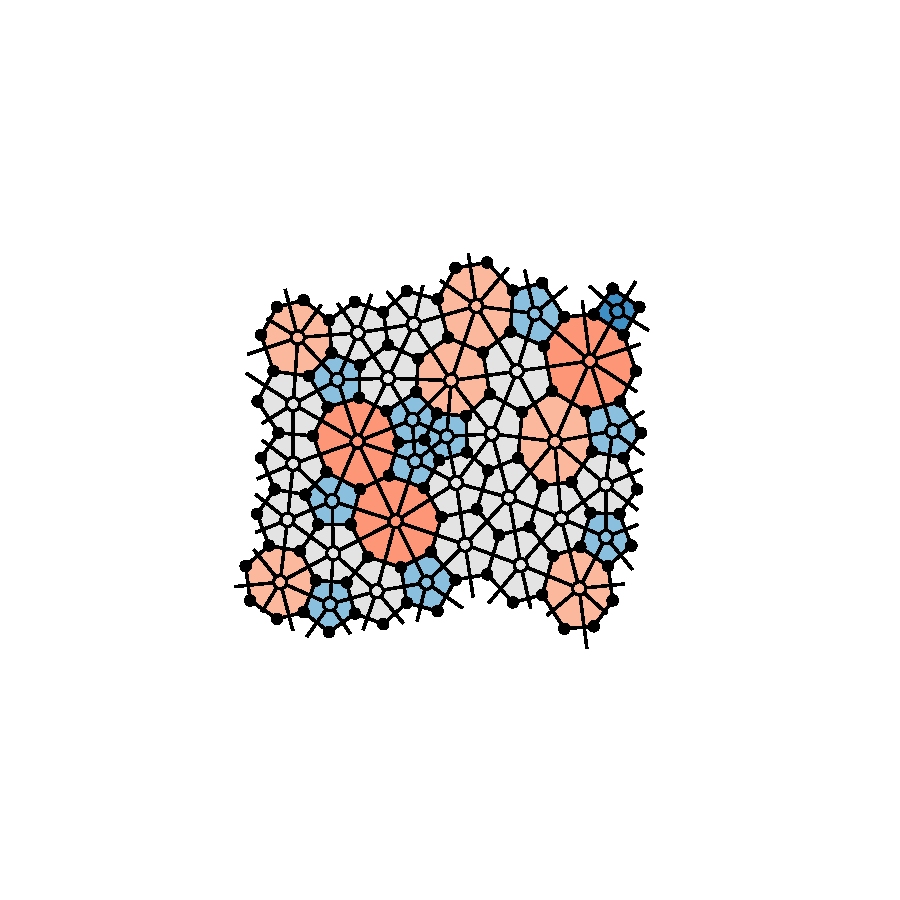
\includegraphics[width=\textwidth]{./figures/methods/graph_dual.pdf}
         \caption{Dual relationship.}
         \label{}
     \end{subfigure}
     \hfill
     
     \caption{Panel (a) gives an example of a 3\-- coordinate periodic atomic network with disordered ring structure. Nodes and links represent atoms and bonds respectively where rings are coloured by size. Panel (b) gives the corresponding ring network where nodes and links represent rings and their adjacencies, where nodes are coloured by degree. Panel (c) shows the dual relationship between the atomic and ring networks, where the node degree in the ring network is equal to the ring size in the atomic network.}
     \label{fig:graphdual}
\end{figure}

Observing figure \ref{fig:graphdualgraph} one can see there is another level of structure in the network, namely that of the ring structure.
A ring is strictly any closed path of sequentially linked nodes in a network, but this thesis will use the term in reference only to the primitive rings \ie{} those which cannot be subdivided into two smaller rings \cite{Yuan2002}.
A ring of size $k$ (or $k$\--ring) is then defined as a ring with $k$ constituent nodes.
It is clear that finding and counting the number of rings of each size, often termed calculating the ring statistics, does then quantify the disorder in the system \cite{Kumar2014}.
The ring statistics can be summarised by the normalised probability distribution, $p_k$.

However, there is a more efficient way of representing and quantifying the ring structure in the system, and that is by constructing the dual network \cite{Aboav1984}.
The dual is generated by placing a node at the centre of each ring and linking the nodes of adjacent (\ie{} edge\--sharing) rings, as can be seen in figure \ref{fig:graphdualdual}.
This will be referred to as the ring network.
The ring network is a reciprocal lattice in which the node degree, $k$, is equivalent to the ring size in the atomic network.
Similarly, it consists solely of triangles, reflecting the 3\--coordinate nature of the underlying atomic network.
Hence, the disorder is captured directly in the node properties of the ring network.
These characteristics make the ring network preferable for manipulating and analysing the systems in this thesis.

\section{Topological Laws}
\label{s:topolaws}

There are a number of laws which govern the topological properties of \td{} network\--forming materials.
These laws constrain the ring structure, influencing the network properties in a manner that makes physical networks unique in the field of network science.
These laws act on a number of ``levels'': Euler's law controls the overall mean ring size, \lm's{} law the ring size distribution and the \aw{} law the ring\--ring correlations.

\subsection{Euler's Law}
\label{s:eulerslaw}

Euler's law constrains the mean ring size, $\ki$, in an atomic network or equivalently the mean node degree of the ring network.
The atomic networks studied in this work are all \td{}, connected (there is a path between any two nodes) and planar (they have no overlapping links) and so are subject to Euler's formula which states:
\begin{equation}
	\label{eq:eulerformula}
	N + V - E = \chi,
\end{equation}
where $N$, $V$, $E$ are the number of rings, vertices and edges in the network and $\chi$ in an integer termed the Euler characteristic, which is dependent on the global topology of the system.
Each vertex represents an atom and the number of edges emanating from each vertex is then the coordination number.

For generality consider an atomic network with atoms of assorted coordination numbers, $c$. 
If the proportion of each coordination type is $x_c$, then the mean coordination number is given by $\langle c \rangle = \sum\limits_c cx_c$.
This allows the number of edges to be written in terms of the number of vertices as $E=\frac{V}{2}\langle c \rangle$. 
In turn the mean ring size is simply the total number of vertices per ring, allowing for multiple counting, such that $\ki=\frac{V}{N}\langle c \rangle$.
Substituting these two expressions into equation \eqref{eq:eulerformula} leads to the expression:
\begin{equation}
	\label{eq:avdegree}
	\ki = \frac{2\langle c \rangle\left(1-\chi/N\right)}{\langle c \rangle - 2}.
\end{equation}
Hence the average node degree in the ring network (equivalent to the mean ring size of the physical network), is simply related to the average degree of the physical network (\ie{} local coordination environment), the topology of the system and the number of rings.

Although equation \eqref{eq:avdegree} may appear simple, it is a very powerful constraint. 
To demonstrate this consider a two\--dimensional lattice with two possible coordination environments $c=3,4$. 
The planar case with periodic boundary conditions (mimicking an infinite planar lattice) maps onto the torus with $\chi=0$, and so:
\begin{equation}
	\label{eq:2dplanarcases}
	\ki = \begin{cases}
		6, \quad x_3 = 1 \\
		4, \quad x_4 = 1 \\
		5, \quad x_3 = 2/3, x_4 =1/3
	\end{cases}\,.
\end{equation}
To reiterate in plain terms, this means that if there is a material consisting of atoms all forming exactly three bonds (as for amorphous carbon), the mean ring size \textit{must} be equal to six. 
Similarly if all atoms form four bonds the mean ring size is four, and if there is a two\--thirds to one\--third mixture of coordination environments the mean ring size is five.
The simplest illustrations of these are the hexagonal, square and cairo regular tilings, shown in figure \ref{fig:lattices}, but this law holds equally well for amorphous configurations.
For aperiodic systems strictly $\chi=1$, but as $N\rightarrow \infty$, the proportion of vertices with unsatisfied coordination on the sample perimeter become negligible overall as does the term in $\chi$.
Therefore in reality these relationships hold, and remain as applicable to amorphous graphene as the basalt columns in Fingal's Cave, and the Penrose tiling \cite{Goehring2014,Ressouche2009}.

This analysis also extends to spherical topology where $\chi=2$, and so:
 \begin{equation}
 	\label{eq:2dsphericalcases}
	\ki = \begin{cases}
		\frac{6N-12}{N}, \quad x_3 = 1 \\
		\frac{4N-8}{N}, \quad x_4 = 1.
	\end{cases}
\end{equation}
These relationships are the origin of the 12 pentagon rule for 3-coordinate fullerenes (the ``football problem''), or equivalently an ``8 triangle rule'' in the 4-coordinate case, as this is the only way to satisfy these equations if the allowed ring sizes are limited to $k=5,6$ and $k=3,4$ respectively (as in figures \ref{fig:latticesfull92}, \ref{fig:latticesfull98}) \cite{Fowler1996}.
Much of the richness in the behaviour of \td{} physical networks stems from this fundamental constraint on the network average degree.

\begin{figure}[bt]
     \centering
     
     \begin{subfigure}[b]{0.3\textwidth}
         \centering
         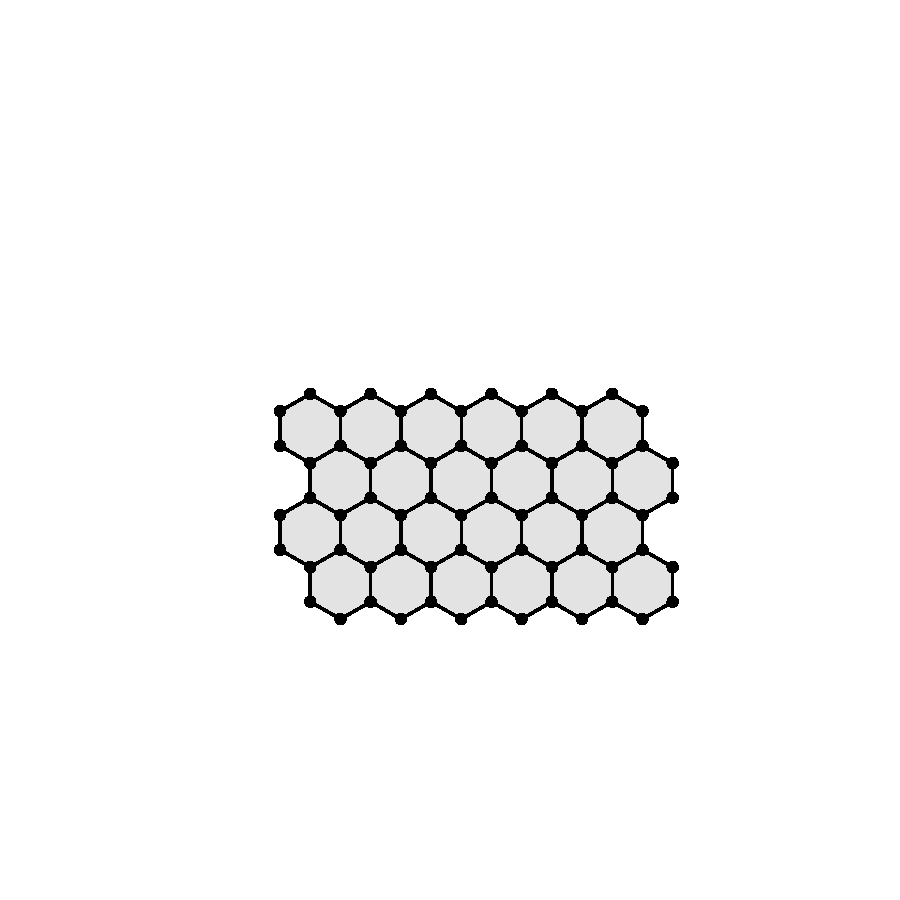
\includegraphics[height=2.4cm]{./figures/methods/hex.pdf}
         \caption{Hexagonal.}
         \label{fig:latticeshex}
     \end{subfigure}
     \hfill
     \begin{subfigure}[b]{0.3\textwidth}
         \centering
         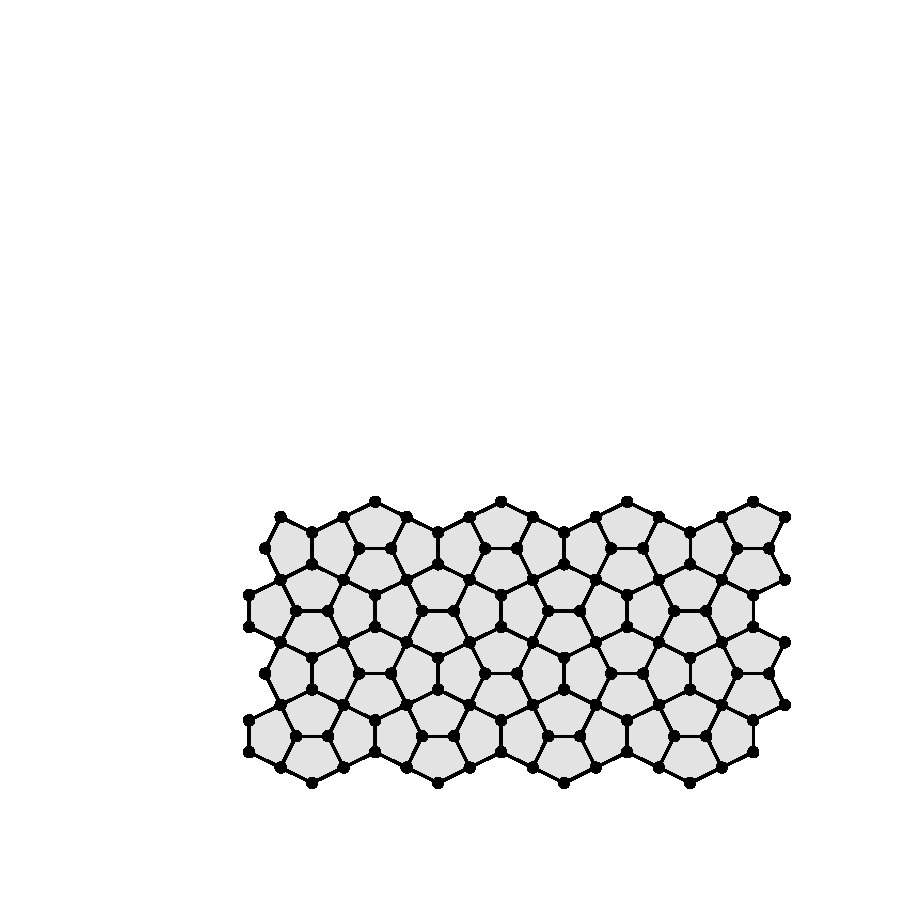
\includegraphics[height=2.4cm]{./figures/methods/cai.pdf}
         \caption{Cairo.}
         \label{fig:latticescairo}
     \end{subfigure}
     \hfill
	\begin{subfigure}[b]{0.3\textwidth}
         \centering
         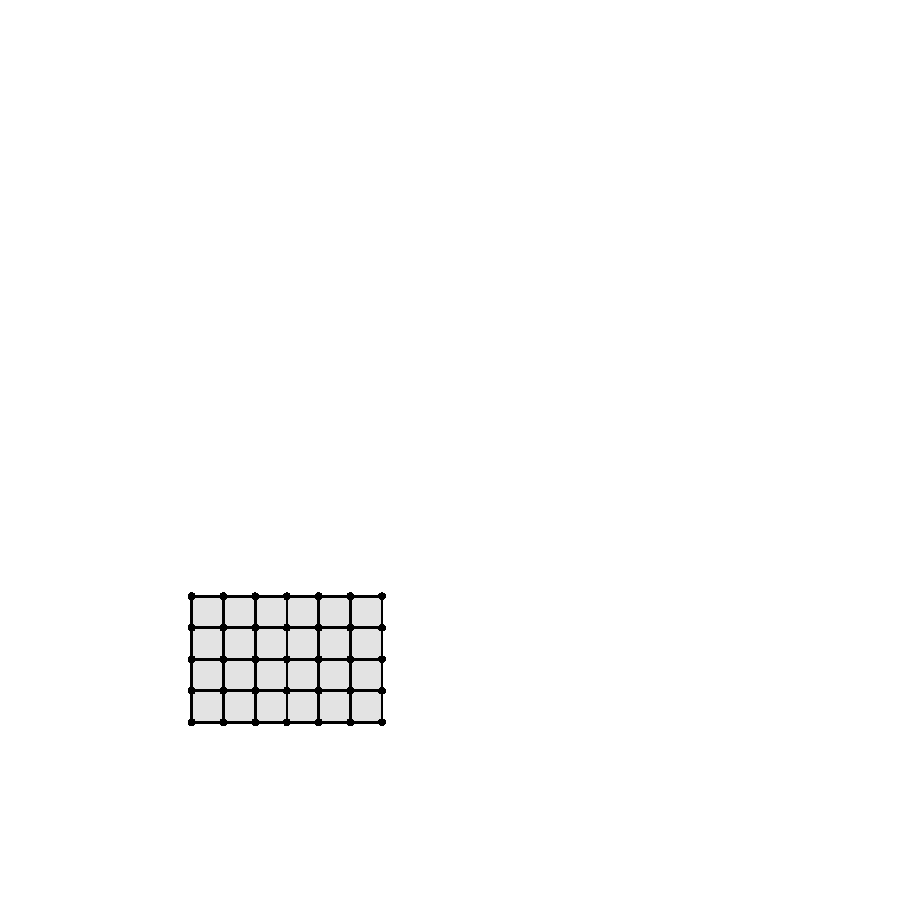
\includegraphics[height=2.4cm]{./figures/methods/sq.pdf}
         \caption{Square.}
         \label{fig:latticessq}
     \end{subfigure}
     \hfill
     \vspace{0.5cm}
     
       \begin{subfigure}[b]{0.45\textwidth}
         \centering
         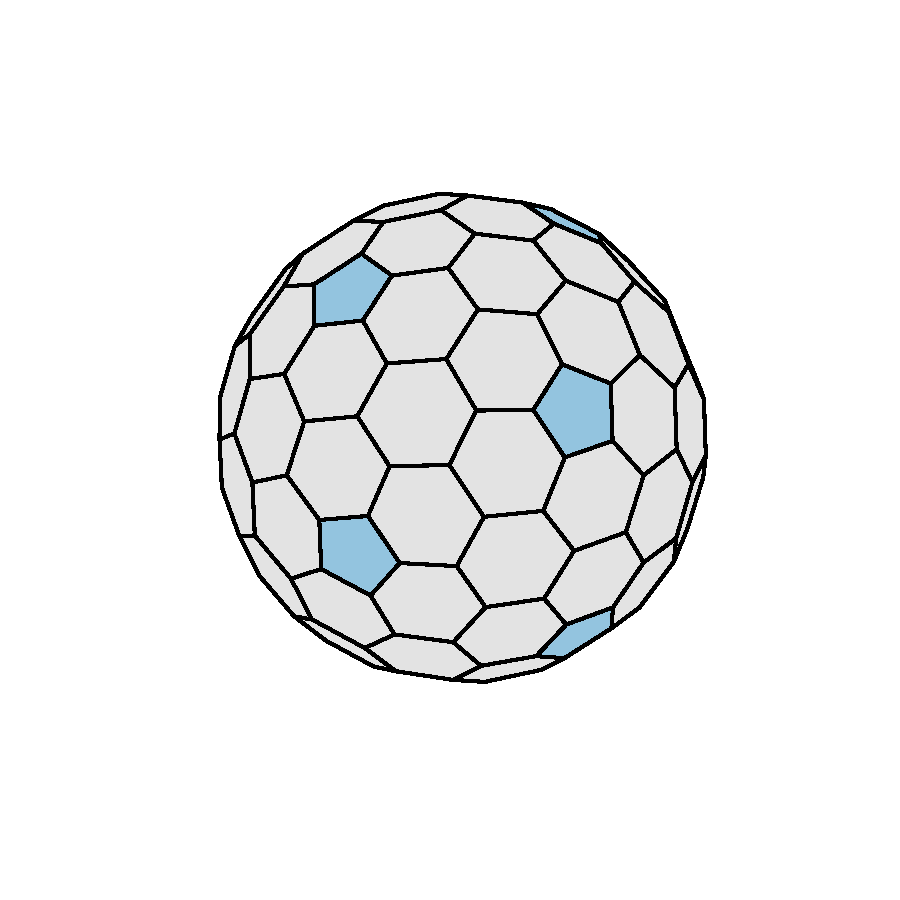
\includegraphics[height=2.4cm]{./figures/methods/full92.pdf}
         \caption{3\--coordinate fullerene.}
         \label{fig:latticesfull92}
     \end{subfigure}
     \hspace{1cm}
     \begin{subfigure}[b]{0.45\textwidth}
         \centering
         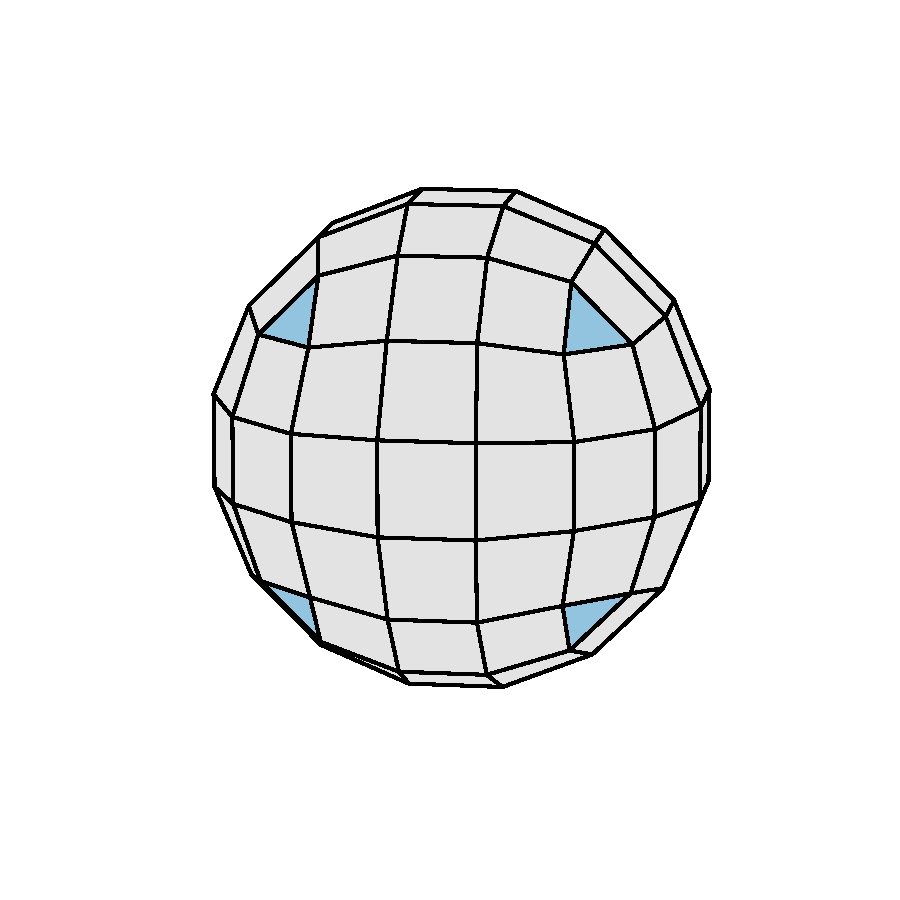
\includegraphics[height=2.4cm]{./figures/methods/full98.pdf}
         \caption{4\--coordinate fullerene.}
         \label{fig:latticesfull98}
     \end{subfigure}
     
     \caption{Panels (a)\--(c) give regular planar tilings of 6\--, 5\-- and 4\-- rings, where the ring size is related to the underlying atomic coordination. Panels (d) and (e) show the 3\-- and 4\-- coordinate tilings in spherical topology, where the mean ring size is reduced due to the change in the Euler characteristic.}
     \label{fig:lattices}
\end{figure}

\subsection{\lm's Law}
\label{s:lemaitre}

Knowing that the mean node degree is fixed by Euler's law, the next level of available information is the form of the underlying degree distribution, $p_k$.
Interestingly, the degree distributions found in physical ring networks seem relatively well defined.
For instance, it has been noted in models and realisations of \td{} silica glass that the ring statistics looked to follow a lognormal distribution \cite{Shackelford1981,Buchner2017}.
\lm{} \etal{} demonstrated that the distribution in 3-coordinate networks systems can be well described by a maximum entropy distribution \cite{Gervois1992}.
\lm's{} maximum entropy method is summarised here, trivially extended to arbitrary coordination.

The entropy of a probability distribution is defined as 
\begin{equation}
	\mathcal{S}=-\sumk p_k\log p_k. 
\end{equation}
In addition, the degree distribution has the following constraints:
\begin{align}
		\sumk p_k &=1, \\
		\sumk kp_k&=\ki,  \label{con:lm2}\\
		\sumk \frac{p_k}{k}&=\text{constant} \label{con:lm3},
\end{align}
where the first two constraints correspond to the normalisation condition and the fixed mean ring size, and the final constraint will be discussed below.
The entropy can then be maximised using Lagrange's method of undetermined multipliers to yield the result:
\begin{equation}
	\label{eq:mepk}
	p_k = \frac{e^{-\lambda_1 k - \lambda_2 / k}}{\sumk e^{-\lambda_1 k - \lambda_2 / k}},
\end{equation}
which can be solved numerically by substitution into equations \eqref{con:lm2},\eqref{con:lm3}. 
By allowing the chosen constant to vary, a family of maximum entropy curves can be generated, as in figure \ref{fig:lm1}.
The resulting distributions can be summarised by relating the variance, $\mu_2=\kii-\ki^2$, to a single chosen node degree probability, leading to the plot known as \lm's law, given in figure \ref{fig:lm2}.
It is usually framed in the context of the proportion of hexagons in a system, $p_6$, for the precise reason that most networks have $\ki=6$ and $p_6$ as the largest contribution.
Many experimental and theoretical studies have shown good agreement to this law \cite{Caer1993,Cerisier1996,Miklius2012}.

Simple extensions of the classic law are however possible, by modifying the mean degree or the permitted degree range.
For instance, $k$ is usually taken in the interval $k\geq3$ (as the triangle, $k=3$, is the smallest polygon), but there can be manifestations of physical systems where only certain degrees are accessible \cite{Rivier1988}.
Additional examples of such systems will be procrystalline lattices explored in chapter \ref{ch:procrystals}. 
The resulting \lm{} curves for a selection of these modifications are given in figure \ref{fig:lm3}. 
A discussion of these will be recur throughout this thesis, but one can see that the application of the allowable ring size constraints leads to marked differences in the maximum entropy solutions.
The maximum value of these curves can be simply determined by removing constraint \eqref{con:lm3}, equivalent to setting $\lambda_2=0$ in equation \eqref{eq:mepk}.
%Exploring these cases helps to understand the behaviour of \lm's law itself.
%By restricting the ring size to just $5\leq k \leq 7$ results in a straight line, which to satisfy Euler's law must have equation $\mu_2 = 1-p_6$.
%This line closely follows the high $p_6$ behaviour demonstrating that the initial deviation from the hexagonal lattice ($p_6=1$) is marked by the introduction of 5\-- and 7\-- ring defects.


\begin{figure}[bt]
     \centering
     
     \begin{subfigure}[b]{0.45\textwidth}
         \centering
         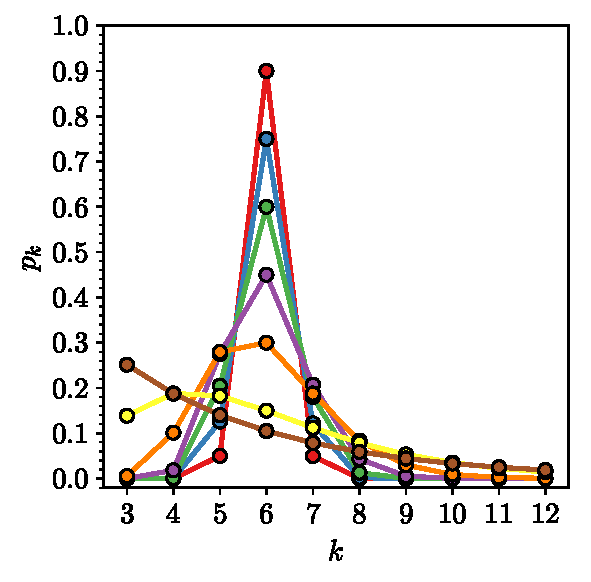
\includegraphics[width=\textwidth]{./figures/methods/lm_1.pdf}
         \caption{Maximum entropy distributions.}
         \label{fig:lm1}
     \end{subfigure}
     \hfill
      \begin{subfigure}[b]{0.45\textwidth}
         \centering
         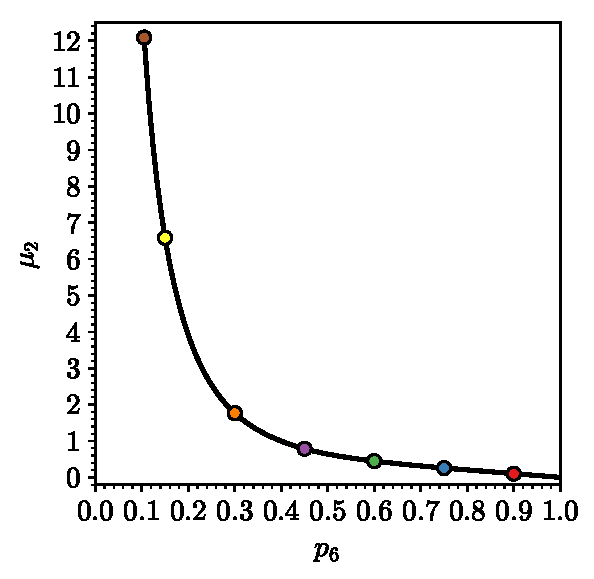
\includegraphics[width=\textwidth]{./figures/methods/lm_2.pdf}
         \caption{\lm's law.}
         \label{fig:lm2}
     \end{subfigure}
     \hfill
     
      \begin{subfigure}[b]{0.45\textwidth}
         \centering
         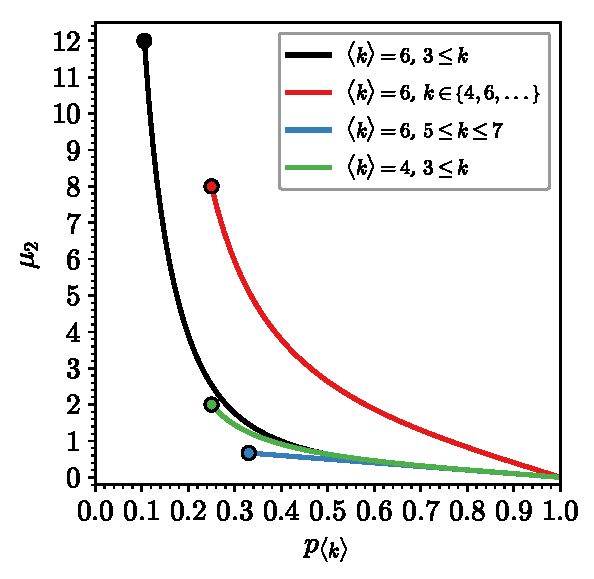
\includegraphics[width=\textwidth]{./figures/methods/lm_3.pdf}
         \caption{Extensions to \lm's law.}
         \label{fig:lm3}
     \end{subfigure}
     \hfill

    
     \caption{Illustration of \lm's maximum entropy method. Panel (a) gives examples of explicit maximum entropy distributions with different values of $p_6$. Panel (b) shows how these distributions can be summarised in a plot of $p_6$ \vs{} $\mu_2$ (\lm's law). Panel (c) provides extensions to the law by modifying the underlying constraints of the mean ring size and allowable $k$\--range.}
     \label{fig:lm}
\end{figure}

The only somewhat puzzling aspect of this successful theory is the choice of constraint \eqref{con:lm3}.
It was originally rationalised on the basis that the areas of rings of a given size, $A_k$, can be well fit by an expression $A_k = ak+b+c/k$, where $a$, $b$ and $c$ are constants.
As noted at the time, this is by no means true for all systems and in fact is contrary to the widely known Lewis law, which states that $A_k$ is linear in $k$ for many observable networks \cite{Lewis1928,Fortes1995,Kim2014}.
Despite this, the universality of the \lm{} law suggests that there must be a physical basis to \eqref{con:lm3}, and in the section \ref{s:assortativity} it will be demonstrated that it can be regenerated by considering ring adjacencies.

\subsection{\aw{} Law}
\label{s:awlaw}

The ring statistics given by \lm's law are an important measure for physical networks, but they do not provide a complete characterisation of the ring structure, as they say nothing about the ring adjacencies. 
This is important because whilst with the same ring statistics it is theoretically possible to organise the rings in many different arrangements, it is well known experimentally that only a subsection of these are observed.
The vast majority of physical systems have a preference for small rings ($k<\ki$) be adjacent to large rings ($k>\ki$).
This effect was first noted in the grains of polycrystals by Aboav \cite{Aboav1970}.
Aboav quantified these ring correlations by measuring the mean ring size about a $k$\--ring, denoted $m_k$, and found empirically that $m_k \approx 5 + 8/k$.

In an attempt to explain this observation, Weaire came across the following relation
\begin{equation}
	\label{eq:weairesumrule}
	\sumk km_kp_k = \sumk k^2p_k = \mu_2 + \ki^2 \,,
\end{equation}
known as Weaire's sum rule \cite{Weaire1974}.
From this he suggested the modification of $m_k=5+\left(6+\mu_2\right)/k$ which satisfied this rule.
Aboav's original equation then became a special case when $\mu_2=2$, which is close to the expected value for a random collection of Voronoi polygons (see section \ref{ssec:voronoi}).
Aboav then proposed that if a generic form of $m_k = A + B/k$ was used in conjunction with Weaire's sum rule then
\begin{equation}
	m_k = A+\frac{\mu_2+\ki^2-A\ki}{k}\,.
\end{equation}
This is now more commonly expressed in the linear form \cite{Chiu1995}:
\begin{equation}
	\label{eq:aboavweaire}
	km_k = \mu_2+\ki^2+\ki\left(1-\alpha\right)\left(k-\ki\right).
\end{equation}
Equation \ref{eq:aboavweaire} is known as the \aw{} law and relates the mean ring size about a given central ring to a single fitting parameter, $\alpha$.
The value of $\alpha$ describes the strength of the ring correlations, with a larger positive value indicating a greater tendency for small\--large ring adjacencies.
More specifically, the random limit can be deduced by evaluating $\frac{\partial{m_k}}{\partial{x}}=0$ as \cite{Delannay1994}:
\begin{equation}
	\label{eq:awrandlim}
	\alpha=-\frac{\mu_2}{\ki^2} \,.
\end{equation}
Hence all systems with $\alpha>-\mu_2/\ki^2$ have more small\--large ring  adjacencies than would be expected from chance whilst conversely those with $\alpha<-\mu_2/\ki^2$ have more small\--small and large\--large pairings.

\begin{figure}[tb]
     \centering
      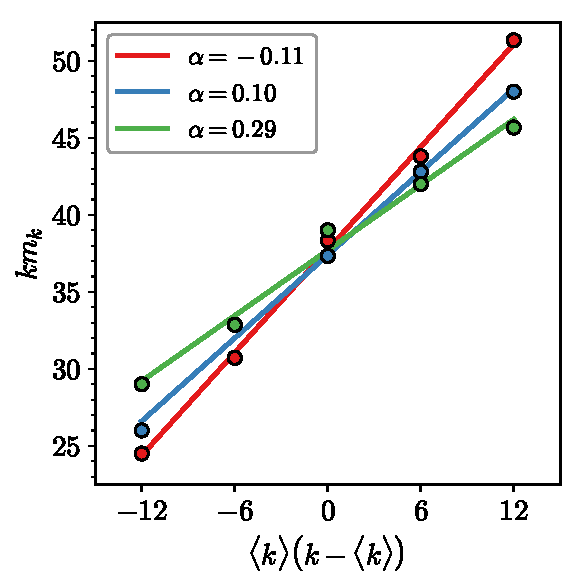
\includegraphics[width=8cm]{./figures/methods/aw_demo.pdf}
     \caption{Calculation of an \aw{} fit for three configurations (shown in figure \ref{fig:zach}(b)\--(d)). The value of the $\alpha$ parameter quantifies the tendency of small rings to be adjacent to large rings, with a larger value indicating stronger small\--large ring correlations.}
     \label{fig:awdemo}
\end{figure}

Despite the \aw{} law being purely empirical and there being no topological requirement for $m_k$ to vary systematically $k$, the law does seem to hold well for a diverse set of physical systems.
The law is well used for example in studies of materials, emulsions, biological tissues as well as in planetary science \cite{LeRoux2013,Roy2018,Noever1992,Mombach1993,Pedro2008}.
As an example of the calculation of the \aw{} parameter, the plots of the fits for the systems in figure \ref{fig:zach} are presented in figure \ref{fig:awdemo}, along with the corresponding $\alpha$ parameters.
This demonstrates two contrasting aspects of the \aw{} law. 
Firstly the law holds very well, especially given the fact that these samples consist of just twenty rings each.
However, it also demonstrates that the law is by no means exact and that some greyness is inevitably introduced during the linear regression.


\chapter{Computational Methods}
\label{ch:compmethods}

\begin{chapterabstract}
The theoretical basis of \mc{} methods and their application to generating realisations of \td{} networks is reviewed.
There is a broad discussion of Metropolis \mc{} methods, before specific methods are covered in detail; namely the bond switching algorithm and hard particle \mc{} in conjunction with the Voronoi construction.
Extensions to these methods and additional approaches are outlined in the relevant chapters \davidnote{Link to bond switching/Voronoi/mx2/procrystals later}.
\end{chapterabstract}

\section{General \mc{} Methods}
\label{sec:mc}

\mc{} methods are a class of computational algorithms designed to solve complex problems stochastically.
These normally fall into the broad categories of calculating integrals, sampling probability distributions and finding global minima of very high dimensional functions \-- tasks which are often incredibly hard to compute deterministically.
Since their initial development in the mid\--20\th{} century, such methods have become an invaluable tool for solving problems in the physical sciences.
\mc{} methods are used in this context for calculating thermodynamic averages of properties in equilibrium systems; finding the minima in potential energy surfaces of small molecules, glasses, crystals and biomolecules; as well as non\--equilibrium simulations such as growth of crystals and thin\--films \cite{Landau2014,Wales1999,Levi1997,Ratsch2003,Kob1999,Jensen1999}.
In this thesis these \mc{} methods  will be used in a variety of contexts chapter xxx \davidnote{fill this in}.
Therefore, the general theory is presented here with specific details of two established methods: bond switching and hard particle \mc{} given in the following section.

\subsection{Statistical Mechanics}

The total energy of a system with a fixed number of particles, $\mathcal{N}$, is given by the Hamiltonian,
\begin{equation}
	\ham = \ken+\pen \,,
\end{equation}
where $\ken$ is the kinetic energy as a function of all particle momenta and $\pen$ is the potential energy as a function of all particle positions \cite{Frenkel2002}.
The positions and momenta comprise the phase space of the system.
At fixed volume, $\mathcal{V}$, and temperature, $T$, all the the essential thermodynamic information is then provided through the classical canonical partition function:
\begin{equation}
	Q = \frac{1}{h^{D\mathcal{N}}\mathcal{N}!}\int \dd\mathbf{p}\,\dd\mathbf{r}\,\exp{\left[-\ham/ \kb T\right]}\,,
\end{equation}
where $D$ is the number of spatial dimensions.
This can be factorised into kinetic and potential components as
\begin{equation}
	Q = \frac{1}{h^{D\mathcal{N}}\mathcal{N}!}\int \dd\mathbf{p}\,\exp{\left[-\ken/\kb T\right]} \int \dd\mathbf{r}\,\exp{\left[-\pen/\kb T\right]} \,,
\end{equation}
where
\begin{equation}
	Z = \int \dd\mathbf{r}\,\exp{\left[-\pen/\kb T\right]}
\end{equation}
is the configurational integral \cite{Allen2017}. 
As will be shown, in \mc{} simulations it is the energetic differences between configurations that are required, and so at constant temperature the kinetic component can be neglected and it is only the configurational integral that is of importance.
In this case the probability density of the system being in the configuration $\mathbf{r}$ is given by the Boltzmann distribution:
\begin{equation}
	\label{eq:boltzmann}
	P\left(\mathbf{r}\right) = \frac{\exp{\left[-\pen/\kb T\right]}}{Z}\,.
\end{equation}
This allows the expectation value of an observable of the system, $\obs$, to be determined from:
\begin{equation}
	\label{eq:expectationobs}
	%\langle A \rangle = \frac{1}{Z}\int \dd\mathbf{r}\,\obs\exp{\left[-\pen/\kb T\right]} \,.
		\langle A \rangle = \int \dd\mathbf{r}\,\obs P\left(\mathbf{r}\right) \,.
\end{equation} 
The expectation value is then the ratio of two $\mathcal{N}D$ dimensional integrals.
The next section shows how these can be evaluated by \mc{} sampling.

\subsection{Importance Sampling}

An integral of form \eqref{eq:expectationobs} can be evaluated numerically by a number of methods.
As an illustration, consider the simple example of a \td{} potential energy surface in figure \ref{fig:montecarloint}.
To calculate the expectation value of the potential energy one must evaluate the integral
\begin{equation}
	\langle \mathcal{U} \rangle = \int_{0}^{L_y}\int_{0}^{L_x} \dd x \dd y\, \mathcal{U}\left(x,y\right)\mathcal{P}\left(x,y\right)\,.
\end{equation}
One way to achieve this would be to use standard numerical methods such as the trapezium rule or Simpson's rule to calculate the potential energy over a regular grid of points, as in figure \ref{fig:montecarloint1}, weighting each according to the Boltzmann distribution.

An alternative would be to take a stochastic approach.
In the simplest implementation, a series of $S$ random sampling points, $\left(x_i,y_i\right)$, can be generated uniformly in the intervals $\left[0,L_x\right]$ and $\left[0,L_y\right]$, as in figure \ref{fig:montecarloint2}.
Weighting these according to the Boltzmann distribution and averaging gives an estimation to the integral:
\begin{equation}
	\langle \mathcal{U} \rangle = \frac{L_xL_y}{S}\sum_{i=1}^{S} \mathcal{U}\left(x_i,y_i\right)\mathcal{P}\left(x_i,y_i\right)\,,
\end{equation}
which converges to the exact value as $S\rightarrow\infty$.

However, both quadrature and \mc{} uniform sampling suffer from the same inefficiency.
As can be seen in both schemes, many of the sampling points fall in regions of phase space where the potential energy is high and hence the weighting probability distribution is very small at reasonable temperatures.
In effect, significant effort is spent calculating regions where the contribution to the total integral is negligible.
A better approach is therefore to generate a series of $S$ random sampling points, $\left(x_i,y_i\right)$, according to the distribution $\mathcal{P}\left(x,y\right)$, as in figure \ref{fig:montecarloint2}.
The expectation value of the observable can then be calculated using a simple average:
\begin{equation}
	\langle \mathcal{U} \rangle = \frac{1}{S}\sum_{i=1}^{S} \mathcal{U}\left(x_i,y_i\right)\,.
\end{equation}
This is known as importance sampling and is vastly more efficient when dealing with an aggressive probability distribution like the Boltzmann, where only a small proportion of the phase space is accessible.

\begin{figure}[bt]
     \centering
     
     \begin{subfigure}[b]{0.45\textwidth}
         \centering
         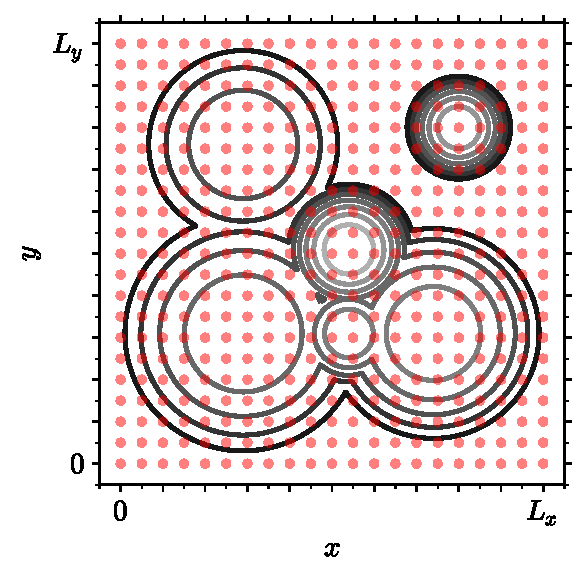
\includegraphics[width=\textwidth]{./figures/methods/mc_2d_quad.pdf}
         \caption{Quadrature.}
         \label{fig:montecarloint1}
     \end{subfigure}
     \hfill
     \begin{subfigure}[b]{0.45\textwidth}
         \centering
         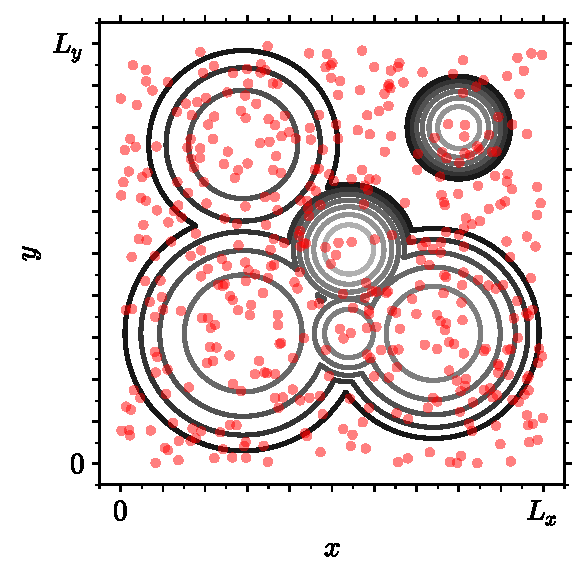
\includegraphics[width=\textwidth]{./figures/methods/mc_2d_rand.pdf}
         \caption{Uniform Sampling.}
         \label{fig:montecarloint2}
     \end{subfigure}
     \hfill
     
     \begin{subfigure}[b]{0.45\textwidth}
         \centering
         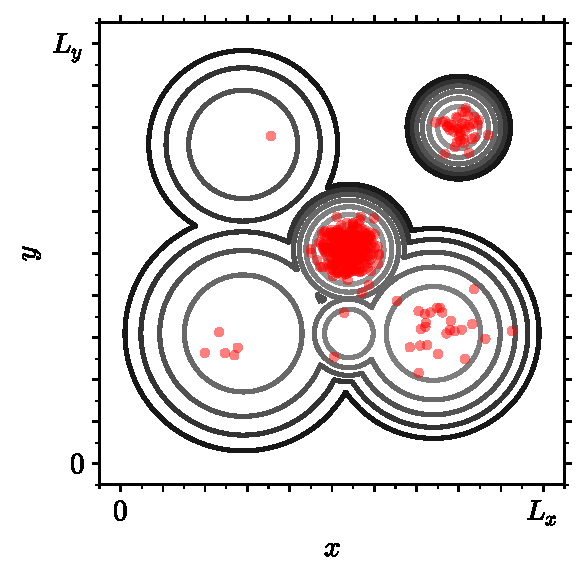
\includegraphics[width=\textwidth]{./figures/methods/mc_2d_imp.pdf}
         \caption{Importance Sampling.}
         \label{fig:montecarloint3}
     \end{subfigure}
     \hfill
     \begin{subfigure}[b]{0.45\textwidth}
         \centering
         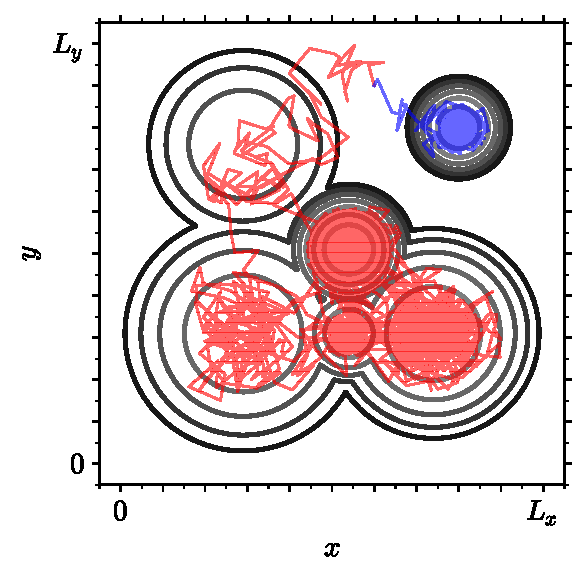
\includegraphics[width=\textwidth]{./figures/methods/mc_2d_mcmc.pdf}
         \caption{Markov Chain \mc}
         \label{fig:montecarloint4}
     \end{subfigure}
     \hfill
    
     \caption{Demonstration of different sampling methods with an example \td{} potential energy surface (contour lines). Panels(a)\--(c) display the same number of (red) sampling points. Panel (a) shows conventional quadrature where the surface is divided into a regular grid of sampling points which are then weighted by the Boltzmann distribution. Panel (b) shows \mc{} sampling with a uniform distribution of points which again must be Boltzmann\--weighted. Panel (c) shows \mc{} importance sampling with points now selected according to the Boltzmann distribution. Panel (d) shows Markov chain \mc{} with two random walks through phase space (red and blue lines) starting from different random seeds.}
     \label{fig:montecarloint}
\end{figure}

Whilst this scheme is ideal theoretically, it is impracticable for physical systems.
This is because for any problem of real interest one lives in a ``black box'' where the functional form of the potential energy surface in its hundreds if not thousands of dimensions is unknown.
In this case often the only way of learning about the form is by on\--the\--fly exploration of the surface \cite{Brooks2011}.
This can be achieved by talking a random walk through configurational space using Markov chain \mc.

\subsection{Markov Chain Monte Carlo}

Markov chain Monte Carlo provides a framework to perform importance sampling on a potential energy surface.
A system of interest can exist in a (very large) number of configurational states, $\left\{\mathbf{r}_0,\mathbf{r}_1,\dots,\mathbf{r}_M\right\}$.
A Markov chain can then be constructed from this set, whereby a sequence of states is generated stochastically across a series of steps, $s=0,1,\dots,S$.
In this process, the probability of moving between states at each step is given by the transition matrix, $\bm{\pi}$, where each element, $\pi_{ij}$, gives the probability of moving from the state $\mathbf{r}_i$ to another state $\mathbf{r}_j$.  
This leads to the two relationships:
\begin{align}
	0\leq \pi_{ij} &\leq 1\,, \\
	\sum_{j} \pi_{ij} &= 1\,, \label{eq:tmrowsum}
\end{align}
the first being a statement of the probabilistic nature of the elements whilst the second ensures all transfer remains within the state space \cite{Frenkel2002,Allen2017,Brooks2011}.

The probability that the system is in each state at a given step, $s$, can be represented by the row vector $\mathbf{P}_s$.
This probability distribution evolves with each step as $\mathbf{P}_{s+1}=\mathbf{P}_{s}\bm{\pi}$, so that starting from any initial distribution, $\mathbf{P}_0$, it follows that $\mathbf{P}_S=\mathbf{P}_0\bm{\pi}^S$. 
The question is then as to the behaviour as $S\rightarrow \infty$.
Provided certain criteria are met, the distribution will tend to a stationary distribution, $\mathbf{P}$, which satisfies the eigenvalue equation 
\begin{equation}
	\mathbf{P} = \mathbf{P}\bm{\pi}\,, \label{eq:mcmceig}
\end{equation}
regardless of the initial distribution (although the speed of the convergence does depend on $\mathbf{P}_0$).
This will occur only if the system is \textit{ergodic}, meaning that every state is connected to every other by some finite path.

In a discrete analogue to equation \eqref{eq:expectationobs}, the expectation value of an observable, $A$, can be calculated from the ensemble average:
\begin{equation}
	\langle A \rangle = \sum_{i=1}^{M} A\left(\mathbf{r}_i\right)\mathcal{P}\left(\mathbf{r}_i\right)\,,
\end{equation}
where $\mathcal{P}\left(\mathbf{r}_i\right)$ are the elements of $\mathbf{P}$.
However, as previously mentioned the number of discrete states is usually exceedingly large and so calculating the average over all states is not possible.
The solution is to take a random walk across through configurational space, sampling explicit states to form the chain $X_0,X_1,\dots,X_S$; where each move is chosen randomly according to the transition matrix $\bm{\pi}$.
In this case the expectation of the same observable can be calculated from the average over the sampled states:
\begin{equation}
	\langle A \rangle = \frac{1}{S}\sum_{i=1}^{S} A\left(X_i\right)\,,
\end{equation}
where the true value is approached as $S\rightarrow \infty$.

In this section the problem of sampling phase space efficiently has been reformulated, but as yet not solved. 
This is because the form of the transition matrix is still unknown.
Instead only the ideal form of the limiting probability distribution, $\mathbf{P}$, is available \-- where the elements follow the Boltzmann probabilities in equation \eqref{eq:boltzmann}.
A practical solution to this problem is provided by the Metropolis algorithm.

\subsection{Metropolis Algorithm}
\label{ssec:metropolis}

The Metropolis algorithm gives a prescription of how to construct a transition matrix, $\bm{\pi}$, with the requisite properties that samples the Boltzmann distribution \cite{Metropolis1953}.
Firstly, combining equations \eqref{eq:tmrowsum} and \eqref{eq:mcmceig} gives a condition on the transition matrix known as global balance:
\begin{equation}
	\sum_j \mathcal{P}\left(\mathbf{r}_i\right)\pi_{ij} = \sum_j \mathcal{P}\left(\mathbf{r}_j\right)\pi_{ji}\,.
\end{equation} 
Whilst it is possible to construct transition matrices which satisfy only global balance \cite{Manousiouthakis1999,Suwa2010,Michel2014}, it is practically simpler to satisfy global balance by applying the stronger condition of detailed balance:
\begin{equation}
	\mathcal{P}\left(\mathbf{r}_i\right)\pi_{ij} = \mathcal{P}\left(\mathbf{r}_j\right)\pi_{ji}\,.
\end{equation}
In the Metropolis algorithm the off\--diagonal elements of the transition matrix are written as the product of two probabilities: 
\begin{equation}
	\pi_{ij} = \begin{cases} 
		\tau_{ij}P_{ij} \quad & i\neq j \\
		1-\sum\limits_{j\neq i}\tau_{ij}P_{ij} \quad & i=j
	\end{cases}\,,
\end{equation}
where $\tau_{ij}$ is the trial probability of moving from state $\mathbf{r}_i$ to $\mathbf{r}_j$ and $P_{ij}$ is the probability of accepting the trial move.
To conform to detailed balance, the trial probabilities must be chosen to satisfy $\tau_{ij}=\tau_{ji}$.
Then, in the crux of the algorithm, the acceptance probabilities are given by
\begin{align}
	 P_{ij}&=\begin{cases}
	 	1 \quad &\mathcal{P}\left(\mathbf{r}_j\right)\geq \mathcal{P}\left(\mathbf{r}_i\right) \\
	 	\frac{\mathcal{P}\left(\mathbf{r}_j\right)}{\mathcal{P}\left(\mathbf{r}_i\right)} \quad & \mathcal{P}\left(\mathbf{r}_j\right)< \mathcal{P}\left(\mathbf{r}_i\right)
	 \end{cases}
	 =\begin{cases}
	 	1 \quad &\mathcal{U}\left(\mathbf{r}_j\right)\leq \mathcal{U}\left(\mathbf{r}_i\right) \\
	 	\frac{\exp\left[-\mathcal{U}\left(\mathbf{r}_j\right)/\kb T\right]}{\exp\left[-\mathcal{U}\left(\mathbf{r}_i\right)/\kb T\right]} \quad & \mathcal{U}\left(\mathbf{r}_j\right)>\mathcal{U}\left(\mathbf{r}_i\right)
	 \end{cases}\,,
\end{align}
which can be expressed more succinctly as
\begin{equation}
	\label{eq:metropolis}
	 P_{ij}=\text{min}\big[1,\exp\left[-\Delta \mathcal{U}/\kb T\right]\big]\,,
\end{equation}
where $\Delta \mathcal{U}$ is the difference in potential energy between the final and initial states.
The elegance of the Metropolis algorithm lies in the fact that the acceptance probability depends only on the ratio of the configuration probabilities removing the need for a normalising factor.
This means the relative probabilities can be used (which are computable) instead of the absolute probabilities (which are unknowable).

The final stage is the choice of the matrix of trial probabilities, $\bm{\tau}$. 
This is very flexible and one can be creative in the selection of trial moves, providing that the underlying matrix is symmetric and ergodic.
An effective strategy is to choose moves in which the trial state is relatively close to the current state to trace the paths of high probability in the system.
A summary of the Metropolis algorithm is therefore as follows:
\begin{enumerate}
	\item Initialise the system in a state $X_{s=0}$ and calculate the potential energy $\mathcal{U}\left(X_s\right)$
	\item Generate a trial state $X_t$ (a perturbation of $X_s$) according to $\tau_{st}$
	\item Calculate the potential energy of the trial state $\mathcal{U}\left(X_t\right)$
	\item Determine acceptance or rejection of the trial move according to the Metropolis criterion \eqref{eq:metropolis}
	\item Update the system to the new state: if the trial move is accepted $X_{s+1}=X_{t}$ otherwise $X_{s+1}=X_{s}$
	\item Repeat steps 2\--5
\end{enumerate}
There are a few practical factors related to the scheme above.
In Markov chain \mc{} it was previously mentioned that it takes time for the system to evolve to the stationary distribution.
Therefore it is necessary to have an equilibration period where the chain is generated but not used for sampling of observables.
In addition, whilst selecting trial moves close to the current state increases efficiency, it introduces correlation into the procedure.
A way around this is to not calculate observables based on every step, but rather after a number of statistically significant steps.

As an example of the Metropolis algorithm, consider again the \td{} potential energy surface in figure \ref{fig:montecarloint4}.
Here two simulation paths are displayed in red and blue, starting from the same initial state but with different starting points in the random number generators \ie{} random seeds.
As can be seen the Metropolis algorithm takes a random walk over the configurational space, conducting importance sampling as in \ref{fig:montecarloint3}.
However, in this example highlights a potential problem.
There are two regions of phase space with non\--zero probabilities which are separated by a relatively large energy barrier.
Although they are in principle linked by a path, the barrier may effectively mean they are disconnected on a reasonable simulation time scale, breaking ergodicity.
This manifests as the red walk sampling one region and the blue walk being trapped in the other region.
Using multiple seeds in this way helps to identify if any such behaviour is present.
If it leads to significant differences in the computed averages, more advanced techniques using enhanced sampling may have to be employed \cite{Torrie1977,Earl2005}.

\subsection{Global Optimisation \& Simulated Annealing}
\label{s:simulatedannealing}

So far in this section it has been shown how Monte Carlo methods can be used perform importance sampling of potential energy surfaces.
These methods can also be used to solve the related problem of finding global minima in potential energy surfaces and other more general functions.
Consider the case where there is an objective function, $\obj\left(\mathbf{r}\right)$, which depends on particle positions.
If it is known that there exists a solution where $\obj\left(\mathbf{r}\right)=0$, it may be sufficient to perform a standard random walk of the type in figure \ref{fig:montecarloint4} until a solution is found, using the more general Metropolis criterion:
\begin{equation}
	\label{eq:objmetropolis}
	P_{ij} = \min\big[1,\exp\left[-\Delta\Omega/\kb T\right]\big].
\end{equation}
There is of course a chance that the optimisation will not converge to the global minimum, most likely getting trapped in a local minimum (as for instance the blue path in \ref{fig:montecarloint4}).
One solution to this problem is just to keep restarting the algorithm with different initial conditions until the global minimum is obtained.

Often however the value of the global minimum is not known, as is the case for a potential energy surface, and this rudimentary approach is insufficient.
One must then employ a more sophisticated technique to find the global minimum of a very high dimensional and potentially rough surface.
This in itself is an extensive area of study and there are many approaches such as using genetic algorithms or basin\--hopping \cite{Hartke1993,Niesse1996,Wales1997}.
This thesis will use simulated annealing, which can be considered an extension to Metropolis \mc{} \cite{Kirkpatrick1983}.
In addition simulated annealing is effective for searching surfaces with many similar minima as in glasses \-- the name reflecting its origins in the analogous process in metallurgy to generate defect free metals.

\begin{figure}[tb]
     \centering
    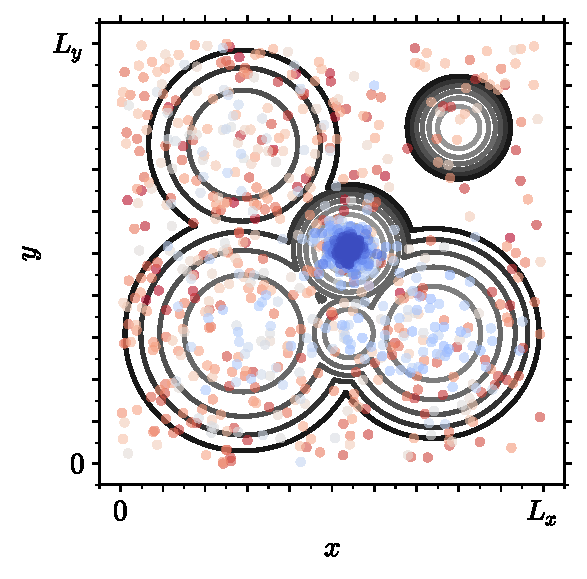
\includegraphics[width=0.45\textwidth]{./figures/methods/mc_2d_sa.pdf}
      \caption{Demonstration of the simulated annealing algorithm on a \td{} potential energy surface, with states coloured by temperature (red$\rightarrow$blue indicating hot$\rightarrow$cold. As the temperature is reduced the state converges on the global minimum.}
      \label{fig:montecarloint5}
\end{figure}

The simulated annealing algorithm proceeds as follows.
The system of interest is first thermalised by performing Metropolis \mc{} at infinite temperature \ie{} accepting every move. 
The system is then gradually cooled to zero temperature, with the Metropolis criterion \eqref{eq:objmetropolis} reducing the proportion of accepted moves.
In theory if the cooling is infinitely slow, the system is maintained in thermal equilibrium and will eventually reach the global minimum \cite{Henderson2003}.
In practice this is not realisable and so a cooling rate must be empirically selected.
Still it is possible for trapping to occur in local minima, especially if the transition between low energy states is very slow.
As before, one can then cycle the simulated annealing, repeatedly heating and cooling the system until the global minimum is found.
The simulated annealing algorithm is demonstrated with the \td{} potential energy surface in figure \ref{fig:montecarloint5}.
As can be seen at high temperature the entire surface is sampled, overcoming all energy barriers, but as cooling takes place the system settles into the low energy regions of the surface, finally terminating in the global minimum.

\section{Bond Switching Monte Carlo}
\label{s:bondswitch}

Bond switching Monte Carlo was originally developed by Wooten, Winer and Weaire to generate high quality configurations of three dimensional silica glass \cite{Wooten1985}.
The basic principle is to amorphise a crystalline lattice with a series of transformations that swap the nearest neighbours of pairs of atoms and optimise the resulting structure to generate a continuous random network which is well\--relaxed.
These continuous random network models replicate experimental observables with high accuracy (including bond length and angle distributions, radial distribution functions, electronic band gaps and Raman spectra) and have since been applied to alternative systems such as three\--dimensional amorphous carbon, binary glasses and biological polymers \cite{Treacy2012,Tu1998,Djordjevic1995,Mousseau2004,Huisman2008,Broedersz2014}.
However, the method can also be readily modified to study \td{} systems, as has been done for amorphous graphene and silica, and which forms the basis for much of the work in this thesis \davidnote{ref to later chapters} \cite{Kumar2014,Jain2018}.
The basic algorithmic details are described in this section, with extensions given in sections \davidnote{again ref later}.

\subsection{Algorithmic Details} 

The \td{} bond switching algorithm essentially follows the prescription of simulated annealing in section \ref{s:simulatedannealing}.
A skeleton algorithm structure is outlined below, followed by specific details \cite{Kumar2012}.
Visualisations are provided for reference in figure \ref{fig:bsmc}.

\begin{enumerate}
	\item Generate initial crystalline hexagonal lattice
	\item Thermalise the lattice with a large number of random moves 
	\item Sample configurations by annealling the system slowly at finite temperature, accepting moves according to the Metropolis criterion \ref{eq:metropolis}
\end{enumerate}
\begin{figure}[bt]
     \centering
     
     \begin{subfigure}[b]{0.24\textwidth}
    \centering
         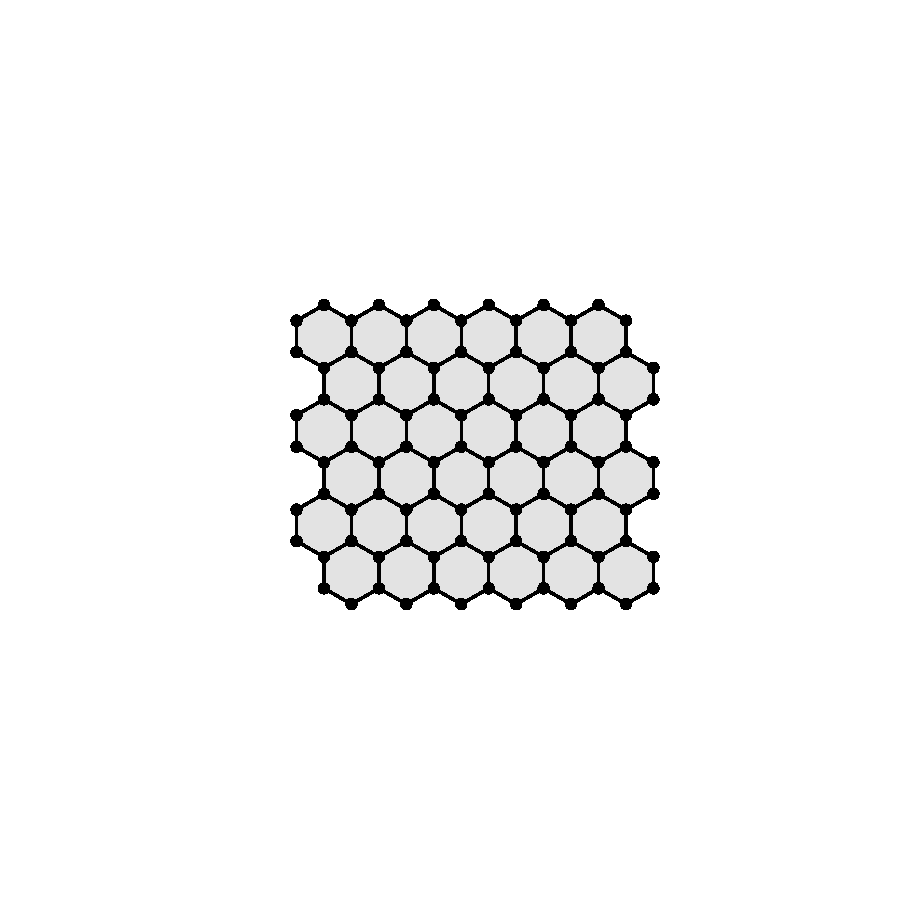
\includegraphics[height=2.8cm]{./figures/methods/bs_0.pdf}
         \caption{}
         \label{fig:bsmc1}
     \end{subfigure}
     \hfill
     \begin{subfigure}[b]{0.24\textwidth}
    \centering
         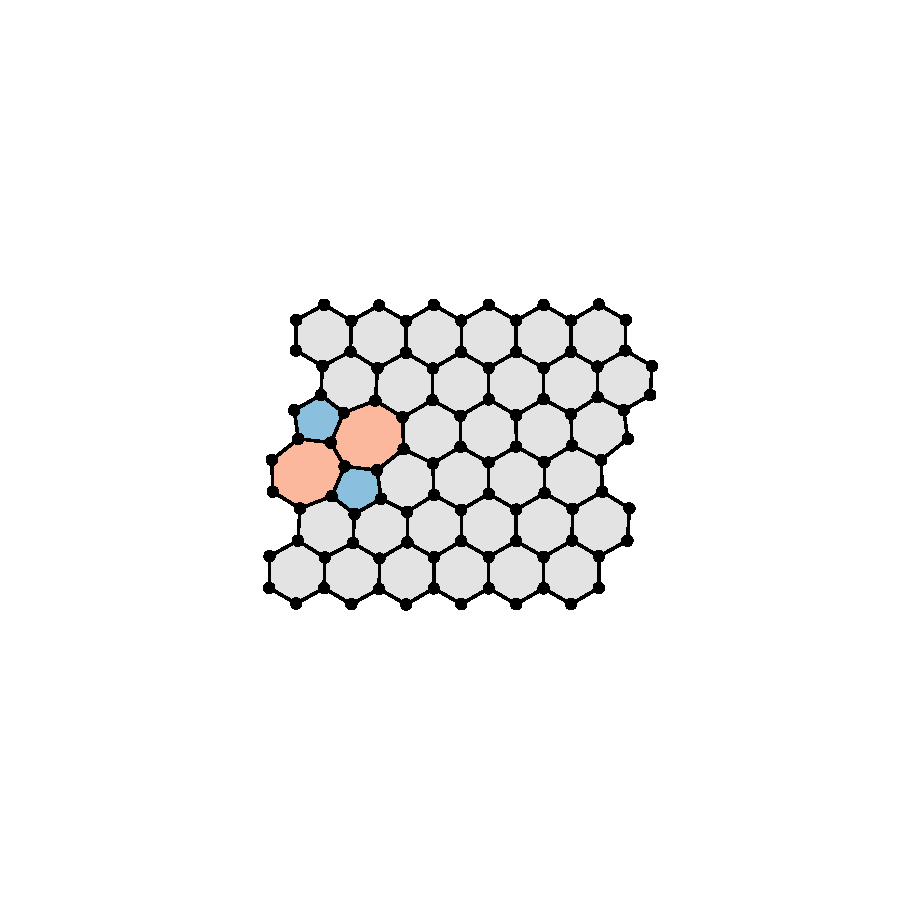
\includegraphics[height=2.8cm]{./figures/methods/bs_1.pdf}
         \caption{}
         \label{fig:bsmc2}
     \end{subfigure}
     \hfill
     \begin{subfigure}[b]{0.24\textwidth}
    \centering
         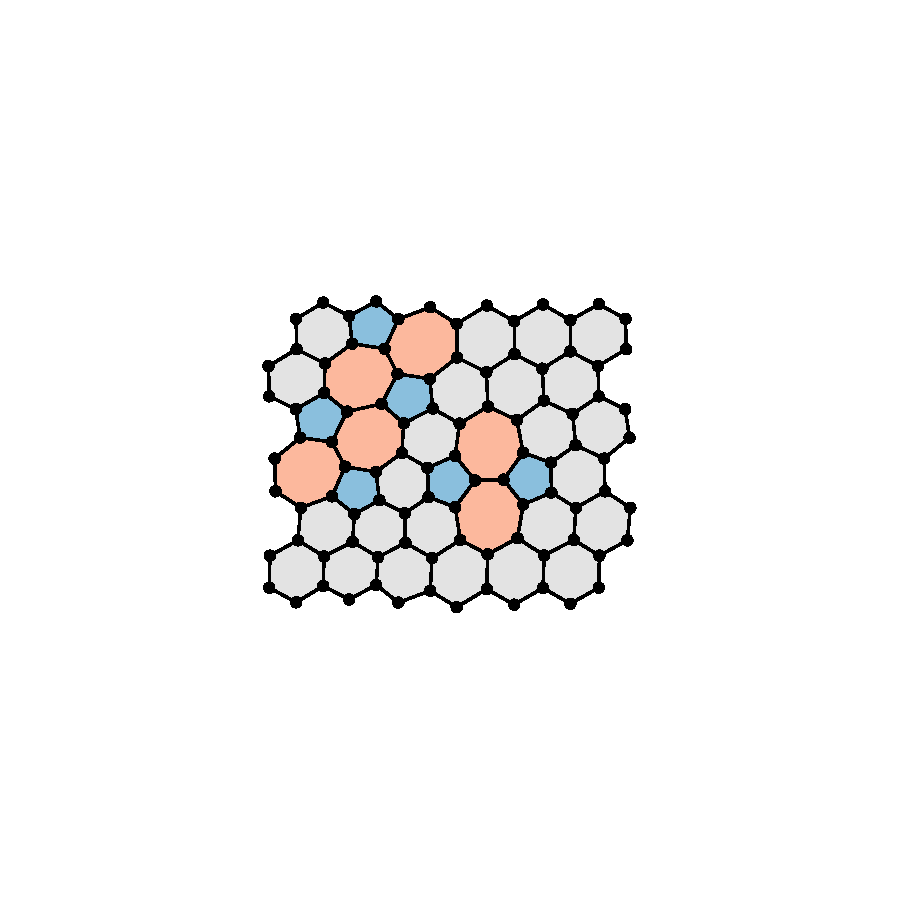
\includegraphics[height=2.8cm]{./figures/methods/bs_3.pdf}
         \caption{}
         \label{fig:bsmc3}
     \end{subfigure}
     \hfill
     \begin{subfigure}[b]{0.24\textwidth}
    \centering
         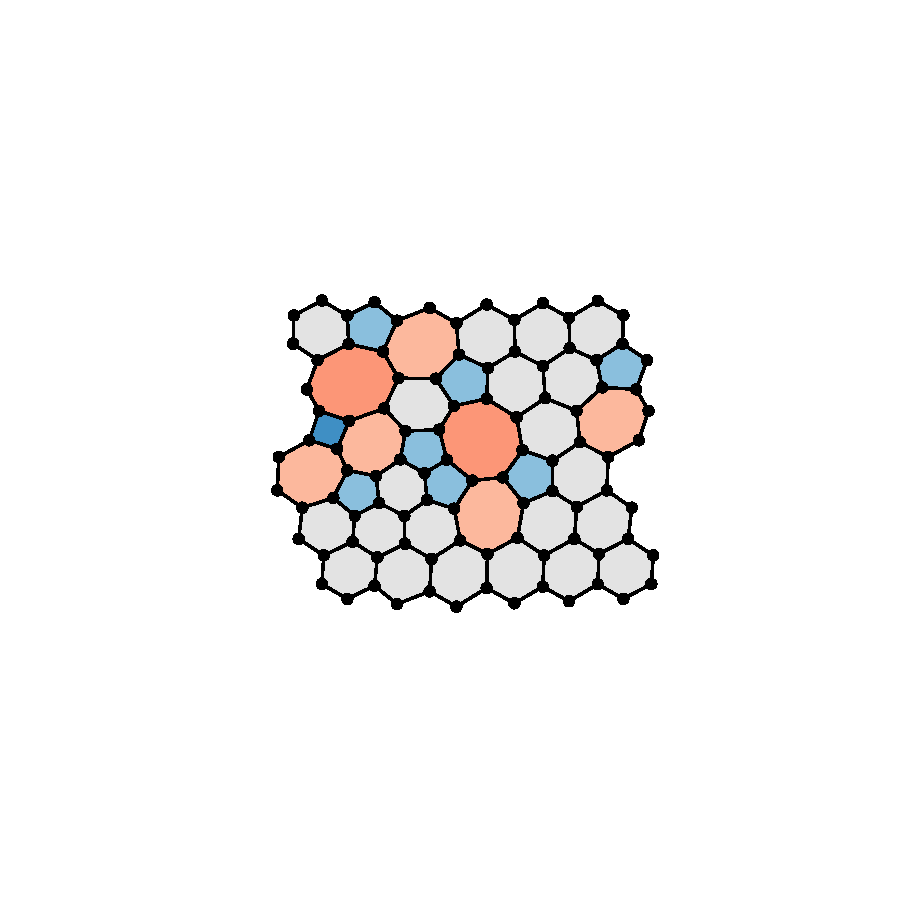
\includegraphics[height=2.8cm]{./figures/methods/bs_5.pdf}
         \caption{}
         \label{fig:bsmc4}
     \end{subfigure}
     
     \begin{subfigure}[b]{0.24\textwidth}
     \centering
         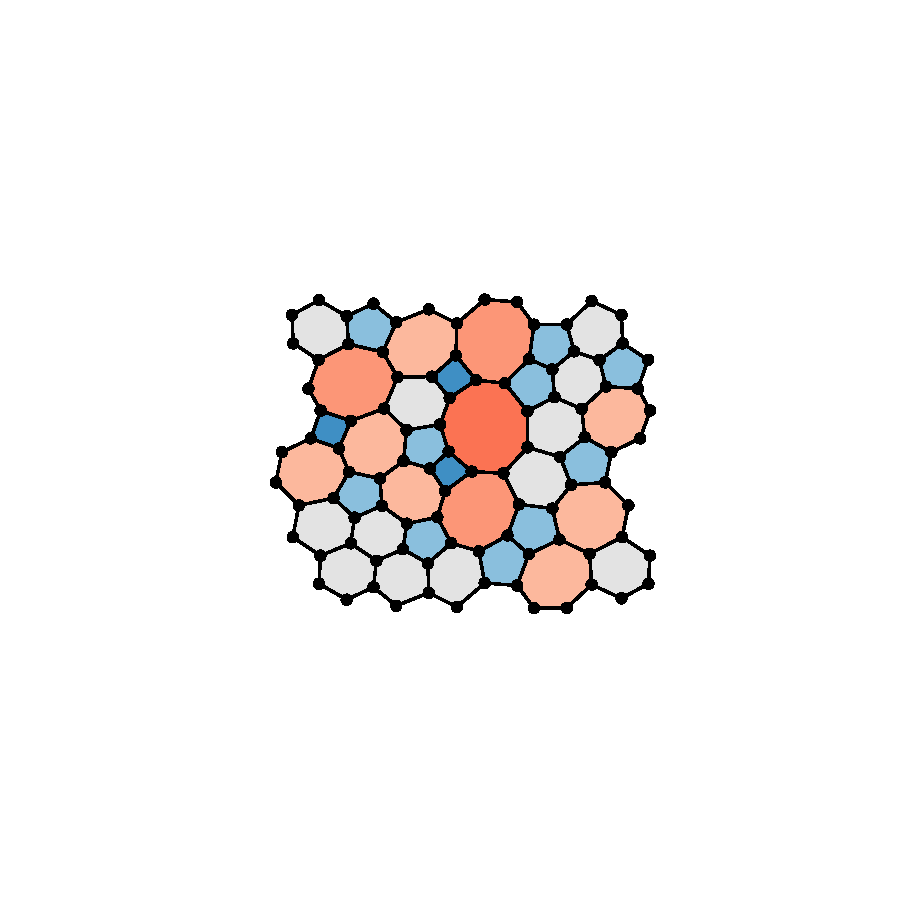
\includegraphics[height=2.8cm]{./figures/methods/bs_10.pdf}
         \caption{}
         \label{fig:bsmc5}
     \end{subfigure}
     \hfill
        \begin{subfigure}[b]{0.24\textwidth}
    \centering
         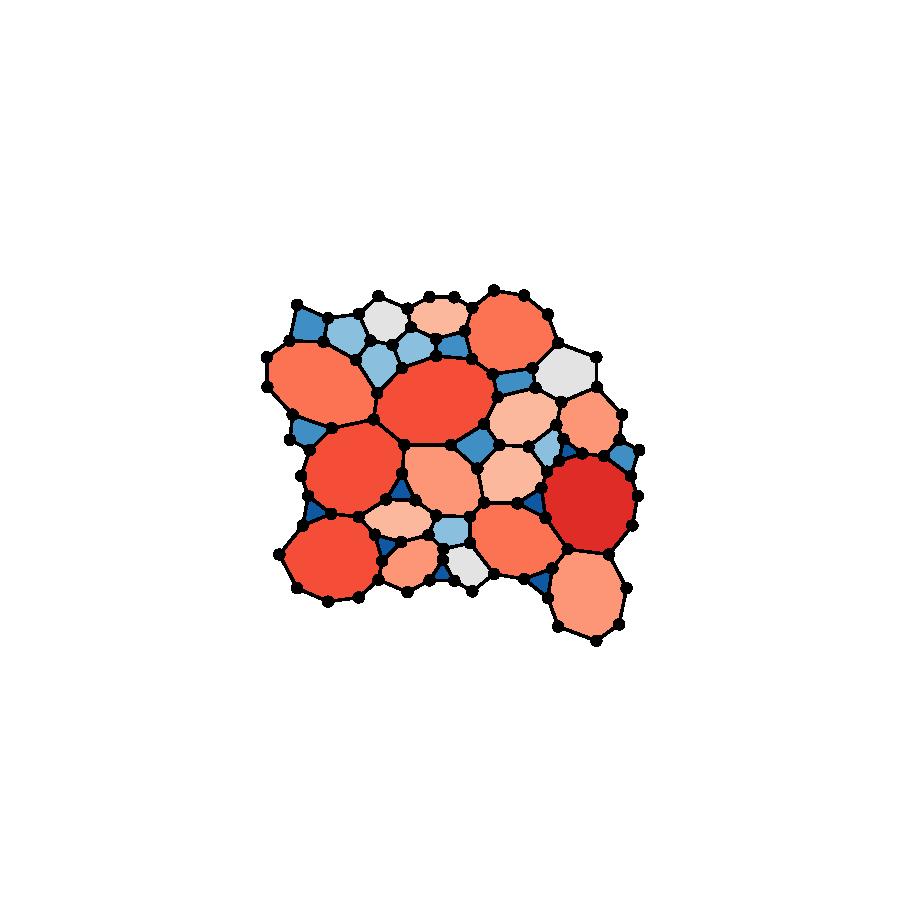
\includegraphics[height=2.8cm]{./figures/methods/bs_1000.pdf}
         \caption{}
         \label{fig:bsmc6}
     \end{subfigure}
     \hfill
           \begin{subfigure}[b]{0.24\textwidth}
    \centering
         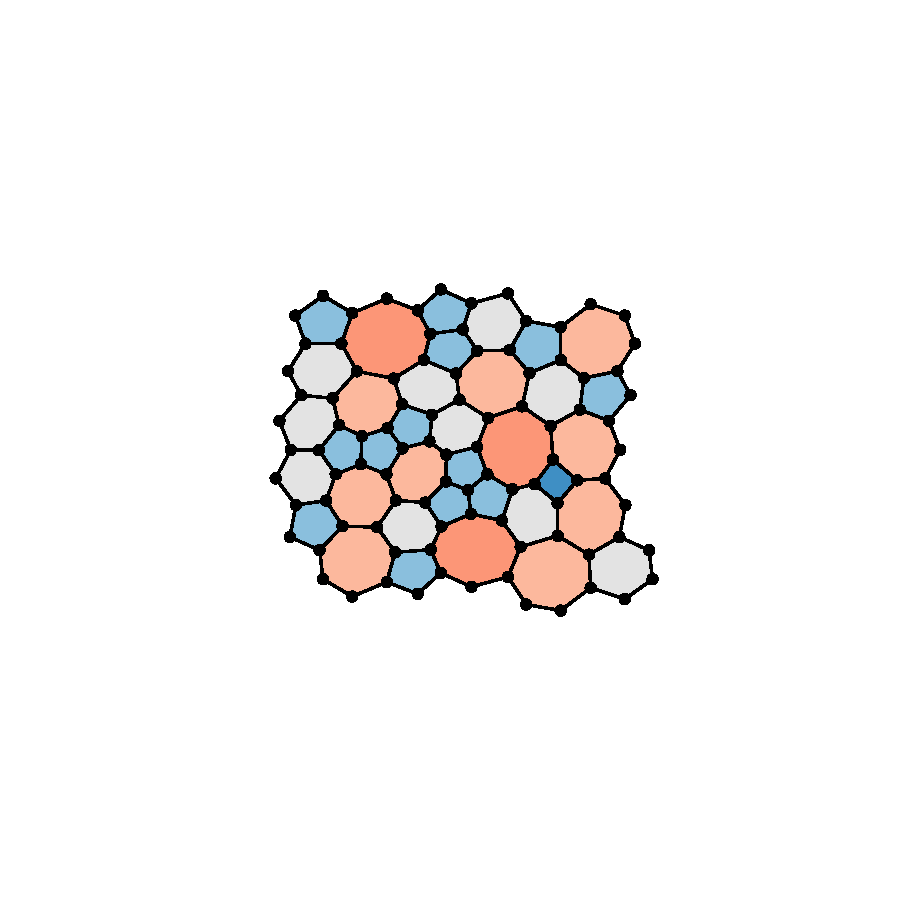
\includegraphics[height=2.8cm]{./figures/methods/bs_t1.pdf}
         \caption{}
         \label{fig:bsmc7}
     \end{subfigure}
     \hfill
           \begin{subfigure}[b]{0.24\textwidth}
    \centering
         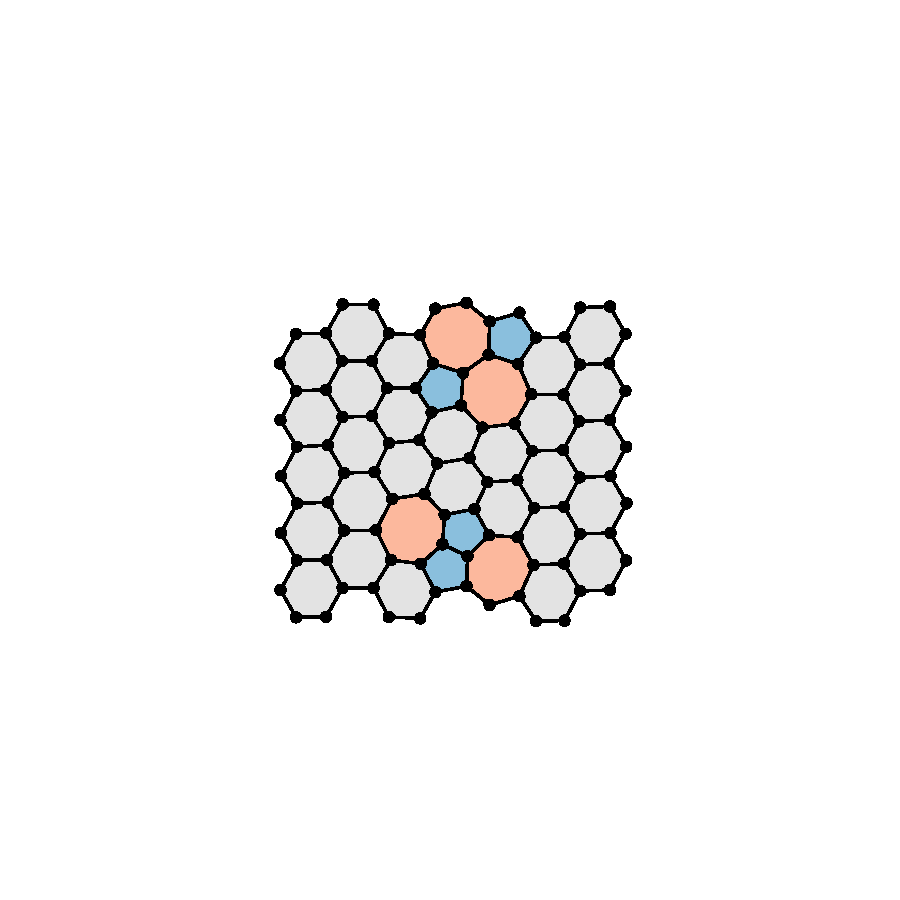
\includegraphics[height=2.8cm]{./figures/methods/bs_t2.pdf}
         \caption{}
         \label{fig:bsmc8}
     \end{subfigure}
   
     \caption{Configurations taken from stages of the \td{} bond switching algorithm. A crystalline lattice (a) is first thermalised to generate a random high energy network (f) by sequential overlapping Stone\--Wales defects (b)-(e). Sampling then occurs as the system is slowly annealed (g)-(h), allowing access to defect states that are not initially obtainable from the crystal structure.}
     \label{fig:bsmc}    
\end{figure}
The \mc{} move for 3\--coordinate atomic materials is essentially the introduction of a Stone\--Wales defect into the lattice, which
augments the size of two rings and decrements two others, preserving both the mean ring size and the coordination number of the individual atoms involved in the transformation \cite{Stone1986}.
As defects become more concentrated they overlap, leading to increasing diversity into the ring structure (allowing access to more than the pentagons and heptagons in a single Stone\--Wales defect).
Each bond transposition is followed by geometry optimisation to minimise and calculate the total energy of the system.  
A key aspect in the bond switching algorithm is therefore the choice of potential model.
The potential models and geometry optimisation process used in this thesis can be found in subsections below.

Cooling the system slowly ensures that the material remains in thermodynamic equilibrium, allowing configurations to be sampled throughout the simulation.
The ring structure of the system is then related to the temperature parameter, with more extreme ring sizes appearing at higher temperatures (compare figure \ref{fig:bsmc6}\--\ref{fig:bsmc8}).
This simply reflects the inherent balance of enthalpic \vs{} entropic  considerations.
Figure \ref{fig:bsmc8} also demonstrates the importance of cooling a randomised lattice instead of heating a crystal, as some low energy defects may have a multi\--step formation with a high energy barrier.  

\subsection{Potential Models}
\ref{s:potentials}

The nature of the bond switching method lends itself to the use of semi\--empirical potentials which have explicit stretching and angular neighbour lists.
As such a popular choice for materials modelling is the Keating potential and modifications thereof \cite{Keating1966,Barkema2000}. 
For a \td{} system the Keating potential has the form:
\begin{equation}
	\label{eq:keating}
	\pen = \frac{3}{16}\frac{\fk_S}{r_0^2}\sum_{\substack{i,j \in \\ \text{stretches}}} \left(r_{ij}^2-r_0^2\right)^2+
	\frac{3}{8}\frac{\fk_A}{r_0^2}\sum_{\substack{ijk \in \\ \text{angles}}}\left(r_{ij}r_{ik}\cos\theta_{ijk}-r_0^2\cos\theta_0\right)^2 \,,
\end{equation}
where $r_{ij}$ the distance and $\theta_{ijk}$ the angle between particles; whilst $\fk_S$ and $\fk_A$ are the force constants for the stretching and angular terms respectively \cite{Kumar2012}.
This potential drives the system towards equilibrium values of $r_0$ for the bond lengths and $\theta_0$ for the bond angles.
The Keating potential has been parametrised for a range of specific materials \cite{Kumar2012,Drabold2009}. 

However, a more generic potential model is sometimes required which captures the same essential physics.
This is provided through the simplified Keating potential \cite{VonAlfthan2003},
\begin{equation}
	\pen = \frac{\fk_S}{2}\sum_{\substack{i,j\in \\ \text{stretches}}}\left(r_{ij}-r_0\right)^2 + \frac{\fk_A}{2}\sum_{\substack{i,j,k \in \\ \text{angles}}} \left(\cos\theta_{ijk}-\cos\theta_0\right)^2\,,
\end{equation}
which is harmonic in stretching and angular terms.
One final modification can be made to this potential. 
Sometimes it is informative build models which enforce ring convexity \ie{} maintain all angles within the range $0\leq \theta_{ijk} \leq \pi$.
This can be achieved by augmenting the simplified Keating potential with a restricted bending (ReB) potential \cite{Bulacu2013}:
\begin{equation}
	\pen = \frac{\fk_S}{2}\sum_{\substack{i,j\in \\ \text{stretches}}}\left(r_{ij}-r_0\right)^2 + \frac{\fk_A}{2}\sum_{\substack{i,j,k \in \\ \text{angles}}} \frac{\left(\cos\theta_{ijk}-\cos\theta_0\right)^2}{\sin^{2}\theta_{ijk}}\,.
\end{equation}
The addition of the sine term in denominator causes the potential to diverge as bond angles approach linearity, preventing bonds from ``inverting''.

\subsection{Geometry Optimisation}
\label{s:geomopt}

The purpose of geometry optimisation is to minimise the overall potential energy of a network, $\pen$, as a function of all atomic positions, $\mathbf{r}$, after they have been perturbed \eg{} by a bond transposition.
As all initial configurations are well relaxed and perturbations relatively small, this can be achieved with a local minimisation routine.
In addition as the potential models in this work are smooth and harmonic, a straightforward steepest descent algorithm is both sufficient and efficient.

The steepest descent algorithm is an iterative method which searches down the potential energy gradient until a minimum is reached \cite{Nocedal2006}.
It has the following scheme:
\begin{enumerate}
	\item Calculate the potential energy of the system $\mathcal{U}_i=\mathcal{U}\left(\mathbf{r}_i\right)$
	\item Determine the negative gradient of the potential \ie{} the forces acting on the particles $\mathbf{F}_i=-\nabla \mathcal{U}_i$ 
	\item Find the optimal distance to displace the particles along the lines of force $\mathcal{U}_{i+1}=\min \left[\mathcal{U}\left(\mathbf{r}_i+\lambda \mathbf{F}_i\right)\right]$
	\item Set $\mathbf{r}_{i+1}=\mathbf{r}_i+\lambda_{\text{min}} \mathbf{F}_i$
	\item Evaluate convergence and repeat steps 1-4 if $\left|\mathcal{U}_{i+1}-\mathcal{U}_i\right|>\gamma$
\end{enumerate}
The calculation of forces in stage 2 will depend on the potential model used, details of which are given in appendix \ref{app:forces}.
Note that stage 3 also requires a minimisation routine, which may seem counter\--intuitive. 
However, this is a one\--dimensional minimisation which trivial to estimate with a line search method \davidnote{appendix?}.
The tightness of the convergence condition is set through the parameter $\gamma$.

One final performance improvement arises from the fact that the \mc{} are inherently local.
Therefore geometry optimisation can be employed such that only the atoms in the immediate vicinity of the switching move need to be minimised to obtain an accurate structure.
Typically this would extend to all atoms within five coordination shells of those directly involved in the switch move \cite{Mousseau2001}.

\section{Hard Particle \mc}
\label{s:hardparticlemc}

Hard particle Monte Carlo is one of the most well\--established computational methods in statistical physics.
Through its simplicity it is able to provide insight into the fundamental behaviour of particle systems and simulations of increasing size are still performed this century \cite{Isobe2016,Bernard2009,Anderson2013,Isobe2015}.
In this thesis it will be used to generate ring systems in the form of Voronoi tessellations (see section \ref{ssec:voronoi}), in analogy to experimental colloidal systems \cite{Thorneywork2017}.

\subsection{Hard Particle Model}

Hard particle models are applicable over a range of dimensions.
In two dimensions the system consists of an arrangement of hard disks and in three dimensions hard spheres.
One can also take a quasi \td{} system, which comprises hard spheres confined to a plane.
Regardless of the dimensionality, the central principle is that no two particles in the system can have any degree overlap.
Formally, if the particle radii are denoted by $R_i$ and the distance between any pair of particle centroids by $r_{ij}$, the pair potential is:
\begin{equation}
	\mathcal{U}_{ij} = \begin{cases}
	\infty \quad &r_{ij}<R_i+R_j \\
	0 \quad &r_{ij}\geq R_i+R_j 
	\end{cases} \,.
\end{equation}
As the total energy is simply then
\begin{equation}
	\pen = \sum_{i<j} \mathcal{U}_{ij}\,,
\end{equation}
it follows that if any pair of particles have overlap the system energy is infinite and the Boltzmann weighting is zero.
Hard particle models are typically quantified in terms of the packing fraction, $\phi$, which in two dimensions has the form
\begin{equation}
	\label{eq:packingfraction}
	\phi_{2D} = \rho\pi\langle R^2\rangle\,,
\end{equation}
where $\rho=\mathcal{N}/{V}$, the number density.

\subsection{Algorithmic Details} 

\begin{figure}[bt]
     \centering
     
     \begin{subfigure}[b]{0.25\textwidth}
         \centering
         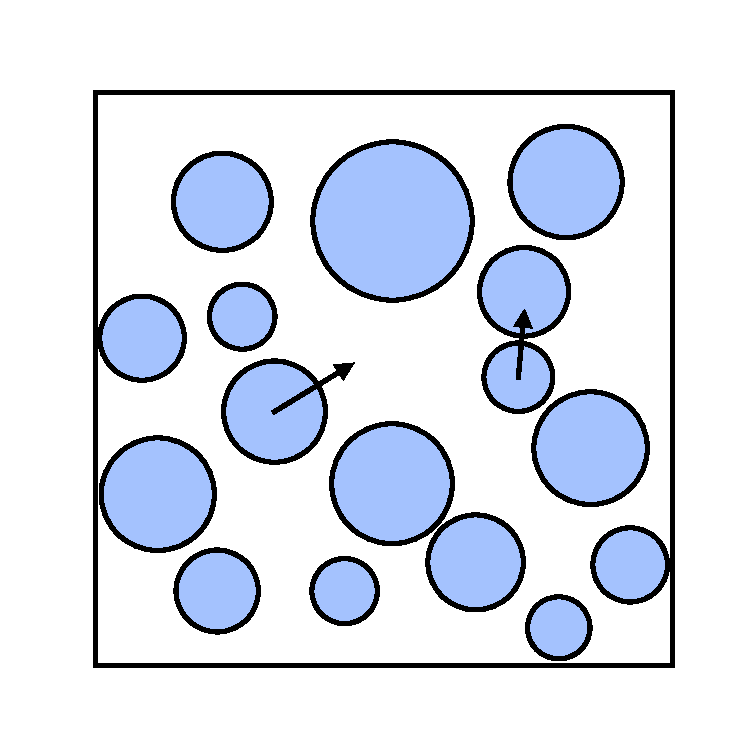
\includegraphics[width=3cm]{./figures/methods/mc_move_a.pdf}
         \caption{}
         \label{fig:hardmc1}
     \end{subfigure}
     \begin{subfigure}[b]{0.25\textwidth}
         \centering
         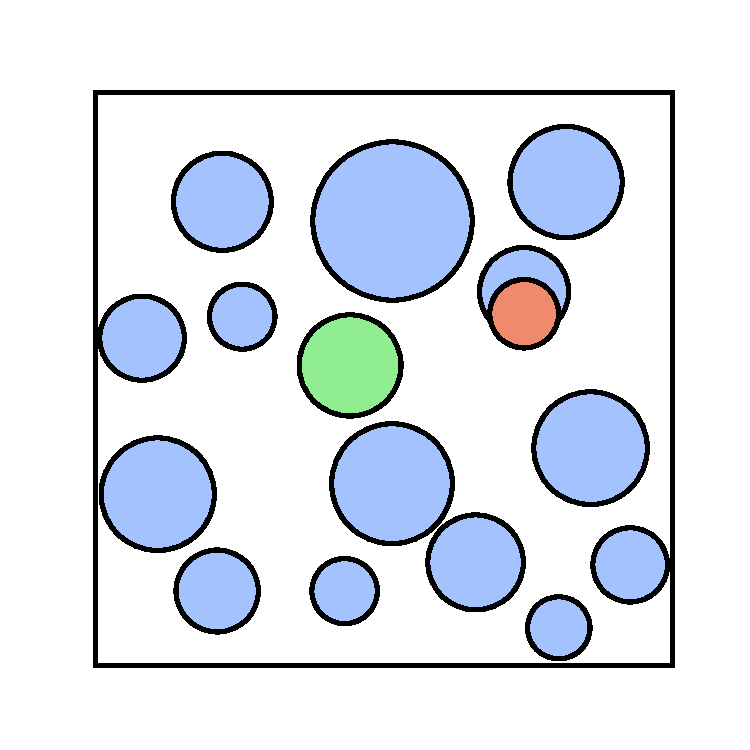
\includegraphics[width=3cm]{./figures/methods/mc_move_b.pdf}
         \caption{}
         \label{fig:hardmc2}
     \end{subfigure}
     \begin{subfigure}[b]{0.25\textwidth}
         \centering
         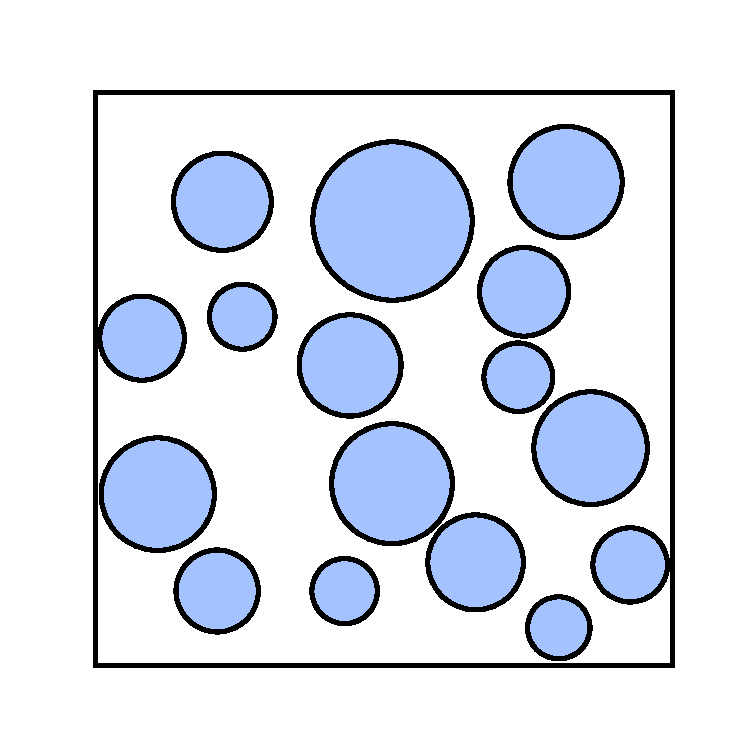
\includegraphics[width=3cm]{./figures/methods/mc_move_c.pdf}
         \caption{}
         \label{fig:hardmc3}
     \end{subfigure}
     
       \begin{subfigure}[b]{0.25\textwidth}
         \centering
         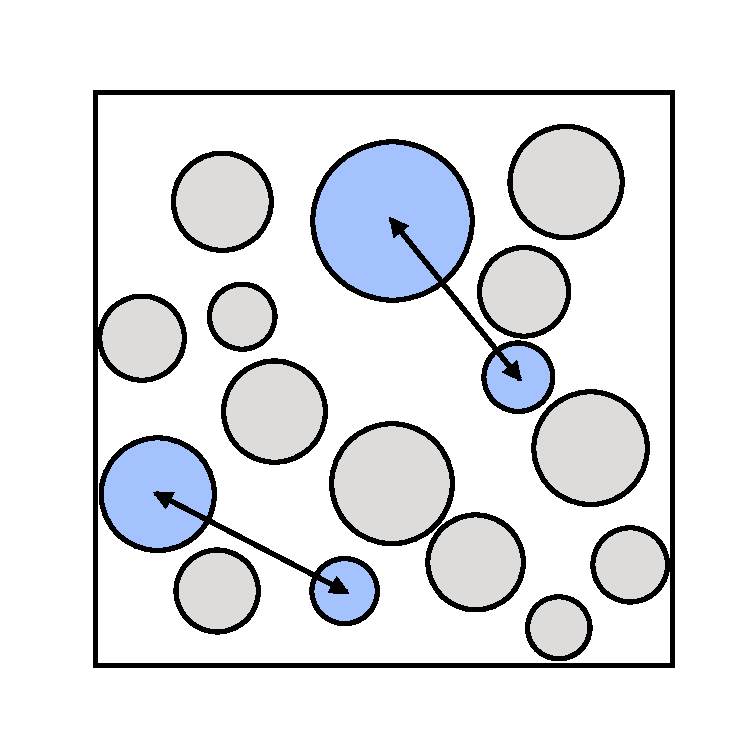
\includegraphics[width=3cm]{./figures/methods/mc_move_d.pdf}
         \caption{}
         \label{fig:hardmc4}
     \end{subfigure}
     \begin{subfigure}[b]{0.25\textwidth}
         \centering
         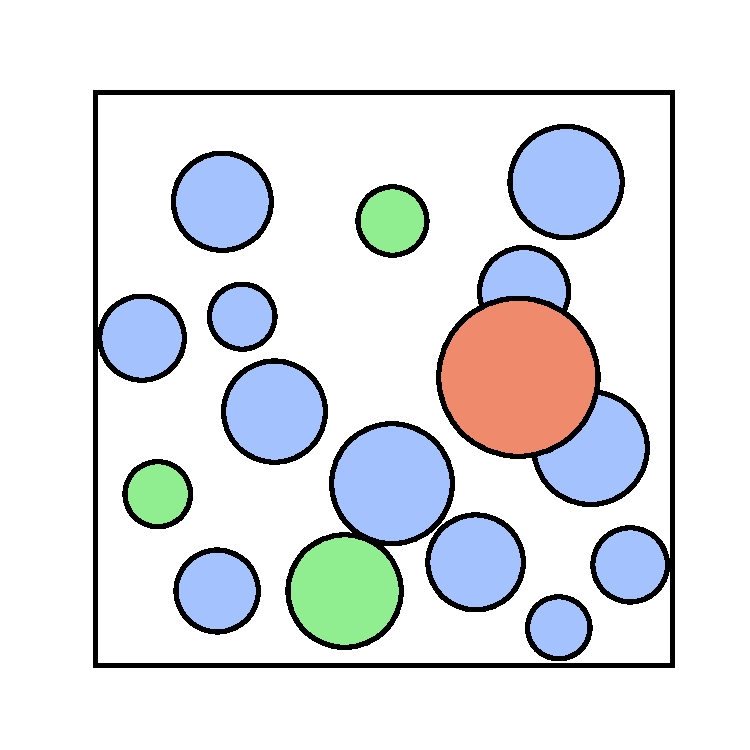
\includegraphics[width=3cm]{./figures/methods/mc_move_e.pdf}
         \caption{}
         \label{fig:hardmc5}
     \end{subfigure}
     \begin{subfigure}[b]{0.25\textwidth}
         \centering
         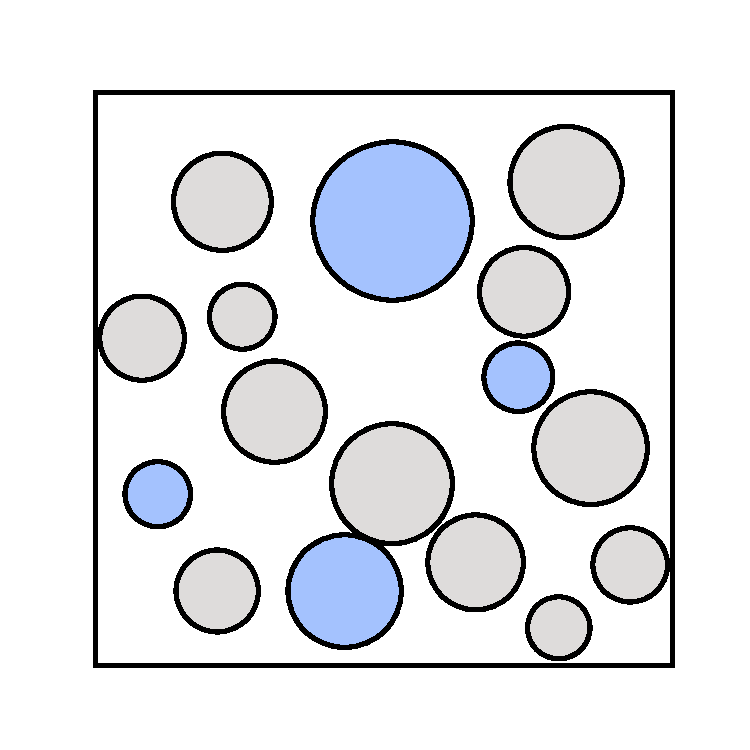
\includegraphics[width=3cm]{./figures/methods/mc_move_f.pdf}
         \caption{}
         \label{fig:hardmc6}
     \end{subfigure}
   
     \caption{Demonstration of two displacement (a)\--(c) and two swap (d)\--(f) moves in hard particle \mc.
     In displacement moves, particles are randomly selected and assigned a trial random displacement vector (a). In swap moves, two particles are randomly selected and their radii trial swapped (b). The trial move is then examined to see if it introduces any particle overlaps (b),(e). If there are no overlaps (green), then the trial move is accepted and the system updated but otherwise (red) the move is rejected and the system returns to the previous state (c),(f).
     }
     \label{fig:hardmc}
     
	\vspace{1cm}
	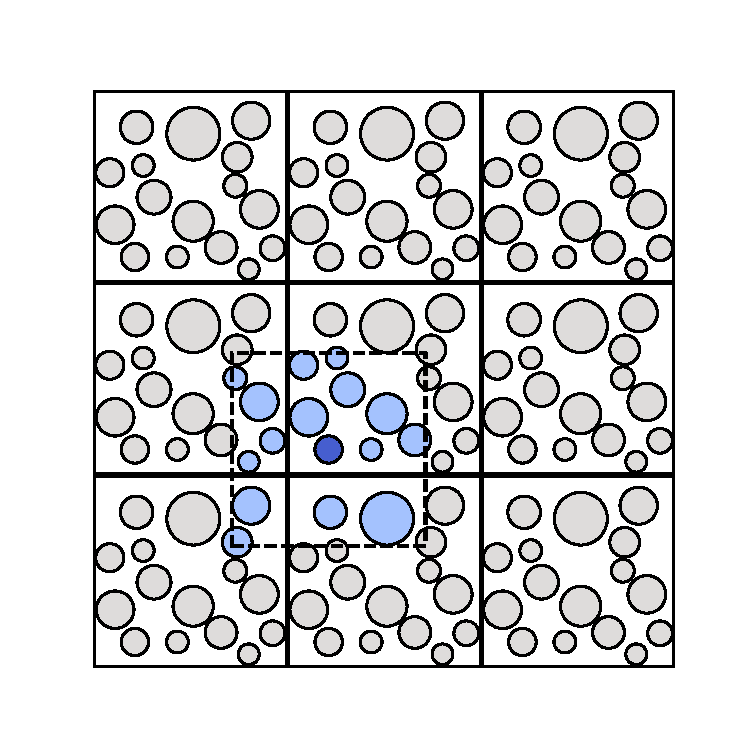
\includegraphics[width=5cm]{./figures/methods/mc_move_g.pdf}
	\caption{Simulation of bulk system is achieved using periodic boundary conditions, where a central cell is surrounded by repeated images of itself. A particle of interest (dark blue) then interacts with the nearest images of every other particle (light blue).}
	\label{fig:pbc}     
\end{figure}

Hard particle systems can be simulated using the Metropolis algorithm outlined in section \ref{ssec:metropolis}.
The system is initialised by selecting a random non\--overlapping configuration.
This can be achieved easily for low to medium densities by a greedy algorithm like random sequential addition, where particles are added successively in a manner which does not overlap with any previous particles \cite{Widom1966}.
For higher packing fractions a more sophisticated algorithm is needed \davidnote{Find refs}.

Once the initial configuration has been generated, it is evolved via two \mc{} moves.
The first is the displacement move, whereby a random particle is selected and translated according to a random vector with elements generated uniformly in the range $\left[-\delta,\delta\right]$.
If the displacement introduces any particle overlaps it is rejected, otherwise the system is updated to the new configuration, as illustrated in figure \ref{fig:hardmc1}\--\ref{fig:hardmc3}.
The value of $\delta$ is chosen for each simulation such that the proportion of accepted moves is $\sim 50\%$, allowing for efficient searching of configurational space.
The optimal value can be determined by continuous adjustment during equilibration.

The second is the swap move, where two random particles are selected their radii exchanged \cite{Grigera2001,Ninarello2017}. 
Once again a swap move is only accepted if it does not lead to any overlapping particles and is demonstrated in figure \ref{fig:hardmc4}\--\ref{fig:hardmc6}.
The swap move is used to increase the efficiency in simulations of polydisperse particles and is an example of how the design of \mc{} moves can be flexible and they do not have to have a direct physical basis. 
The swap move is attempted for every ten displacement moves. 

Finally, to remove the presence of an interface in the system, simulation is performed with periodic boundary conditions.
In this scheme the central simulation cell is repeated to form an infinite lattice, so that every particle experiences a bulk environment.
Coupled with this is the use of the minimum image convention, where each particle then only interacts with the nearest repeated image of all the remaining particles.
This is illustrated in figure \ref{fig:pbc}.
 
\subsection{Voronoi Construction}
\label{ssec:voronoi}


The hard particle configurations produced by \mc{} simulations are not in themselves network structures, rather simply a collection of correlated points.
The network structure is revealed by construction of a Voronoi diagram, which partitions the sample into a system of tessellating cells, where each cell encapsulates all the space closest to the associated particle \cite{Okabe1992}.
A \td{} Voronoi diagram is formed through the placement of dividing lines between the centroids of neighbouring particles. 
The intersection of these lines forms the characteristic tessellating polygons.

\begin{figure}[bt]
     \centering
     
     \begin{subfigure}[b]{0.22\textwidth}
         \centering
         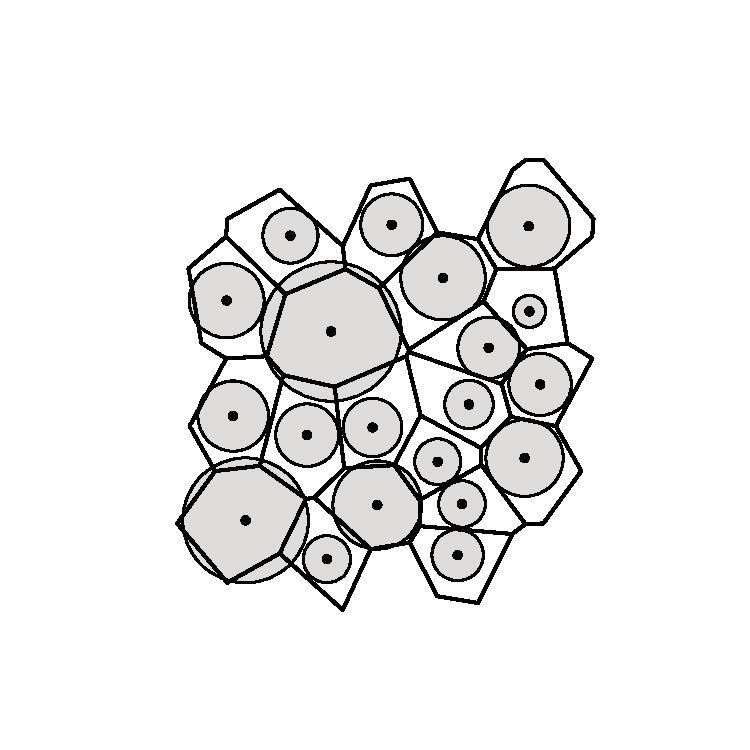
\includegraphics[width=\textwidth]{./figures/methods/voro_demo_vw.pdf}
         \caption{}
         \label{fig:vorodemov1}
     \end{subfigure}
     \hfill
     \begin{subfigure}[b]{0.22\textwidth}
         \centering
         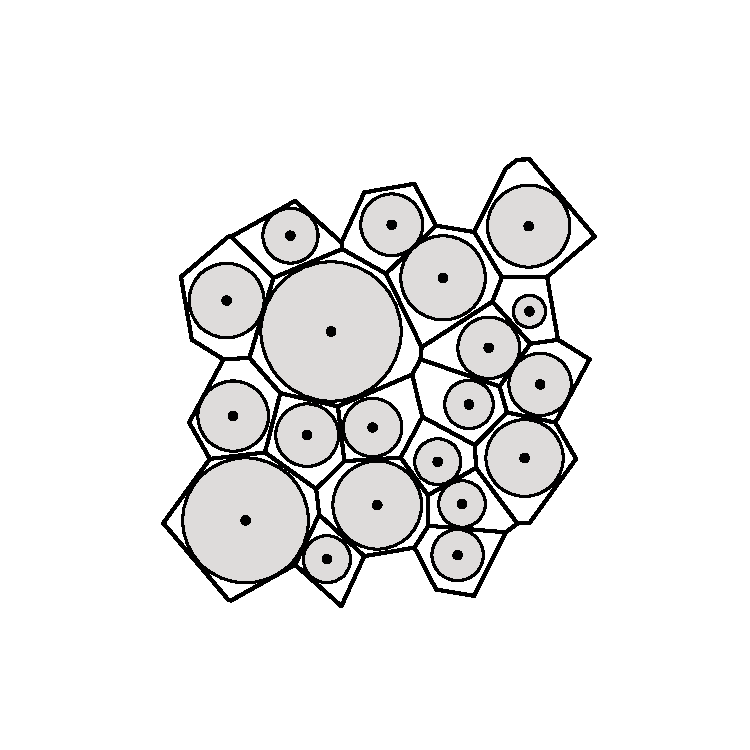
\includegraphics[width=\textwidth]{./figures/methods/voro_demo_rw.pdf}
         \caption{}
         \label{fig:vorodemor1}
     \end{subfigure}
     \hfill
     \begin{subfigure}[b]{0.22\textwidth}
         \centering
         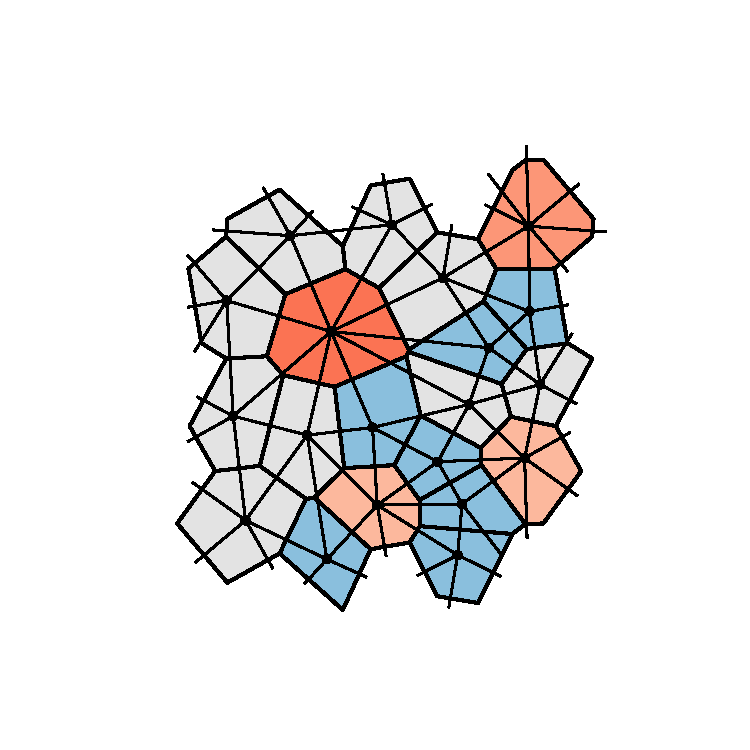
\includegraphics[width=\textwidth]{./figures/methods/voro_demo_vcd.pdf}
         \caption{}
         \label{fig:vorodemov2}
     \end{subfigure}
     \hfill
       \begin{subfigure}[b]{0.22\textwidth}
         \centering
         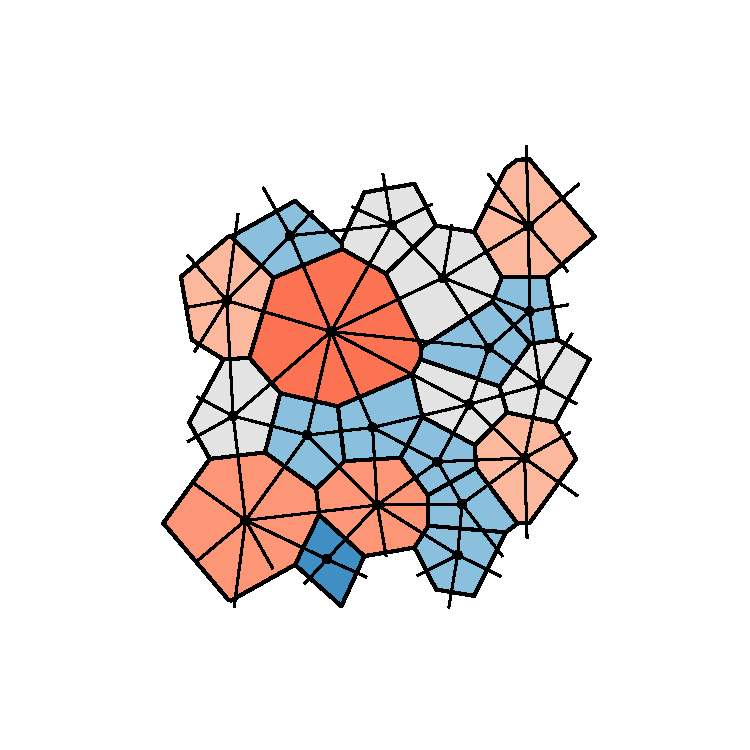
\includegraphics[width=\textwidth]{./figures/methods/voro_demo_rcd.pdf}
         \caption{}
         \label{fig:vorodemor2}
     \end{subfigure}
   
     \caption{Voronoi construction of a polydisperse hard disk system. Panels (a) and (b) compare the unweighted and weighted (radical) Voronoi tessellations respectively. The radical Voronoi assigns more volume to the larger particles to ensure a more equitable distribution of space, which can affect the underlying ring structure, shown in panels (c) and (d). The dual network, known as the Delaunay triangulation, is also overlaid.}
     \label{fig:vorodemo}
\end{figure}

In the simplest unweighted approach, the dividing line between two neighbouring particles separated by the Euclidean distance $r_{ij}$, is simply located midway between the particles at a distance $r_{ij} /2$. 
The elegance of the unweighted Voronoi diagram is that only the particle centroids are required for its construction, with no requirement for a cut-off parameter. 
Whilst the unweighted Voronoi tessellation is very effective for studying monodisperse particles, there are some limitations for polydisperse species. 
Specifically, the Voronoi partition underestimates the space assigned to large particles and overestimates that for small particles \-- a simple reflection of the lack of information on particle radii  (see figure \ref{fig:vorodemov1}). 
To rectify this, weighted modifications have been suggested which take account of the differences in radii \cite{Poupon2004}.

To construct a weighted Voronoi diagram, one simply adjusts the position of the dividing line, such that it is further from the particle with the greater weight. 
The weighting method used in this work is the so called radical tessellation introduced by Finney \cite{GELLATLY1982}. In this modification, the dividing line is placed a distance $d_i$ from particle $i$, given by:
\begin{equation}
	\label{eq:radical}
	d_i = \frac{w_i^2-w_j^2+r_{ij}^2}{2r_{ij}}\,,
\end{equation}
where $w_i$ and $w_j$ are the weights for each particle. 
The benefit of this method is that is adjusts the partitioning of space so that greater volume is assigned to the particles with larger weight, and is well designed so that all of the sample space remains accounted for - unlike some alternative constructions \cite{Richards1974}. 
In terms of the particle weights, the logical choice is simply the disk radii. 
This is because at the contact distance, $r_{ij} = R_i + R_j$, equation \eqref{eq:radical} shows that $d_i = R_i$ \ie{} the radical dividing line sits exactly between the two disks, producing the most equitable distribution of volume (see figure \ref{fig:vorodemor1}). 
Furthermore, when the radii are equal, $d_i = r_{ij} /2$ and the result from the standard unweighted Voronoi is regenerated as expected.
It is worth noting here that the weighting method can affect the ring sizes (\ie{} number of vertices) as well as the ring areas, as demonstrated in figures \ref{fig:vorodemov2},\ref{fig:vorodemor2}.

The outcome of the Voronoi construction is a system of percolating rings not dissimilar to those seen in materials.
The dual network, known as the Delaunay triangulation, is also obtained, which defines the nearest neighbours for each particle.
The main difference with atomic materials is that the polygon edge lengths and angles are not constrained by a potential model the ring structure is therefore completely entropically controlled.
The degree of disorder is then determined by the packing fraction, $\phi$, where decreasing the packing fraction leads to increased diversity in the ring statistics, as illustrated in figure \ref{fig:voromono}.
As can be seen there are some defects which are analogous to those seen in materials, such as the Stone\--Wales defect in figure \ref{fig:voromono2}, but others are not, as in figure \ref{fig:voromono1} which arise from very small perturbations in the crystalline lattice.
The limiting value as $\phi\rightarrow 0$ is well studied as the Poisson Voronoi diagram \cite{Boots1983,Tanemura2003}.
This corresponds to the Voronoi diagram formed from a random uniform array of points.
In this way Voronoi systems provide a good complement to compare and contrast with materials.

\begin{figure}[bt]
     \centering
          \begin{subfigure}[b]{0.24\textwidth}
         \centering
         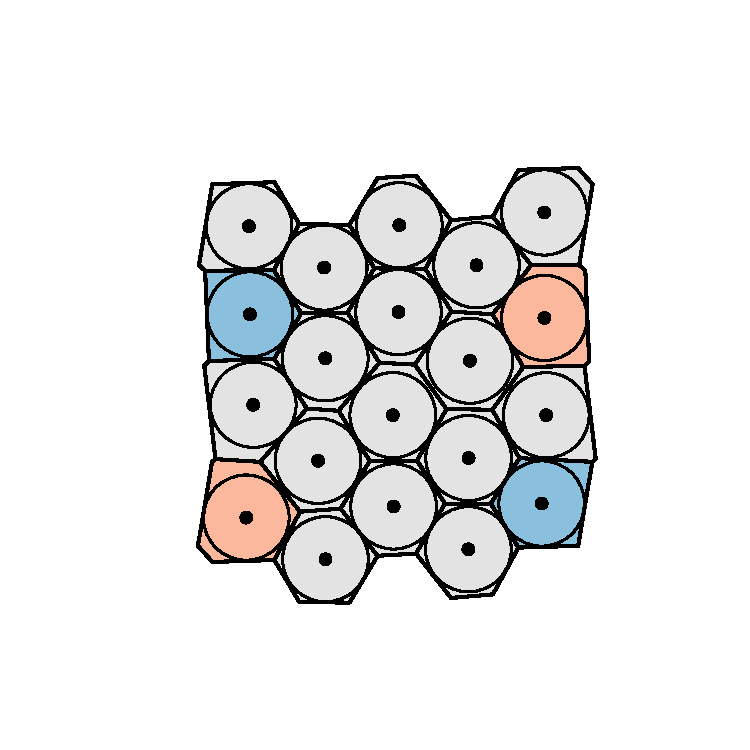
\includegraphics[height=3cm]{./figures/methods/voro_mono_80.pdf}
         \caption{$\phi=0.8$}
         \label{fig:voromono1}
     \end{subfigure}
     \hfill
     \begin{subfigure}[b]{0.24\textwidth}
         \centering
         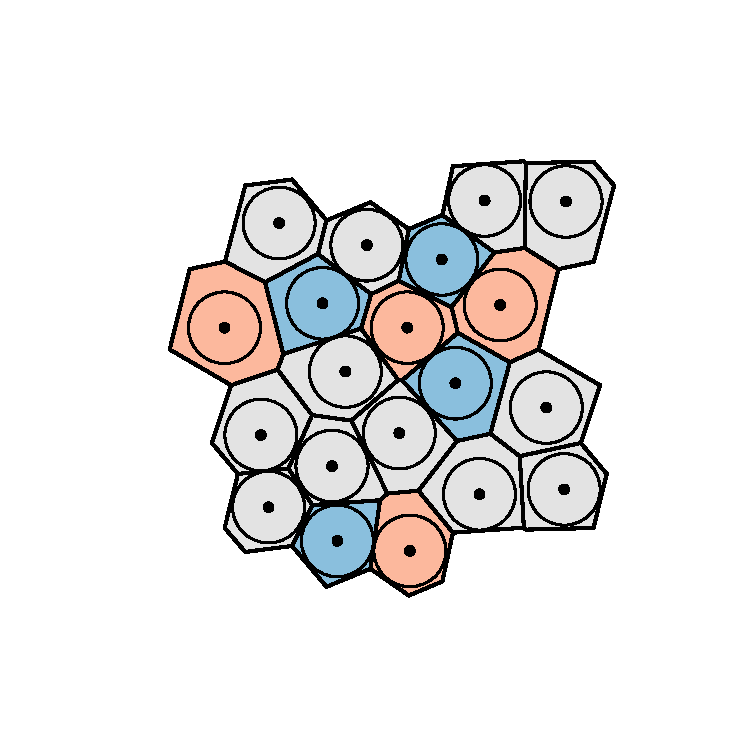
\includegraphics[height=3cm]{./figures/methods/voro_mono_60.pdf}
         \caption{$\phi=0.6$}
         \label{fig:voromono2}
     \end{subfigure}
     \hfill
     \begin{subfigure}[b]{0.24\textwidth}
         \centering
         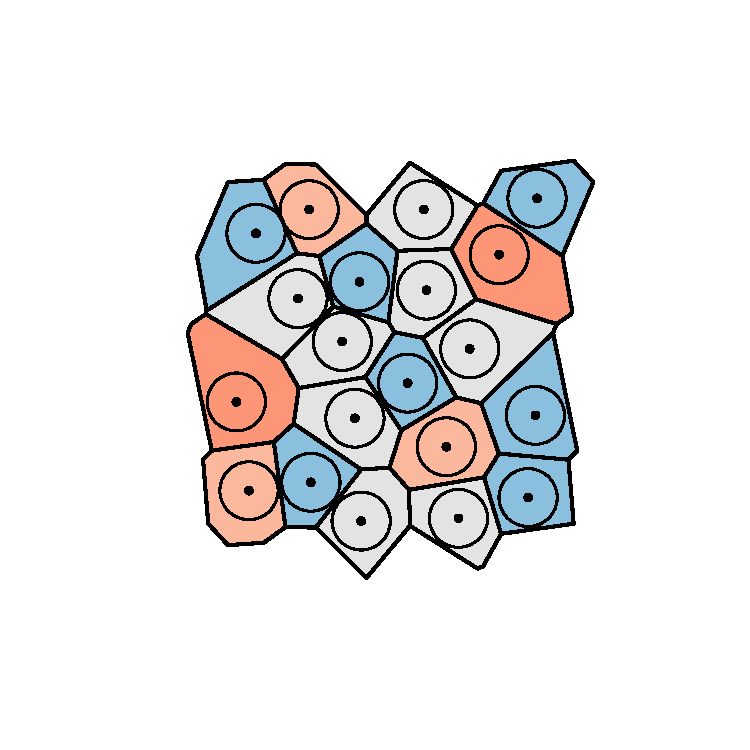
\includegraphics[height=3cm]{./figures/methods/voro_mono_40.pdf}
         \caption{$\phi=0.4$}
         \label{fig:voromono3}
     \end{subfigure}
     \hfill
       \begin{subfigure}[b]{0.24\textwidth}
         \centering
         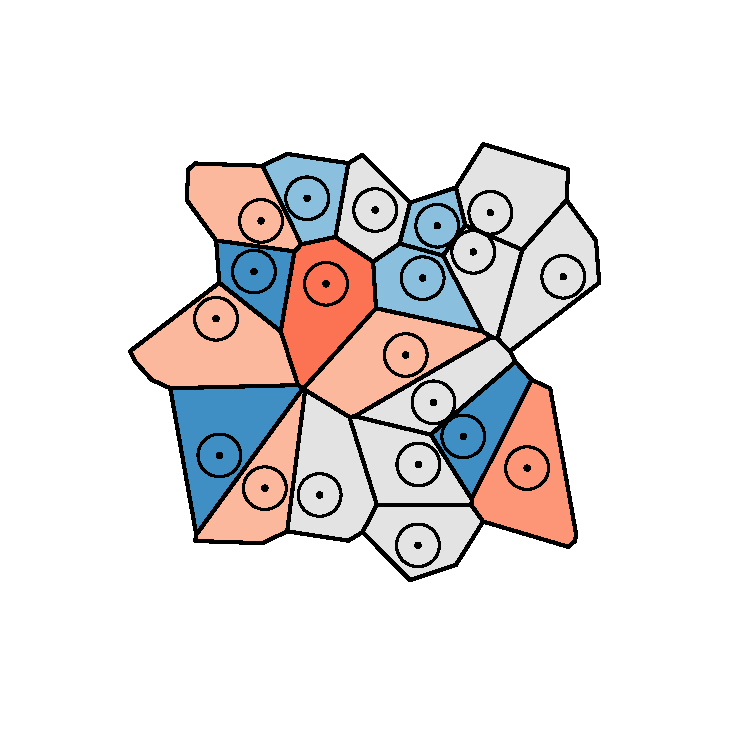
\includegraphics[height=3cm]{./figures/methods/voro_mono_20.pdf}
         \caption{$\phi=0.2$}
         \label{fig:voromono4}
     \end{subfigure}
     \caption{The ring structure in Voronoi diagrams is controlled through the packing fraction, $\phi$, of the underlying hard particle system. Ring diversity increases as packing fraction is lowered from $0.8\rightarrow 0.2$ in (a)\--(d).}
     \label{fig:voromono}
\end{figure}

\section{Analysis Methods}

\subsection{Bond Length and Angle Distributions}

\subsection{Radial Distribution Functions}







\chapter[Modelling Bilayer Materials]{Modelling Bilayer Materials}
\label{ch:bilayers}

\begin{chapterabstract}
A computationally tractable \mc{} method using triangle rafts is developed to generate bilayers of \sioii{} and related materials.
The method allows defect free networks of any given shape to be grown with both tuneable ring statistics and topologies, controlled by a combination of the ``allowed'' rings and the effective growth ``temperature''. 
Configurations are generated with \aw{} parameters commensurate with those obtained from an analysis of experimental configurations, improving significantly on previous methods.
The ability to efficiently grow configurations allows exploration of the structural basis of \lm’s law, where the commonly observed value of $p_6\approx0.4$ is presented as a balance between entropic and enthalpic factors. 
The deviations of ring areas from the ideal values are discussed and the relative insensitivity of the ring area to relatively strong distortions is highlighted.
\end{chapterabstract}

\section{Bilayer Materials}

An important class of \td{} materials which have emerged in the 21\st{} century are bilayers of silica, \sioii, and related species \cite{Buchner2017}.
These can be prepared experimentally by chemical vapour deposition on metal and graphene supports \cite{Huang2012,Lichtenstein2012a}.
As in the three\--dimensional glass, the basic building blocks of silica bilayers are vertex sharing \sioiv{} tetrahedra, maintaining full coordination for all atoms in the bulk \cite{Wilson2013}.
These are arranged such that three of the vertices are connected to tetrahedra in the same layer, with the final vertex being shared between layers acting as a ``bridge'' (figure \ref{fig:bilayer1}).
A consequence of these bridging oxygen atoms is to enforce a symmetry plane between the upper and lower layers.

Topologically, the symmetry plane means that these materials can be viewed as effective \td{} networks.
Taking one of the layers, without the bridging oxygens, and projecting the atoms onto the horizontal plane reveals a representation of vertex sharing triangles, referred to as a triangle raft (figure \ref{fig:bilayer2}).
The ring structure then emerges from the three\--coordinate network formed by connecting the silicon atoms of adjacent triangles as in figure \ref{fig:bilayer3}.
Indeed, scanning tunnelling microscopy (STM) has been used to directly visualise the ring structure in silica bilayers, revealing both crystalline and glassy arrangements and even the interface between the two   \cite{Loffler2010,Lichtenstein2012b}.

More recently experimentalists have also succeeded in synthesising bilayers of germania, \geoii{} \cite{Lewandowski2018,Lewandowski2019}.
\davidnote{Add a bit more experimental context here, discuss with Mark}
%These have the same fundamental structure as \sioii{}, but with more distorted tetrahedra \davidnote{Why again...some inorganic stuff...}.
%This can lead to a build up of strain and rumpling of the tetrahedral layers.
%\marknote{Have you discussed somewhere why they are doing this? Control of the pore size and pote
%density critical for gas separation applications....}
%\marknote{Note somewhere that making the GeO2 analogue is more difficult experimentally.....}

\begin{figure}[bt]
     \centering
     
     \begin{subfigure}[b]{0.3\textwidth}
         \centering
         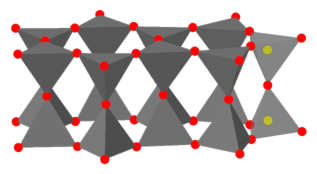
\includegraphics[width=\textwidth]{./figures/bilayers/mx2_bilayer_1.pdf}
         \vspace{-1mm}
         \caption{Tetrahedral bilayer}
         \label{fig:bilayer1}
     \end{subfigure}
     \hfill
	\begin{subfigure}[b]{0.3\textwidth}
         \centering
         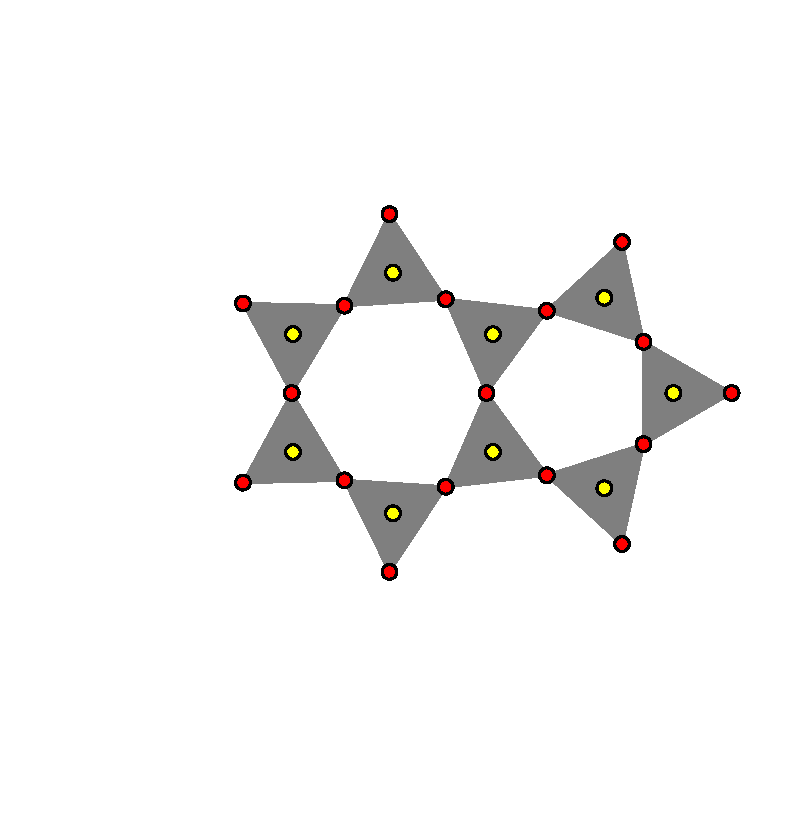
\includegraphics[width=\textwidth]{./figures/bilayers/mx2_bilayer_2.pdf}
         \caption{Triangle raft}
         \label{fig:bilayer2}
     \end{subfigure}
     \hfill
     \begin{subfigure}[b]{0.3\textwidth}
         \centering
         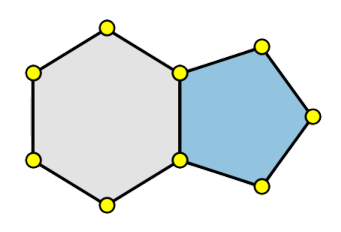
\includegraphics[width=0.8\textwidth]{./figures/bilayers/mx2_bilayer_3.pdf}
         \vspace{5mm}
         \caption{Ring structure}
         \label{fig:bilayer3}
     \end{subfigure}
     \hfill
     
     \caption{Silica bilayers of vertex sharing tetrahedra in (a) can be represented as a \td{} triangle raft in (b). Silicon and oxygen atoms are coloured yellow and red respectively. The ring structure then emerges from the three\--coordinate network comprising the silicon atoms, (c).}
     \label{fig:bilayer}
\end{figure}

\section{Review of Existing Methods}
\label{s:triraftexisting}

As mentioned in the  introduction, both \abinitio{} methods and classical molecular dynamics have been used in computational studies of silica bilayers, which often require a starting atomistic configuration  \cite{Bjorkman2013,Malashevich2016,Wilson2013,Roy2018}.  
One approach is to simply take an experimental sample as the starting structure. 
Whilst this may be on the surface the best solution, the experimental configurations may contain defects or areas where the image is corrupted \ie{} the configuration may not be ``pristine''.
Additionally, the location of each atom has an associated uncertainty which leads to discrepancies in the observed bond lengths and angles, which can be compounded by any out\--of\--plane distortions.
Whilst computational refinement can attenuate these problems \cite{Sadjadi2017,Wilson2018}, there remains the more fundamental question of how ``typical'' the available images are from experiment, as STM provides exceptional information but only on relatively small sample sizes.
Computational techniques can therefore prove a valuable tool for generating a large number of high\--quality configurations and corroborating experimental information.  

One current approach is to transform amorphous graphene configurations \cite{Wilson2013}.
Here amorphous samples of carbon are generated using a bond switching method (as outlined in section \ref{s:bondswitch}), before the carbon atoms are swapped from silicon and decorated with oxygens.
Whilst this is a valid approach, the method assumes that the two materials are topologically equivalent.
This is likely an oversimplification, as the presence of the bridging oxygens in silica afford the structure increased flexibility when compared to the carbon analogue.
This likely explains why this method has struggled to mirror experimentally observed values of the ring statistics and \aw{} parameter, with small and large ring proportions being under\--estimated \cite{Kumar2014}.

An alternative approach is to use molecular dynamics coupled with an effective pair potential to obtain viable configurations \cite{Roy2018}.
Such methods are relatively common, having been employed previously to study amorphous graphene \cite{Kumar2012}. 
Such methods offer the potential for generating realistic configurations but are difficult to control as the cooling rates which must be applied are necessarily huge compared to experimental rates. 
A potential artefact of the high cooling rates is the effectively freezing in of defect states, either in terms of local coordination environments or highly\--strained (three-membered) rings.
In addition, as with the method above, such methods appears to systematically underestimate the \aw{} parameter, indicative of too little structural ordering.

\section{Triangle Raft Method}
\label{s:triangleraft}

The motivation of this work was to develop a construction algorithm to generate samples of silica bilayers which can capture the full \td{} network topology; both the ring distribution \textit{and} correlations. 
The model should be able to explore all phases from crystalline to amorphous yet computationally efficient enough to produce configurations suitable for further high throughput calculations. 
To achieve this a grow-from-seed Monte Carlo algorithm has been developed, where rings are individually added to build a triangle raft.
This approach takes inspiration from the first hand\--built models, which have been noted to bear close resemblance to experimental structures \cite{Shackelford1982a,Buchner2016a}.
Such models were superseded by computational techniques designed to generate periodic configurations. 
However, the recent development in techniques to simulate aperiodic samples, such as sliding boundary conditions for molecular dynamics \cite{Theran2015}, makes this constraint no longer essential, and benefit may be gained from the added freedom of an aperiodic model.


\subsection{Potential Model}

As explained in figure \ref{fig:bilayer} it is possible to capture the full topology of silica bilayers with a simplified representation consisting of a network of vertex\--sharing \sioiii{} triangles. 
As the focus of this chapter is on generating a large number of samples with varying ring statistics, %to be used as a base for further calculations, 
working with this reduced representation is sufficient, as it provides a computationally efficient way to produce networks with the required \textit{topology}. 
The precise \textit{geometry} of the bilayer can be refined with advanced optimisation techniques if required \cite{Tangney2002}. 

In order to simulate bilayer systems in two dimensions, a suitable potential model is needed which captures the essential physics of the system: the local triangular environment of the \sioiii{} units and the relative energies of rings of different sizes. 
The model used here is modified from a relatively simple potential used in all\--atom bilayer calculations \cite{Wilson2013,Wilson2018}, a schematic for which is given in figure \ref{fig:trpotmodel}.
Each \sioiii{} unit has a harmonic potential acting between all three Si\---O pairs, and the three nearest\--neighbour O\---O pairs, given by:
\begin{equation}
	\label{eq:harmonic}
	\mathcal{U}_{ij} = \frac{\fk}{2}\left(r_{ij}-r_{ij}^{0}\right)^{2},
\end{equation}
where $\fk$ is a constant, $r_{ij}$ is the interatomic separation and $r_{ij}^{0}$ the equilibrium interatomic separation between $i,j$. 
The spring constant, $\fk$, is set to be very stiff, whilst the equilibrium separations are set according to elemental species such that $r_{\text{OO}}^{0}=\sqrt{3}\,r_{\text{SiO}}^{0}$, maintaining a set of ideal \sioiii{} triangles. 

The Si\---O\---Si angle, which determines the strain associated with different ring sizes, is controlled by a shifted and cut 24\--12 potential of the form:
\begin{equation}
	\mathcal{U}_{ij} = 
	\begin{cases}
	\epsilon \left[ \left(\frac{r_{0}}{r_{ij}}\right)^{24}-2\left(\frac{r_{0}}{r_{ij}}\right)^{12} \right] + \epsilon & r_{ij}\leq r_{0} \\
	0 & \text{otherwise}
	\end{cases}
\end{equation}
where $\epsilon$ is a constant and $r_{ij}$ is now the Si\---Si separation between atoms in adjacent triangles. 
It is the value of $r_{0}$ which sets the Si\---O\---Si angle at which strain begins to be felt and therefore the relative ring energies.
Taking the hexagonal lattice as being the zero in energy it follows that $r_{0}=2r_{\text{SiO}}$.
Rings which deviates increasingly from the ideal hexagon will therefore incur an increasingly energetic penalty.

\begin{figure}[bt]
     \centering
  
         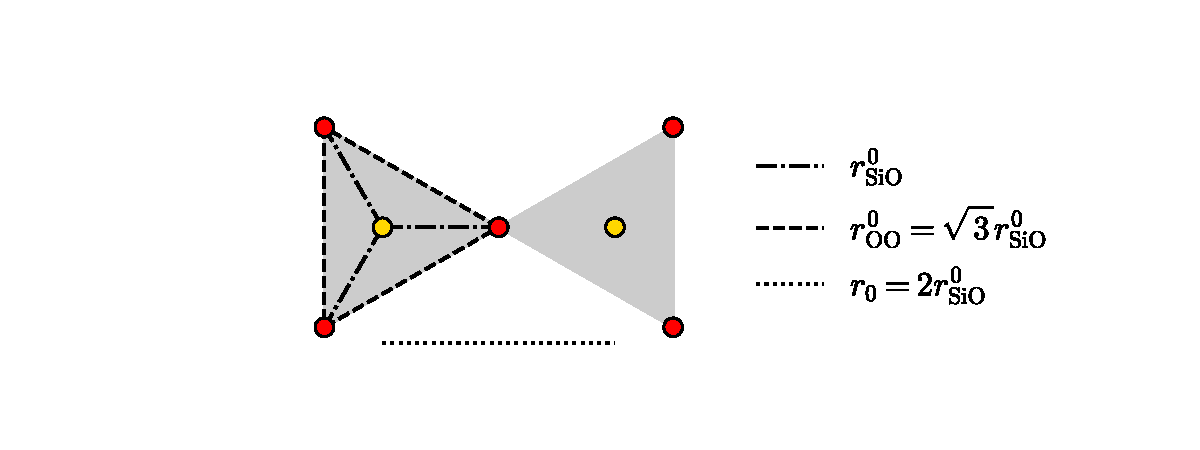
\includegraphics[width=0.6\textwidth]{./figures/bilayers/tr_pot_model.pdf}
 
     \caption{Schematic of the potential model in triangle rafts. Stiff harmonic springs (dashed and dashed\--dotted lines) preserve the triangular subunits, whilst the shifted and cut 24\--12 potential (dotted line) maintains an equilibrium angle of $120^\circ$ between neighbouring subunits.}
     \label{fig:trpotmodel}
\end{figure}

To summarise, the primary aim here is to generate topologies suitable for later investigation using more detailed (and hence more accurate but more
computationally-demanding) potential models. 
As a result, the harmonic springs simply control the local (triangular) geometries whilst the 24-12 potential controls the repulsion between these local polyhedra. 
These functions are chosen as deliberately simple to improve computational efficiency and achieve high throughput of idealised networks. 
Furthermore, the parameters $\fk$ and $\epsilon$ need have no direct physical meaning, simply controlling the
meaning of the system ``temperature'' as discussed below. 
The only requirement is that they generate energies of the same magnitude to allow for efficient
structural evolution.


\subsection{Algorithmic Details}


Using the model detailed above, a Monte Carlo construction algorithm has been developed which allows two\--dimensional networks to be built ring by ring in the shape of a specified function. The main steps of the algorithm are outlined below:
\begin{enumerate}
	\item Take a starting seed, such as a single ring or experimental configuration
	\item Select triangles on which to build the next ring (see figure \ref{fig:triraftalgsearch})
		\label{en:loopstart}
		\begin{enumerate}
			\item Overlay a function on the network (\eg{} circle, square)
			\item Check for atoms with dangling bonds lying inside the function region
			\item If no such atoms exist, systematically increase the function size until an atom is found
			\item Find the next nearest atoms which also have a dangling bonds
			\item Choose the two triangles that correspond to the largest starting ring size	
		\end{enumerate}
	\item Determine the probability of constructing rings of different sizes
		\begin{enumerate}
			\item Build trial rings in the range $k_{\text{min}}$ to $k_{\text{max}}$ (see figure \ref{fig:triraftalgtrial})
			\item Geometry optimise the local structure and calculate minimised potential energy (as explained in section \ref{s:geomopt})
			\item Calculate the probabilities of each ring occurring, $P_k$, equation \eqref{eq:probdist}
		\end{enumerate}
	\item Accept single trial ring according to the probability distribution
		\label{en:loopend}
	\item Repeat steps \ref{en:loopstart} $\rightarrow$ \ref{en:loopend} until the target number of rings is reached
\end{enumerate}
The probability of a ring of size $k$ being accepted, $P_k$, is given by the equation:
\begin{equation}
	\label{eq:probdist}
	P_k=\frac{ \exp{\left[-\left(\mathcal{U}_{k}-\mathcal{U}_k\right)/T\right]}}{\sum\limits_{k}\exp{\left[-\left(\mathcal{U}_{k}-\mathcal{U}_{0}\right)/T\right]}},
\end{equation}
where $\mathcal{U}_k$ and $\mathcal{U}_{0}$ correspond to the energy of the trial structure and lowest energy of all trial structures respectively, and $T$ is a ``temperature''. 
The parameter $T$ controls how easily the potential energy landscape can be explored, and therefore how accessible strained rings become. 
In the low $T$ limit, the acceptance probabilities are dominated by the energy term, and the rings which are selected will be those with the lowest energy. 
Note that this is not necessarily the 6-ring, but rather is dependent on the local environment. On the other hand, in the high $T$ limit, the acceptance probabilities are approximately equal, and rings are selected on a more random basis. 
This is demonstrated in table \ref{tab:prob}, using the example configurations from figure \ref{fig:triraftalgtrial}. 
The ``temperature'' parameter is therefore the primary method for controlling the distribution of ring sizes in constructed networks.

\begin{figure}[bt]
     \centering
     
     \begin{subfigure}[b]{0.45\textwidth}
         \centering
         \includegraphics[width=2.5cm]{./figures/bilayers/alg_search_1.pdf}
         \vspace{-1mm}
         \caption{}
         \label{fig:triraftalgsearch1}
     \end{subfigure}
     \hfill
	\begin{subfigure}[b]{0.45\textwidth}
         \centering
         \includegraphics[width=2.5cm]{./figures/bilayers/alg_search_2.pdf}
         \caption{}
         \label{fig:triraftalgsearch2}
     \end{subfigure}
     \hfill
     \caption{Panel (a) shows how triangles used to construct a ring are initially selected. There are no atoms with dangling bonds within the first search region (blue dashed line), and so the search area is extended (red dashed line), where triangles A and B are found. Panel (b) gives the three possibilities for the triangles that will form part of the constructed ring: A–C–D–B, A–E, B–F. As A–C–D–B corresponds to the largest starting ring size this is selected.}
     \label{fig:triraftalgsearch}
     
     \begin{subfigure}[b]{0.18\textwidth}
         \centering
         \includegraphics[width=\textwidth]{./figures/bilayers/alg_4.pdf}
         \caption{}
         \label{fig:triraftalgtrial1}
     \end{subfigure}
     \hfill
     \begin{subfigure}[b]{0.18\textwidth}
         \centering
         \includegraphics[width=\textwidth]{./figures/bilayers/alg_5.pdf}
         \caption{}
         \label{fig:triraftalgtrial2}
     \end{subfigure}
     \hfill
     \begin{subfigure}[b]{0.18\textwidth}
         \centering
         \includegraphics[width=\textwidth]{./figures/bilayers/alg_6.pdf}
         \caption{}
         \label{fig:triraftalgtrial3}
     \end{subfigure}
     \hfill
      \begin{subfigure}[b]{0.18\textwidth}
         \centering
         \includegraphics[width=\textwidth]{./figures/bilayers/alg_7.pdf}
         \caption{}
         \label{fig:triraftalgtrial4}
     \end{subfigure}
     \hfill
      \begin{subfigure}[b]{0.18\textwidth}
         \centering
         \includegraphics[width=\textwidth]{./figures/bilayers/alg_8.pdf}
         \caption{}
         \label{fig:triraftalgtrial5}
     \end{subfigure}
     \hfill
     \caption{Geometry optimised structures for trial rings in the range $k = 4-8$. The ring structure is shown along with the \sioiii{} triangle}
     \label{fig:triraftalgtrial}
    
\end{figure}

\begin{table}[bt]
	\centering
	\caption{Variation of acceptance probabilities with temperature for the configurations in figure \ref{fig:triraftalgtrial}.}
	\label{tab:prob}
	\begin{tabular}{c c c c c c}
	\toprule
	$P_{k}$ & 4 & 5 & 6 & 7 & 8 \\[0.5mm]
	\midrule
	$T=10^{-4}$ & 0.0000 & 1.0000 & 0.0000 & 0.0000 & 0.0000 \\[0.5mm]
	$T=10^{-3}$ & 0.0000 & 0.8837 & 0.1162 & 0.0001 & 0.0000 \\[0.5mm]
	$T=10^{-2}$ & 0.0336& 0.4104 & 0.3351 & 0.1659 & 0.0550 \\[0.5mm]
	$T=10^{-1}$ & 0.1734 & 0.2227 & 0.2183 & 0.2034 & 0.1822 \\[0.5mm]
	$T=10^{0}\;\;$ & 0.1973 & 0.2023 & 0.2018 & 0.2004 & 0.1982 \\[0.5mm] 
	\bottomrule	
	\end{tabular}
\end{table}

\section{Properties of Triangle Rafts}

The triangle raft method is evaluated in terms of its effectiveness in producing configurations which accurately replicate the network properties of experimental silica bilayers \ie{} the ring statistics and \aw{} parameter.
It is also compared against the existing methods introduced in section \ref{s:triraftexisting}, namely generation from amorphous graphene or molecular dynamics.
This is performed in the wider context of systematically varying the model parameters to explore the behaviour of generic networks of this type.

\subsection{Network Growth}
 
The triangle raft method is robust and controllable, and is able to generate configurations with tuneable ring statistics and topologies.
Results will largely focus on the system where $k=4-10$, denoted $\br{4}{10}$, mimicking the experimentally observed range for silica bilayers. 
Six example configurations are given in figure \ref{fig:triraft}, which are generated with a range of temperatures and growth geometries. 
Figures \ref{fig:triraft1}\--\ref{fig:triraft4} provide a good qualitative analysis of the effect of temperature on the ring structure. 
At low temperature a phase boundary can be seen separating crystalline and amorphous regions, as seen in experimental silica bilayers \cite{Lichtenstein2012b}. 
In these samples although the proportion of small and large rings is low, their positions are highly correlated and chain structures of alternating rings sizes are clearly present. 
These motifs are reminiscent of defects found in a wide range of materials, including amorphous graphene and thin silicon and germanium oxides \cite{Bjorkman2013,Robertson2012,Buchner2017,Lewandowski2018}. 
The increase in temperature is coupled with the emergence of rings of more extreme sizes and regions which could be viewed as nano\--crystalline are dispersed. 
The high temperature limit reveals a fully amorphous structure.

\begin{figure}[h!]
     \centering
     
     \begin{subfigure}[b]{0.35\textwidth}
         \centering
         \includegraphics[width=\textwidth]{./figures/bilayers/mx2_sq_1.pdf}
         \caption{}
         \label{fig:triraft1}
     \end{subfigure}
     \hspace{1cm}
     \begin{subfigure}[b]{0.35\textwidth}
         \centering
         \includegraphics[width=\textwidth]{./figures/bilayers/mx2_sq_2.pdf}
         \caption{}
         \label{fig:triraft2}
     \end{subfigure}
     \hfill
     %\vspace{0.5cm}
     
     \begin{subfigure}[b]{0.35\textwidth}
         \centering
         \includegraphics[width=\textwidth]{./figures/bilayers/mx2_sq_3.pdf}
         \caption{}
         \label{fig:triraft3}
     \end{subfigure}
     \hspace{1cm}
      \begin{subfigure}[b]{0.35\textwidth}
         \centering
         \includegraphics[width=\textwidth]{./figures/bilayers/mx2_sq_4.pdf}
         \caption{}
         \label{fig:triraft4}
     \end{subfigure}
     \hfill
     %\vspace{0.5cm}
     
      \begin{subfigure}[b]{0.35\textwidth}
         \centering
         \includegraphics[width=\textwidth]{./figures/bilayers/mx2_circle.pdf}
         \caption{}
         \label{fig:triraft5}
     \end{subfigure}
     \hspace{1cm}
      \begin{subfigure}[b]{0.35\textwidth}
         \centering
         \includegraphics[width=\textwidth]{./figures/bilayers/mx2_heart.pdf}
		\hfill         
         
         \caption{}
         \label{fig:triraft6}
     \end{subfigure}
     
     \caption{Example $1,000$ ring configurations generated with different temperatures and shapes. Panels (a) through (d) show square lattices grown at $T=10^{-4.0},\,10^{-3.0},\,10^{-2.5},\, 10^{-2.0}$ respectively. The samples show the increasing diversity in ring structure as temperature is increased. Panels (e), (f) show configurations with alternative lattice shapes at $T=10^{-3.0}$, demonstrating the flexibility of the method in growing samples with variable geometries. Rings are coloured according to size with $k<6$ as blue, $k=6$ as grey and $k>6$ as red.}
     \label{fig:triraft}
\end{figure}

Figures \ref{fig:triraft5} and \ref{fig:triraft6} give examples of the diverse geometries in which samples may be constructed. 
It is interesting to note that even ``difficult'' shapes, such as those containing concave regions and cusps, do not prevent growth.  
Although the shape does not affect the network topology and is in a sense arbitrary, certain calculations may benefit from the different configurational shapes. 
For instance, molecular dynamics with sliding boundary conditions requires fitting of a smooth function to the sample perimeter, which is facilitated by having a near\--circular form.
Other areas such as percolation problems may benefit from square samples.

\subsection{Network Properties}
\label{s:triraftnetprop}

The quantitative relationship between temperature and ring structure was investigated for three systems of varying ring size ranges;  $\br{5}{7}$, $\br{4}{8}$ and $\br{4}{10}$. 
For each system, 100 samples consisting of 1000 rings were grown at temperatures between $T=10^{-4.5}\rightarrow 10^{-1.5}$. 
The evolution of the combined ring statistics with temperature is presented in figure \ref{fig:trpk}. 
Figures \ref{fig:trpk1}\--\ref{fig:trpk3} give bar representations of the ring size distributions for the three systems, which show different behaviours. 
For $\br{5}{7}$ the individual $p_k$ are all monotonically increasing ($k\neq 6$) or decreasing ($k=6$) functions, but both $\br{4}{8}$ and $\br{4}{10}$ have $p_k$ containing maxima. 
Additionally, both $\br{5}{7}$ and $\br{4}{8}$ achieve uniform distributions in the high temperature limit but $\br{4}{10}$ does not. 

This disparity in behaviour can largely be traced back to the constraint of Euler's theorem. 
As $\br{5}{7}$ comprises of just three ring sizes, Euler's formula demands that $p_5=p_7=\left(1-p_6\right)/2$ and so the system is relatively well defined. 
Hence, as the 5 and 7-rings are more strained than the 6-ring, $p_5$ and $p_7$ show a systematic increase with temperature. 
Furthermore, the uniform equilibrium distribution can only satisfy Euler's formula when the ring size range is symmetric about 6, as is observed for $\br{5}{7}$ and $\br{4}{8}$. 
The form of the ring statistics at intermediate temperatures and for $\br{4}{10}$ follow the maximum entropy solutions according to \lm's law, discussed in section \ref{s:lemaitre} and later in this section.

\begin{figure}[bt]
     \centering
     
     \begin{subfigure}[b]{0.45\textwidth}
         \centering
         \includegraphics[width=\textwidth]{./figures/bilayers/triraft_57.pdf}
         \caption{$\br{5}{7}$}
         \label{fig:trpk1}
     \end{subfigure}
     \hfill
	\begin{subfigure}[b]{0.45\textwidth}
         \centering
         \includegraphics[width=\textwidth]{./figures/bilayers/triraft_48.pdf}
         \caption{$\br{4}{8}$}
         \label{fig:trpk2}
     \end{subfigure}
     \hfill
     
	\vspace{0.5cm}          
     \begin{subfigure}[b]{0.45\textwidth}
         \centering
         \includegraphics[width=\textwidth]{./figures/bilayers/triraft_410.pdf}
         \caption{$\br{4}{10}$}
         \label{fig:trpk3}
     \end{subfigure}
     \hfill
	\begin{subfigure}[b]{0.45\textwidth}
         \centering
         \includegraphics[width=\textwidth]{./figures/bilayers/triraft_line_410.pdf}
         \caption{$\br{4}{10}$}
         \label{fig:trpk4}
     \end{subfigure}
     \hfill
   
     \caption{Variation in ring statistics with temperature over a given allowable $k$\--range. Panels (a)-(c) show bar graph representations of the ring statistics, coloured by temperature, for the $\br{5}{7}$, $\br{4}{8}$ and $\br{4}{10}$ systems, respectively. Panel (d) gives an alternative line graph representation of the ring statistics for $\br{4}{10}$, coloured by ring size, along with the Aboav\--Weaire parameter. The temperature which gives the best match to the experimentally observed amorphous region is also highlighted (vertical black dashed line).}
     \label{fig:trpk}
\end{figure}

The ring distribution for $\br{4}{10}$ is also shown as a function of temperature in figure \ref{fig:trpk4}, along with the value of the \aw{} parameter, $\alpha$, allowing for more facile comparison with experiment. 
The temperature which gives the best agreement between our model and amorphous experimental samples is highlighted by the vertical dashed line. 
The values of $p_k$ and $\alpha$ are provided in table \ref{tab:trpk}, alongside results from two experimental samples. 
It is evident that the model can be successfully tuned to match the topology of the experimental system. 
Not only are the ring distributions in very good accordance, but also the ring correlations, which have until now proved difficult to capture. 
This provides confidence that this simplified but physically motivated triangle raft model is able to reproduce the behaviour of real systems.

\begin{landscape}
\begin{table}
\centering
\caption{Comparison of silica bilayer samples from experiment, computational modelling and theory.}
\label{tab:trpk}
\begin{threeparttable}
\begin{tabular}{@{}ccccccccccc@{}}
\toprule
& \multicolumn{2}{c}{Experiment} & \phantom{xxx} & \multicolumn{4}{c}{Computation} & \phantom{xxx} & \multicolumn{1}{c}{Theory} \\ 
\cmidrule{2-3} \cmidrule{5-8} \cmidrule{10-10}
& Ru(0001) \cite{Buchner2016a} & Graphene \cite{Huang2012} & & MC\tnote{a}\, \cite{Kumar2014} & MC\tnote{a}\, \cite{Kumar2014} & MD\tnote{b}\, \cite{Roy2018} & TR\tnote{c} & & \lm{} \cite{Gervois1992}  \\ 
\midrule
$N$ & 317    & 444    &&    216 & 418      & $16 \times 85000$ & $1000 \times 100$ && \--- \\ 
$p_3$  &0.0000 & 0.0000 && 0.00 & 0.00     & 0.0038            & 0.0000 && 0.0000 \\ 
$p_4$  &0.0379 & 0.0383 && 0.02   & 0.00     & 0.0537            & 0.0295 && 0.0280 \\  
$p_5$  &0.2744 & 0.2725 && 0.33   & 0.37     & 0.2686            & 0.2786 && 0.2834 \\
$p_6$  &0.4448 & 0.4189 && 0.37   & 0.32     & 0.3773            & 0.4234 &&  0.4200 \\  
$p_7$  &0.1609 & 0.2117 && 0.21   & 0.25     & 0.2224            & 0.2034 && 0.2077 \\  
$p_8$  &0.0757 & 0.0495 && 0.07   & 0.06     & 0.0602            & 0.0544 && 0.0518 \\ 
$p_9$  &0.0063 & 0.0068 && <0.01  & 0.00     & 0.0118            & 0.0097 && 0.0082 \\
$p_{10}$  &0.0000 & 0.0023 && 0.00 & 0.00  & 0.0018            & 0.0010 && 0.0009 \\
$p_{>10}$  &0.0000 & 0.0000 && 0.00 & 0.00 & 0.0004            & 0.0000 && 0.0000 \\ 
$\mu_2$ &  0.9460 & 0.9333 &&  0.94 & 0.86 & 1.1302 & 0.9208 && 0.8985 \\ 
$\alpha$  &0.32   & 0.33 && 0.18 & 0.23 & 0.25 & 0.32 && \--- \\
\bottomrule
\end{tabular}
\begin{tablenotes}
  Note: Each method is given alongside the number of rings in the sample, $N$, followed by the ring statistics, $p_k$, the second moment of the ring statistics, $\mu_2$, and the \aw{} parameter, $\alpha$ \\
  \item[a] Bond switching \mc{} (graphene potential)
  \item[b] Molecular dynamics
  \item[c] Triangle rafts, this work, $T=10^{-3}$
\end{tablenotes}
\end{threeparttable}
\end{table}
\end{landscape}

Table \ref{tab:trpk} also lists the ring statistics obtained from previous computational studies which used both Monte Carlo and molecular dynamics methods. 
As mentioned in the review of these methods above, neither fully succeeds in accurately capturing the topology of silica bilayers.
Kumar \etal{} attempted to transform an amorphous graphene structure generated from bond switching \mc{} into a silica bilayer.
The ring statistics of the resulting structure were approximately correct, but the proportion of 5\-- and 6\-- rings over\-- and under\--estimated respectively.
In addition the \aw{} parameter was substantially lower than experiment, indicating a relative lack of structure in the ring ordering.
The origin of these discrepancies is likely the use of a graphene potential model.
The increased stiffness of the carbon network (which unlike silica lacks bridging oxygens) means a high temperature must be used to obtain an amorphous structure with the required disorder.
This leads to heavily distorted rings (as noted in the original paper) which reduces the requirement for small rings to be adjacent to large.

Roy \etal{} have an alternative approach of generating configurations with an effective pair potential and molecular dynamics.
As can be seen the ring statistics are closer to the experimental values, but now contain artefacts, with a significant fraction of highly strained 3\--membered rings and large rings up to $k=14$.
These manifest as a result of the artificially high cooling rates in the computational studies which trap defect states in the configurations. 
Once again the final \aw{} parameter, $\alpha$, is underestimated.

It is worth re\--emphasising here that the triangle raft method is able to replicate experimental values of both $p_k$ and $\alpha$, due to its tuneable approach and ``organic'' growth mechanism, where sample formation is not influenced by enforced periodicity. 
Beyond this, the controllable nature of the method also allows insight into key questions about silica bilayers, for instance the form of the ring distribution in this amorphous phase. 
As detailed in section \ref{s:lemaitre}, the maximum entropy ring distribution can be calculated numerically given the value of $p_6$.
For example, table \ref{tab:trpk} gives the maximum entropy solution for $p_6=0.42$, which agrees very well with the results from triangle rafts and experiment.
This second moment of the distribution, $\mu_2$, is then uniquely related to $p_6$ via \lm's law, shown as the black line in in figure \ref{fig:trlm1}.


\begin{figure}[bt]
     \centering
     
     \begin{subfigure}[b]{0.45\textwidth}
         \centering
         \includegraphics[width=\textwidth]{./figures/bilayers/tri_raft_lm_1.pdf}
         \caption{}
         \label{fig:trlm1}
     \end{subfigure}
     \hfill
     \begin{subfigure}[b]{0.45\textwidth}
         \centering
         \includegraphics[width=\textwidth]{./figures/bilayers/tri_raft_lm_3.pdf}
         \caption{}
         \label{fig:trlm2}
     \end{subfigure}
     \hfill
     \begin{subfigure}[b]{0.45\textwidth}
         \centering
         \includegraphics[width=\textwidth]{./figures/bilayers/tri_raft_lm_2.pdf}
         \caption{}
         \label{fig:trlm3}
     \end{subfigure}
     \hfill

     \caption{Evolution of ring statistics (a), entropy (b) and potential energy (c) of triangle rafts with temperature. The experimental value of $p_6\approx 0.4$ occurs just before the exponential increase in potential energy, reflecting the balance of energetic and entropic factors.}
     \label{fig:trlm}
\end{figure}


However, \lm's law gives no information on why a particular maximum entropy distribution is found for a given system.
The triangle raft method allows systematic generation of configurations with different $p_6$ values by tuning the temperature parameter. 
The resulting configurations follow \lm's law across the entire temperature range. 
Figures \ref{fig:trlm} gives the results from the individual 1000 ring samples, coloured by temperature.
Figures \ref{fig:trlm1} and \ref{fig:trlm2} compare the observed $\mu_2$ and $\mathcal{S}$ (entropy) of the generated configurations to those expected from \lm's law, showing the law provides a good fit, with only a small deviation observed for $p_k>0.5$. 

Figure \ref{fig:trlm3} plots the geometry optimised potential energy of the samples against $p_6$, which increases as the ring sizes become more diverse. 
The curve is split into two regimes, with gradual increase in energy from $p_6=1.0\rightarrow 0.4$ followed by exponential increase for $p_6<0.4$. 
This is consistent with the information in figure \ref{fig:trpk4} which shows that below $p_6\approx 0.4$, not only does the number of extreme ring sizes increase rapidly, but they become less correlated with a lower $\alpha$, decreasing the number of favourable small\--large ring pairings.

It can now be proposed why the experimental amorphous distributions are found with a value of $p_6\approx 0.4$. 
The system aims to maximise entropy by obtaining a ring distribution along the \lm{} curve with the minimum $p_6$ possible. 
However, for $p_6<0.4$ the energetic cost becomes prohibitively large, as higher entropy distributions can only be achieved by increasing the proportion of extreme ring sizes at the expense of relatively low strain 5- and 7- rings.
Interestingly it is also evident why no configurations are present below $p_6\approx 0.16$, even at the highest temperature.
Below this point, the entropy of the $\br{4}{10}$ system decreases whilst the energy continues to rise and so there is no driving force to sample this area of phase space.

\subsection{Physical Properties}
\label{s:trphysprop}

As an additional check that the developed triangle raft model behaves physically, 
the angle distribution between adjacent \sioiii{} units, $f\left(\theta\right)$, was calculated for the $\br{4}{10}$ system across the range of temperatures studied. 
The results are summarised in figure \ref{fig:trang}. 
The angle distributions are necessarily symmetric about $120^\circ$, as each triangle pair contributes two complementary angles. 
At lower temperatures the distribution is dominated by angles close to $120^\circ$, as a consequence of the large proportion of near strainless six membered rings.
Furthermore, at the temperature corresponding to the amorphous experimental region, $T=10^{-3}$, the distribution has a similar extent to the angle distribution found in experimental samples (see for example figure 7 reference \cite{Roy2018}). 
However, as the temperature increases, the form of $f\left(\theta\right)$ does not simply broaden as might be expected, but becomes bimodal. 
This can be rationalised by considering the angles that would be present in regular polygons of different sizes, marked by vertical lines in figure \ref{fig:trang}.  These ideal angles are clustered away from the mean value of $120^\circ$, and hence increasing the diversity of ring sizes through temperature acts to shift the most commonly observed angles from the central value of $120^\circ$. 
It is therefore interesting to note that increasing structure in the angle distribution does not necessarily translate to increased order in the atomic configurations.

\begin{figure}[bt]
     \centering
     
     \begin{subfigure}[b]{0.45\textwidth}
         \centering
         \includegraphics[width=\textwidth]{./figures/bilayers/tri_raft_angle.pdf}
         \caption{}
         \label{fig:trang}
     \end{subfigure}
     \hfill
     
     \begin{subfigure}[b]{0.45\textwidth}
         \centering
         \includegraphics[width=\textwidth]{./figures/bilayers/tri_raft_area.pdf}
         \caption{}
         \label{fig:trarea}
     \end{subfigure}
     \hfill
     \begin{subfigure}[b]{0.45\textwidth}
         \centering
         \includegraphics[width=\textwidth]{./figures/bilayers/ellipse_area.pdf}
         \caption{}
         \label{fig:trellipse}
     \end{subfigure}
     \hfill

     \caption{Panel (a) gives the ring angle distribution function for triangle rafts formed at different temperatures. Panel (b) compares the regularity of rings in computational and experimental amorphous configurations, with points indicating the mean value and bars corresponding to the standard deviation. Experimental data is taken from ref. \cite{Kumar2014}. Panel (c) shows the effect on the area when distorting a circle to an ellipse whilst maintaining a constant perimeter length.}
     \label{fig:trangarea}
\end{figure}

A final check comes from examining the ring areas in the generated configurations.
Inspection of amorphous experimental samples reveals that the rings appear highly regular in shape. 
This can be quantified by determining the average dimensionless area for each ring size, $A_k$, and comparing it to the area of the corresponding regular polygon, $A_k^0$, where:
\begin{align}
	A_k &= \frac{\langle Area\left(k\right) \rangle}{\left(r_{\text{SiSi}}^{0}\right)^2}, \label{eq:trarea} \\[0.5em]
	A_k^0 &= \frac{k}{4\tan\left(\pi / k \right)} \label{eq:trarea0}.
\end{align}
As the regular polygon has the maximum achievable area for a given ring size, the ratio $A_k / A_k^0$ is expected to lie in the range $0\rightarrow 1$, with a lower value corresponding to increased deviation from regularity, and assuming $r_{\text{SiSi}}^{0}$ to be fixed.

The study by Kumar \etal{} found that whereas for experimental configurations, $A_k / A_k^0 \approx 1$, configurations generated using thier bond switching method generally displayed ratios much less than unity \cite{Kumar2012}, indicative of large distortions in the ring structure. 
For larger rings, a value of $A_k / A_k^0 > 1$ was also found, which can only be achieved if there is appreciable bond stretching (see equations \eqref{eq:trarea}, \eqref{eq:trarea0}). 

The analogous results for the method presented in this chapter can be found in figure \ref{fig:trarea}, for $T=10^{-3}$. 
This figure demonstrates that there is now good agreement between experimental and computational results. 
In both cases the deviation from regularity increases with ring size, as the flexibility of the rings increases. 
Again it can be proposed that the difference between current and previous methods could be due to the lack of enforced periodicity on the system. 
By allowing the network to grow relatively freely, the system can avoid a build up of strain associated with maintaining periodic boundaries.

Even with this analysis, an argument can be made that by visual inspection the rings in the experimental configurations are still more regular than those generated from computational samples. 
Therefore one can consider if deformation of a ring should be expected to lead to significant reduction in area. 
This can be explored by considering the distortion of a circle to an ellipse. 
The degree of distortion can be described by the eccentricity of the ellipse,
\begin{equation}
	\xi = \left(1-\frac{b^2}{a^2}\right)^{1/2},
\end{equation}
where $a$, $b$ are the major and minor axis radii respectively. 
This change in area with distortion is shown in figure \ref{fig:trellipse}, the calculation of which can be found in appendix \ref{app:derivellipse}. 
As can be seen, a large degree of eccentricity is needed for a significant change in the observable area. 
For example, if $a=1.5 b$, the area is still $\approx0.94\%$ of the area of the corresponding circle. 

For silica networks the Si\---Si distances lie in a narrow range because of the covalent nature of the atomic bonding and the near-linear Si-O-Si bridges
which join the two layers. 
Hence we would expect similar behaviour to occur, with ring areas relatively invariant to distortions in the ring shape (this same analysis would not be expected to hold for foams for example, where the length of the boundary is much more flexible). 
This suggests that the ring area is not the most suitable metric for quantifying the regularity of rings in systems such as this, and could explain any disagreement between the seemingly near ideal ring areas and the visual evidence. 
As previously stated, although the potential model used is physically motivated, it is lightweight in order to facilitate generation of a large number of configurations with the correct network topology. 
In future it would be informative to see if the required regularity can be achieved by geometry optimising the resulting bilayer configurations with a more accurate potential, such as the TS potential which includes potentially significant electrostatic interactions including many-body polarisation effects \cite{Tangney2002}.

\section{Chapter Conclusions}

A method has been developed for effective modelling of silica bilayers and related materials.
Bilayers are represented as triangle rafts, which are sequentially constructed from a seed using a stochastic growth algorithm.
The algorithm is flexible, allowing control over the ring size distribution and overall system topology.
The success of triangle rafts in modelling silica bilayers has been demonstrated by the values of the \aw{} parameter, $\alpha$, which are are more commensurate with those obtained from experimental imaging than configurations generated by previous methods.
Moreover, consideration of the ring areas shows that triangle raft configurations contain highly regular polygons - another experimental observation that has proved challenging to previously capture.

The real advantage of the method is that it enables a computationally tractable and systematic exploration of bilayer systems at increasing levels of disorder.
This has been employed in this chapter for a detailed analysis of \lm's
law, which rationalised why the fraction of six-membered rings observed
in real systems is often $\approx$0.4. 
However, it will also be used in chapter \ref{ch:ph} to investigate the use of persistent homology in amorphous materials.
The ability to build a triangle raft from any user\--defined starting seed also opens further possibilities for the method.
In particular, it would be interesting to see how network growth is affected by the presence of a template, which could be for example a very large ring.
This could lead to insight into how to control pore geometries in these materials.





\chapter[Targeted Optimisation of Atomic Networks]{Targeted Optimisation of \\ Atomic Networks}
\label{ch:targetedopt}

\begin{chapterabstract}
A targeted optimisation method is presented which enables \td{} networks to be constructed by reference to a set of ring statistics and \aw{} parameter, $\alpha$, which controls the preferred nearest\--neighbour spatial correlations.
The method efficiently utilises the dual lattice and allows systematic exploration of configurational space. 
Three different systems are considered; a system containing 5\--, 6\-- and 7\--membered rings only (a proxy for amorphous graphene), the configuration proposed by Zachariasen, and those
observed experimentally for ultra\--thin films of \sioii. 
The system energies are investigated as a function of the network topologies and the range of physically\--realisable structures established and compared to known experimental results.
The limits on $\alpha$ are evaluated, whilst the evolution of the network structure as a function of topology is discussed in terms of the ring\--ring pair distribution functions.
A short study on ring percolation in amorphous graphene is also presented.
\end{chapterabstract}


\section{Disorder in Two\--Dimensional Networks}

As mentioned in previously, the characterisation of the disorder in \td{} networks can be achieved through the ring structure. 
For three\--coordinate atomic materials the mean ring size is constrained to six by Euler's law, which allows the variance of the ring size distribution, $\mu_2$, to act as a proxy measure for disorder (see sections \ref{s:eulerslaw}, \ref{s:lemaitre}).
The same set of ring statistics can however lead to a large number of different ring arrangements, as shown in figure \ref{fig:zach}.
These can be further quantified by the \aw{} parameter, which measures the ring\--ring correlations.
An interesting observation across a wide range of experimental systems, is that the measured value of the \aw{} parameter lies in a tight range of $\alpha\approx0.15\rightarrow 0.3$ \cite{Zsoldos1999}.
This is also effect is also seen in computational studies, including for example the previous chapter.

Whilst it is necessary for good computational models to capture these measures accurately, they do not give insight into \textit{why} such configurations are preferred. 
To answer this question a different approach is required, where configurations can be systematically generated, covering a parameter space which exceeds the experimentally accessible region.
To achieve this a targeted optimisation method can be employed, whereby configurations are produced to fit network properties, and not driven by an underlying potential model.
This allows the experimentally occurring structures to be viewed in the context of the wider configurational landscape.

\section{Targeted Optimisation Algorithm}
\label{s:targetedoptalg}

The primary remit of the targeted optimisation algorithm is to generate plausible network configurations based on the supplied network properties of ring statistics and \aw{} parameter.
A secondary requirement is for the method to be efficient enough to produce samples for further high\--throughput calculations.
Both these goals can be successfully accomplished with the method presented here: a \mc{} search algorithm, using the machinery of bond switching.

The bond switching algorithm (described in detail in section \ref{s:bondswitch}), amorphises a crystalline hexagonal lattice by exchanging the neighbouring interactions between pairs of bonded atoms and geometry optimising the structure.
Moves are accepted according to the resulting change in the potential energy, where those with lower energy are accepted with increasing probability.
The driving force is therefore always towards a structure which is physically motivated.
In targeted optimisation, the same Monte Carlo moves are proposed as in bond switching, but crucially moves are not accepted on the basis of the energy of the network, but rather its agreement with a target ring distribution and \aw{} parameter.
This agreement is measured by a cost function of the form:
\begin{equation}
	\label{eq:costfunc}
	\obj=\fk_\alpha\abs{\alpha-\alpha^t}+\frac{\abs{\mu_2-\mu_2^t}}{\mu_2^t}+\sumk\frac{\abs{p_k-p_k^t}}{p_k^t}\,,
\end{equation} 
where $\fk_\alpha$ is a scaling constant; $p_k^t$, $\mu_2^t$ and $\alpha^t$ are the input target values; $p_k$ are the system ring statistics; and $\mu_2$ and $\alpha$ are calculated from an \aw{} fit on the current state.
In the cost function the relative difference is used for the ring distribution, as the same accuracy is required for all $p_k^t$, which may differ by several orders of magnitude. 
This is not a concern for $\alpha^t$, which must also have the flexibility to take a zero value, and hence the absolute difference is used in the first term. 

Moves in targeted optimisation are accepted with probability given by the Metropolis condition:
\begin{equation}
	P_{ij}=\min\left[1,\exp{-\Delta\obj/T}\right]\,,
\end{equation}
where $\Delta\obj$ is the difference in cost functions before and after the proposed move, and $T$ is a temperature parameter. 
In contrast to bond switching which is concerned with sampling, this is a global optimisation algorithm and moves are proposed until the network has converged to the target properties and the cost function is zero.
As is the case with such optimisation techniques, steps must be taken to avoid becoming trapped in local minima, and the calculation not converging. 
This is achieved through selection of the parameters $\fk_\alpha$ and $T$. 
The parameter $\fk_\alpha$ changes the relative costs of satisfying the $\alpha^t$ and $p_k^t$ conditions, and must be chosen so that neither is overweighted. The parameter $T$ controls the proportion of moves which are accepted. 
Some temperature is required to overcome local minima, but if set too high the algorithm will no longer move downhill in cost and the search becomes effectively random \-- invariably leading to non\--convergence. 
Values for $\fk_\alpha$ and $T$ can be determined from a parameter search checking for convergence of target systems; but $\fk_\alpha=10$ and $T\sim 10^{-4}$ were appropriate for systems of the type and size described in this work. 

One key point which arises from using a cost function in this way is that there becomes no requirement for accurate on\--the\--fly geometry optimisation of the atomic positions (as there is no need to calculate potential energies).
It is the underlying topology of the network which determines the system properties, which is invariant to the geometry.
The final energy of the system may well be of interest, but this can be evaluated just once at the end of the calculation.
This opens the door for significant speed\--ups through efficient use of the dual lattice.

\subsection{Dual Space Implementation}

Whilst the targeted optimisation algorithm can be employed using atomic positions, there are significant advantages to a dual space implementation.
As discussed in section \ref{s:atomringnetworks}, the ring structure is better described through the use of the dual network. 
In this representation the ring statistics in equation \eqref{eq:costfunc} are simply given by the node degree distribution. 
In addition, the mean ring sizes about each ring, $m_j$, required for the Aboav\--Weaire fit, equation \eqref{eq:aboavweaire}, can be easily calculated from the joint degree distribution:
\begin{equation}
	\label{eq:mjejklink}
	m_j = \sumk \frac{ke_{jk}}{q_j}\,.
\end{equation}
Hence, by utilising the ring network, the book\--keeping to track the network properties becomes trivial.

\begin{figure}[bt]
     \centering
     
     \begin{subfigure}[b]{0.3\textwidth}
         \centering
         \includegraphics[height=3cm]{./figures/targeted_opt/dualswitch_0.pdf}
         \caption{}
         \label{fig:dualswitch1}
     \end{subfigure}
     \hfill
	\begin{subfigure}[b]{0.3\textwidth}
         \centering
         \includegraphics[height=3cm]{./figures/targeted_opt/dualswitch_1.pdf}
         \caption{}
         \label{fig:dualswitch2}
     \end{subfigure}
     \hfill
     \begin{subfigure}[b]{0.3\textwidth}
         \centering
         \includegraphics[height=3cm]{./figures/targeted_opt/dualswitch_2.pdf}
         \caption{}
         \label{fig:dualswitch3}
     \end{subfigure}

     \caption{Bond switching \mc{} moves can be performed solely through the dual lattice. Two successive moves are shown from (a)\--(b) and (b)\--(c). In the dual lattice (bold circles and lines) two edge\--sharing triangles are selected and the shared edge transposed. The atomic network is also shown (faded rings) to illustrate the corresponding effect on the atomic structure.}
     \label{fig:dualswitch}
\end{figure}

The implementation of the bond switching move itself is also straightforward in dual space.
Figure \ref{fig:dualswitch} shows how an atomic system can be manipulated \textit{solely} through the dual lattice.
Here the triangular nature of the dual (reflecting the trivalency of the atoms) can be exploited to good effect.
By selecting edge sharing triangles in the ring network and transposing the shared edge connection, a perturbation equivalent to the Stone\--Wales defect can be enacted. 
This process can be continued to generate an amorphous network. 

In addition, although there is no strict requirement for geometry optimisation after each step, the triangle lattice can be used to maintain a reasonable physical structure in a cost efficient manner.
By applying a harmonic potential, equation \eqref{eq:harmonic}, between all pairs of linked nodes the ring centroids can be maintained at a reasonable separation.
The atomic positions can then be regenerated by reversing the triangulation, placing species at the centre of each triangle, relatively close to the minimum in the atomic potential energy surface.
Specifically, in this chapter a Keating potential, equation \eqref{eq:keating}, is used  with an interatomic separation of $r_0$ and $\fk_S=5\fk_A$ (as in previous studies of amorphous graphene \cite{Kumar2012}).
If the resultant polygons are assumed to be regular, the equilibrium separation for two polygons in the dual of sizes, $k_i$ and $k_j$, can be expressed:
\begin{equation}
	r_{ij}^0 = \frac{r_0}{2}\left(\frac{1}{\tan\left(\pi/k_i\right)}+\frac{1}{\tan\left(\pi/k_j\right)}\right)\,.
\end{equation}
The extreme computational efficiency of evaluating the forces of the harmonic potential enables the targeted optimisation algorithm to complete rapidly whilst retaining the essential physics of the system.
The final geometry can then be refined.

\section{Mapping Configurational Space}
\label{s:toptmapconfigspace}

The targeted optimisation algorithm provides a opportunity to gain insight into the physical meaning of the \aw{} and its effect on network topology.
For this, a variety of test systems are used, the principle of which contains only $5\rightarrow 7$ membered rings, a proxy for amorphous graphene, aG.
This system represents a useful framework for investigating the \aw{} law due to the presence of additional constraints which make it highly controllable. As a consequence of Euler's law the proportion of $5$\-- and $7$\-- rings must be equal, which leads to a trivial relationship between the second moment and proportion of $6$- rings,
\begin{equation}
\label{eq:agcon}
        p_5=p_7=\frac{1}{2}\left(1-p_6\right), \qquad \mu_2=1-p_6 \,.
\end{equation}
In addition, this allows the $\alpha$ parameter to be explicitly defined in terms of the difference between the $5\--5$ and $5\--7$ ring adjacencies:
\begin{equation}
	\label{eq:agalpha}
	\alpha = \frac{12\chi_{75}^5-\left(1-p_6\right)^2}{6\left(1-p_6\right)}\,,
\end{equation}
where $\chi_{75}^5=e_{57}-e_{55}$ (details of the derivation can be found in appendix \ref{app:derivag}).
This makes the aG model the first example of a system where the $\alpha$ parameter is well defined in terms of the underlying ring structure.
It also highlights the relative complexity in the \aw{} parameter for even a seemingly simple case.

Two further systems with fixed ring statistics are also used to provide supplementary results.
These are based on the \zach{} configuration, figure \ref{fig:zach}, and experimental samples of silica glass, which are chosen to provide examples of increasing ring diversity, with the \zach{} sample containing ring sizes in the range $k=4\rightarrow 8$ and silica $k=4\rightarrow 10$. 
The ring distributions for all the systems used in this chapter are summarised in table \ref{tab:toptpk}.
In addition whereas the silica distribution should be easily achievable by the targeted optimisation algorithm (essentially following \lm's maximum entropy distribution), the \zach{} distribution provides a more ``extreme'' case, where the distribution is not unimodal and the proportion of $5$-rings is greatest.

%\begin{table}[h]
%	\centering
%	\caption{Ring statistics for systems used with the targeted optimisation algorithm.}
%	\label{tab:toptpk}
%	\begin{tabular}{c c c c}
%	\toprule
%	& aG & Zach. & \sioii \\[0.5mm]
%	\midrule
%	$p_4$ & - & $0.1$ & $0.040$ \\ 
%	$p_5$ & $\left(1-p_6\right)/2$ & $0.35$ & $0.268$ \\
%	$p_6$ & $p_6$ & $0.15$ & $0.420$ \\
%	$p_7$ & $\left(1-p_6\right)/2$ & $0.25$ & $0.210$ \\
%	$p_8$ & - & $0.15$ & $0.050$ \\
%	$p_9$ & - & - & $0.010$ \\
%	$p_{10}$ & - & - & $0.002$ \\
%	\bottomrule	
%	\end{tabular}
%\end{table}

\begin{table}[h]
	\centering
	\caption{Ring statistics for systems used with the targeted optimisation algorithm.}
	\label{tab:toptpk}
	\begin{tabular}{c c c c c c c c}
	\toprule
	& $p_4$ & $p_5$ & $p_6$ & $p_7$ & $p_8$ & $p_9$ & $p_{10}$ \\[0.5mm]
	\midrule
	aG &- & $\left(1-p_6\right)/2$ & $p_6$ & $\left(1-p_6\right)/2$ & - & - & -  \\	
	Zach. & $0.10$ & $0.35$ & $0.15$ &  $0.25$ & $0.15$ & - & - \\	
	\sioii{} & $0.040$ & $0.268$ & $0.420$ & $0.210$ & $0.050$  & $0.010$ & $0.002$ \\
	\bottomrule	
	\end{tabular}
\end{table}

\subsection{Limits of the \aw{} Parameter}

To begin mapping the configurational space of these atomic networks, the range of accessible $\alpha$ values for the aG system was determined by generating periodic networks containing 10,000 rings with $0.1\leq p_6 \leq 0.9$. 
The aim of these simulations was to try and probe the topological limits of $\alpha$, and so a high number of \mc{} steps was used, $10^{9}$, without the need for geometry optimisation.
Visualisations of the output of the targeted optimisation algorithm are given in figure \ref{fig:toptconfigs} for $p_6=0.4$ and $\alpha=-0.3\rightarrow 0.3$.
These images give a good qualitative feel for the physical meaning of the \aw{} parameter: at low $\alpha$ similar sized rings tightly cluster together, dispersing as $\alpha$ increases to favour dissimilar ring pairings.
Figure \ref{fig:alphalim} shows the range of accessible $\alpha$ values
as a function of $p_6$ \ie{} those for which the targeted optimisation algorithm converges.
The upper limit, $\alpha_{\mathrm{max}}$, appears a relatively weak function of $p_6$ whilst the lower limit, $\alpha_{\mathrm{min}}$, shows a much
stronger dependence.
In addition, the range of accessible values, $\Delta\alpha=\alpha_{\mathrm{max}}-\alpha_{\mathrm{min}}$, broadly mirrors the system entropy, although there is deviation around $p_6=1/3$.

\begin{figure}[bt]
     \centering
     
     \begin{subfigure}[b]{0.45\textwidth}
         \centering
         \includegraphics[width=\textwidth]{./figures/targeted_opt/topt_30.pdf}
         \caption{$p_6=0.4$, $\alpha=0.3$}
         \label{fig:toptconfigs1}
     \end{subfigure}
     \hfill
     \begin{subfigure}[b]{0.45\textwidth}
         \centering
         \includegraphics[width=\textwidth]{./figures/targeted_opt/topt_10.pdf}
         \caption{$p_6=0.4$, $\alpha=0.1$}
         \label{fig:toptconfigs2}
     \end{subfigure}
     
     \begin{subfigure}[b]{0.45\textwidth}
         \centering
         \includegraphics[width=\textwidth]{./figures/targeted_opt/topt_-10.pdf}
         \caption{$p_6=0.4$, $\alpha=-0.1$}
         \label{fig:toptconfigs3}
     \end{subfigure}
     \hfill
     \begin{subfigure}[b]{0.45\textwidth}
         \centering
         \includegraphics[width=\textwidth]{./figures/targeted_opt/topt_-30.pdf}
         \caption{$p_6=0.4$, $\alpha=-0.3$}
         \label{fig:toptconfigs4}
     \end{subfigure}
     \hfill

     \caption{Configurations produced via targeted optimisation of an aG network with 400 rings. Each has the same ring statistics ($p_5=0.3$, $p_6=0.4$, $p_7=0.3$) but a variable $\alpha$ parameter.}
     \label{fig:toptconfigs}
\end{figure}

\begin{figure}[bt]
	\centering
	\includegraphics[width=7cm]{./figures/targeted_opt/topt_alpha_limits.pdf}
	\caption{Accessible range of the \aw{} parameter in the aG system, for variable $p_6$.}
	\label{fig:alphalim}
\end{figure}


\subsection{Structure and Energetics}

To explore the structural properties of the aG networks at different values of $p_6$ and $\alpha$, 100 periodic networks containing 10,000 rings, were constructed for $p_6=0.2,0.4,0.6,0.8$. 
These simulations were performed with geometry optimisation and so also provide information on the physical limits on $\alpha$.
Figure \ref{fig:toptenergy1} displays the mean and standard deviation of the total potential energy for each $p_6$ atomic network across a range of $\alpha$ values. 
It can be seen that the energy minimum in each case is only weakly dependent on the value of $p_6$, varying from $\alpha\simeq{0.23}$ at $p_6=0.8$ to $\alpha\simeq{0.27}$ at $p_6=0.2$, and close to the value of $\alpha$ seen across many natural systems. 
Whilst there is little cost for small deviations from the minimum, decreasing $\alpha$ rapidly incurs a relatively large energetic penalty. 
Figure \ref{fig:toptenergy2} shows the analogous energies when minimising through the dual lattice alone. 
The curves have a very similar form with the minima aligned, suggesting that working in dual\--space can be sufficient to capture all system properties, with a much lower computational overhead.

%The overall energetic ordering of the different systems is also reflective of underlying ring structure.
%As is intuitive, the greater the number of $5$\-- and $7$\-- rings in the aG system the higher the energy minimum.
%The energy is not necessarily a solely a function of the range of accessible rings.
%The structures based on the \zach{} statistics are always higher in energy than those with the silica distribution, despite the silica samples containing larger rings.
%This is a manifestation of the \zach{} networks being inherently more ``unphysical'' as previously discussed.

\begin{figure}[bt]
     \centering
     
     \begin{subfigure}[b]{0.45\textwidth}
         \centering
         \includegraphics[width=\textwidth]{./figures/targeted_opt/topt_u_graph.pdf}
         \caption{Minimisation through atomic network}
         \label{fig:toptenergy1}
     \end{subfigure}
     \hfill
	\begin{subfigure}[b]{0.45\textwidth}
         \centering
         \includegraphics[width=\textwidth]{./figures/targeted_opt/topt_u_dual.pdf}
         \caption{Minimisation through ring network}
         \label{fig:toptenergy2}
     \end{subfigure}

     \caption{Geometry optimised potential energy of configurations produced via targeted optimisation for a range of systems with variable $\alpha$ parameter, with bars indicating one standard deviation from the mean. Panel (a) gives the results of optimisation through the atomic network with the Keating potential, whilst panel (b) gives the optimisation through the ring network with a simple harmonic potential.}
     \label{fig:toptenergy}
\end{figure}

Partial radial distribution functions (RDF) \davidnote{link to methods rdf} can be used to further quantify any ordering imposed on the generated configurations.
These partial RDFs are constructed in reference to the distance of the centroids of a $k$\--ring from a central $j$\--ring, denoted $g_{jk}\left(r\right)$.
They can therefore equivalently be thought of as the dual\--space RDFs between nodes of degrees $j$,$k$.
The Euclidean distance is used as opposed to the topological distance (\ie{} the number of links from a given node) as the latter has been shown to lead to artificial long range correlations \cite{Sadjadi2016}. 

Figures \ref{fig:toptrdf1} and \ref{fig:toptrdf2} show the partial RDFs for the 5\--5 and 5\--7 ring pairings, $g_{55}\left(r\right)$ and $g_{57}\left(r\right)$ respectively.
As is consistent with its intuitive meaning, increasing $\alpha$ causes a reduction in intensity in the first peak of $g_{55}\left(r\right)$ and a concomitant increase in intensity in the first peak of $g_{57}\left(r\right)$, as 5\--5 adjacencies are replaced with 5\--7. 
In addition, the position of the first peak shifts to smaller $r$ as $\alpha$ is reduced, reflecting both the increased distortion in the rings and the deviation from the ideal $2\pi/3$ bond angle, which translates to the higher observed potential energy.

These figures also show significant structural evolution beyond the nearest-neighbour length scale. 
As $\alpha$ becomes more positive, peaks emerge in $g_{55}\left(r\right)$ at $r/r_{55}^0\sim{1.8}$ and $\sim{2.3}$. 
An increase in $\alpha$ corresponds to a greater tendency for 7\--rings to
be near\--neighbours to 5\--rings and, in turn, increases the probability of the same 7\--ring having a second 5\--ring near\--neighbour. 
In simple geometric terms, the second 5\--ring can occupy three possible sites around the 7\--ring \davidnote{fig here maybe, and for 8-4-8}, the non\--adjacent positions corresponding to the developing peaks. 
Note that one might na\"ively assume that driving $\alpha$ to more positive values would tend to eliminate the nearest-neighbour 5\--5 spatial correlations. However, figure \ref{fig:toptrdf1} indicates this not to be the case, reflecting the balance between retaining these units and facilitating nearest\--neighbour 5\--7 ring interactions via the formation of 5\--7\--5 triplets.

Similar analysis was performed on 100 generated \zach{} and \sioii{} networks.
Although our algorithm requires the fit to equation \eqref{eq:aboavweaire} to be exactly linear for the aG system, for broader ring distributions this is no longer the case. 
However, for the \zach{} configuration the linear regression ($R^2$) coefficient was always in excess of $0.995$, and for the silica the average $R^{2}$ was $0.979$, representing a very good fit. 
Figure \ref{fig:toptenergy1} shows the energies of both the \zach{} and \sioii{} systems as a function of $\alpha$. 
Both cases resemble those for the aG with energy minima at $\alpha\sim{0.25}$. The silica curve shows smaller curvature reflecting the broader distribution
of ring sizes whilst the \zach{} curve shows a greater curvature reflecting the ``extreme'' \ie{} physically unrealistic) nature of the distribution.
In addition it proved difficult to generate low $\alpha$ configurations ($\alpha<-0.1$) for the Zachariasen network.


Figures \ref{fig:toptrdf3} and \ref{fig:toptrdf4} show two key RDFs for the \zach{} configuration, $g_{44}\left(r\right)$ and $g_{88}\left(r\right)$, highlighting the spatial correlations between the smallest and largest rings in the system. 
The effects of changing $\alpha$ on $g_{44}\left(r\right)$ are dramatic with strong nearest\--neighbour clustering at negative values. 
In this case, however, the nearest-neighbour 4-4 correlations do vanish at high $\alpha$ as 4\--8 nearest\--neighbour correlations dominate but the 8\--ring is large enough to accommodate up to four 4\--ring nearest\--neighbours without any 4\--4 neighbouring pairs. 
Again this is demonstrated through the next nearest neighbours by the 8\--4\--8 peak developing at $\sim 1.4$.

\begin{figure}[bt]
     \centering
     
     \begin{subfigure}[b]{0.45\textwidth}
         \centering
         \includegraphics[width=\textwidth]{./figures/targeted_opt/partial_gr_55_567.pdf}
         \caption{}
         \label{fig:toptrdf1}
     \end{subfigure}
     \hfill
     \begin{subfigure}[b]{0.45\textwidth}
         \centering
         \includegraphics[width=\textwidth]{./figures/targeted_opt/partial_gr_57_567.pdf}
         \caption{}
         \label{fig:toptrdf2}
     \end{subfigure}
     
     \begin{subfigure}[b]{0.45\textwidth}
         \centering
         \includegraphics[width=\textwidth]{./figures/targeted_opt/partial_gr_44_zach.pdf}
         \caption{}
         \label{fig:toptrdf3}
     \end{subfigure}
     \hfill
     \begin{subfigure}[b]{0.45\textwidth}
         \centering
         \includegraphics[width=\textwidth]{./figures/targeted_opt/partial_gr_88_zach.pdf}
         \caption{}
         \label{fig:toptrdf4}
     \end{subfigure}
     
     \caption{Partial RDFs for the aG (a)\--(b) and \zach{} (c)\--(d) systems illustrate the evolution in ring structure with varying $\alpha$ parameter.}
     \label{fig:toptrdf}
\end{figure}

\section{Ring Percolation in Amorphous Graphene}

As a further demonstration of the utility and scope of the targeted optimisation algorithm, a short study is presented on the percolation of different ring sizes in aG systems.
Owing to the fact that this is a standalone section, the theory pertinent to this investigation is first presented, followed by results.

\subsection{Percolation Theory and Clustering}
\label{s:percolationtheory}

Percolation theory has its roots in problems concerning the flow of fluids through porous media \cite{Broadbent1956}, but now it can more generally be thought of as relating to the connectedness of components in a network (also referred to as \textit{robustness}) \cite{Callaway2000}.
The theory of clustering and percolation is an extremely rich field, which this thesis will merely dip its toe into, and so the discussion of the underlying theory be framed in the context of the aG networks already introduced in this chapter.

As an introductory example, consider a pristine hexagonal lattice for which the dual structure is a triangular net.
It is clear that in this lattice all the nodes are connected \ie{} there is some continuous path linking any two given rings.
Equally, one could say that all the rings belong to the same cluster.
Now imagine the process of removing nodes sequentially and at random from the original lattice, as shown in figure \ref{fig:perctri}.
Initially, removing nodes will have little effect on the network structure, but after a sufficient number are deleted, the interconnectivity of all the nodes will likely be broken, and the original large cluster will fragment into smaller clusters.
At some point, the lattice will undergo a phase transition, from one in which there is a single ``giant'' component to one which has many small components.
Quantifying this behaviour is the essence of percolation theory \-- exploring this transition and determining at what point this ``percolation threshold'' occurs.

\begin{figure}[bt]
     \centering
     
     \begin{subfigure}[b]{0.3\textwidth}
         \centering
         \includegraphics[width=\textwidth]{./figures/targeted_opt/perc_tri_2.pdf}
         \caption{$p=0.2$}
         \label{fig:perctri2}
     \end{subfigure}
     \hfill
      \begin{subfigure}[b]{0.3\textwidth}
         \centering
         \includegraphics[width=\textwidth]{./figures/targeted_opt/perc_tri_3.pdf}
         \caption{$p=0.3$}
         \label{fig:perctri3}
     \end{subfigure}
     \hfill
      \begin{subfigure}[b]{0.3\textwidth}
         \centering
         \includegraphics[width=\textwidth]{./figures/targeted_opt/perc_tri_4.pdf}
         \caption{$p=0.4$}
         \label{fig:perctri4}
     \end{subfigure}
     \hfill
     
     \vspace{0.5cm}
      \begin{subfigure}[b]{0.3\textwidth}
         \centering
         \includegraphics[width=\textwidth]{./figures/targeted_opt/perc_tri_5.pdf}
         \caption{$p=0.5$}
         \label{fig:perctri5}
     \end{subfigure}
     \hfill
      \begin{subfigure}[b]{0.3\textwidth}
         \centering
         \includegraphics[width=\textwidth]{./figures/targeted_opt/perc_tri_6.pdf}
         \caption{$p=0.6$}
         \label{fig:perctri6}
     \end{subfigure}
     \hfill
      \begin{subfigure}[b]{0.3\textwidth}
         \centering
         \includegraphics[width=\textwidth]{./figures/targeted_opt/perc_tri_8.pdf}
         \caption{$p=0.8$}
         \label{fig:perctri8}
     \end{subfigure}
     \hfill
     
     \caption{Site percolation on a triangular lattice. Panels (a)\--(f) show network structure as site occupancy is increased, as indicated in the captions. Full circles signify occupied sites whilst connections are given by coloured lines, with the colour indicating nodes forming part of the same cluster.}
     \label{fig:perctri}
\end{figure}

To formalise this slightly, let's say there is an infinite triangular lattice, of which a random proportion, $p$, of nodes are occupied.
The size of a cluster (\ie{} the number of nodes which comprise it) can be denoted, $s$. 
The probability of a cluster of given size being found in the lattice is then $P_s$, and so the probability of an infinitely sized cluster as $P_{\infty}$ \cite{StaufferDietrich2014}.
The percolation threshold, $p_c$, is then the critical occupancy at which a giant component appears \ie{}
\begin{equation}
	P_{\infty}=\begin{cases} 1 \quad p\geq p_c \\
							0 \quad p<p_c
	\end{cases}\,.
\end{equation}
Additionally, at this critical point, measures such as the average finite cluster size and correlation length diverge.
For the example given above, which is the classic example of site percolation on a triangular lattice, the percolation threshold is $p_c=\frac{1}{2}$  \cite{Sykes1964}.

The example of the triangular lattice above is one of the few examples of problems in percolation theory that can be solved analytically \cite{Kirkpatrick1973}.
In order to find percolation thresholds for all but the simplest cases, numerical methods must be used.
This problem is an ideal candidate for solution using a \mc{} method \cite{Frisch1962,Dean1967}.
One potential concern with a numerical method is that the lattices involved must be finite.
The solution is to approximate the probability of a node residing in the infinite cluster as the probability of a node residing in the largest cluster. 
This is to say, if there are $N$ nodes in the lattice and the maximum lattice size is $s_{\text{max}}$, then
\begin{equation}
	P_{\infty}\approx \frac{s_\text{max}}{N}\,.
\end{equation} 
This expression will hold in the limit of $N\rightarrow \infty$.
As will be seen in section \ref{s:percphasediagram}, for finite size lattices this approximation leads to smoothing of the step\--like nature of $P_{\infty}$.
The percolation threshold in this case is then approximated by as the occupancy, $p$, for which $P_{\infty}=\frac{1}{2}$.

\subsection{Percolation in Disordered Networks}

\begin{figure}[bt]
     \centering
     
     \begin{subfigure}[b]{0.3\textwidth}
         \centering
         \includegraphics[width=\textwidth]{./figures/targeted_opt/subgraph_rings.pdf}
         \caption{Ring structure}
         \label{fig:percsub1}
     \end{subfigure}
     \hspace{1cm}
      \begin{subfigure}[b]{0.3\textwidth}
         \centering
         \includegraphics[width=\textwidth]{./figures/targeted_opt/subgraph_5.pdf}
         \caption{5\--ring subgraph}
         \label{fig:percsub2}
     \end{subfigure}
     
     \vspace{0.5cm}
      \begin{subfigure}[b]{0.3\textwidth}
         \centering
         \includegraphics[width=\textwidth]{./figures/targeted_opt/subgraph_6.pdf}
         \caption{6\--ring subgraph}
         \label{fig:percsub3}
     \end{subfigure}
     \hspace{1cm}
     \begin{subfigure}[b]{0.3\textwidth}
         \centering
         \includegraphics[width=\textwidth]{./figures/targeted_opt/subgraph_7.pdf}
         \caption{7\--ring subgraph}
         \label{fig:percsub4}
     \end{subfigure}
     
     \caption{Panel (a) gives an example disordered aG ring structure and panels (b)\--(e) the associated ring subgraphs, as indicated in the figure captions. Each subgraph contains only vertices and edges pertaining to the given ring size.}
     \label{fig:subgraphs}
\end{figure}

The example of preceding section concerns site percolation on a regular lattice, where each site is equivalent.
However, the ring networks of interest in this work are disordered, where sites have different node degrees (reflecting the underlying ring sizes).
Disordered lattices therefore have an extra degree of complexity when compared to their ordered analogues.
This allows the study of the percolation of different ring sizes in the network.
To achieve this one must first construct the subgraphs for each ring size, which contain only the vertices and edges which relate to a given node degree, as shown  in figure \ref{fig:subgraphs}.
The percolation threshold can then be studied for each of these subgraphs.
For each $k$\--ring subgraph, the percolation threshold will naturally depend on the global ring statistics, $p_k$.
However, unlike the regular lattices, the percolation threshold must also depend on the ring correlations, which must influence the clustering \cite{Newman2003}.
As seen throughout this chapter, this property is controllable through the \aw{} parameter.
Therefore, for each $k$\--ring subgraph, the percolation threshold will be a function of both a critical ring frequency, $p_k^c$, and a critical \aw{} value $\alpha_k^c$.

\subsection{Percolation Phase Diagram of Amorphous Graphene}
\label{s:percphasediagram}

The percolation phase behaviour was investigated for the aG system, containing only 5\--, 6\-- and 7\--rings.
Again this system is relatively well defined in terms of the ring statistics, as shown by equation \ref{eq:agcon}.
As the accuracy of the percolation transition is dependent on the system size, very large networks were generated with $1\times10^6$ rings.
This remained computationally tractable as the calculation of percolation requires only the node connectivities, not their positions, and so there is no need for geometry optimisation.
Networks were constructed using targeted optimisation across the full spectrum of $p_6$ values and with $\alpha$ in the range $-0.1\rightarrow 0.3$.
For each state point, $100$ networks were sampled starting from different random seeds. 

\begin{figure}[bt]
     \centering
     
     \begin{subfigure}[b]{0.45\textwidth}
         \centering
         \includegraphics[width=\textwidth]{./figures/targeted_opt/perc1.pdf}
         \caption{}
         \label{fig:percres1}
     \end{subfigure}
     \hfill
      \begin{subfigure}[b]{0.45\textwidth}
         \centering
         \includegraphics[width=\textwidth]{./figures/targeted_opt/perc2.pdf}
         \caption{}
         \label{fig:percres2}
     \end{subfigure}
     \hfill
     
      \begin{subfigure}[b]{0.5\textwidth}
         \centering
         \includegraphics[width=\textwidth]{./figures/targeted_opt/perc3.pdf}
         \caption{}
         \label{fig:percres3}
     \end{subfigure}
     \hfill
     
     \caption{Percolation in aG configurations generated via targeted optimisation. Panels (a),(b) maps percolation as a function of $\alpha$ and $p_6$, $p_7$ respectively (dashed line indicates interpolated data). The percolation threshold is defined as when $P_\infty=\frac{1}{2}$. Panel (c) gives the phase behaviour of these systems: phase I contains a giant component in the 7\--ring subgraph; phase II no giant components in any subgraph; phase III a giant component in the 6\--ring subgraph.}
     \label{fig:percolationres}
\end{figure}

The results of these simulations are presented in figure \ref{fig:percolationres}.
Figures \ref{fig:percres1}, \ref{fig:percres2} show the evolution in $P_\infty$ for selected $\alpha$ values across the $p_k$ range for the 6\-- and 7\--ring subgraphs, which demonstrate slightly different behaviours.
Neglecting the effect of the \aw{} parameter initially, it can be seen that as the proportion of a given ring increases, the probability of a giant component forming increases.
This is process is visualised in figures \ref{fig:percp7a}\--\ref{fig:percp7c}.
In the case of the 6\--ring subgraph, it can be seen that it bears similarity to the triangular site percolation problem discussed in section \ref{s:percolationtheory}, with the percolation threshold oscillating around $p_6^c\approx0.5$.
The 7\--ring case on the other hand displays a percolation threshold at a lower value of $p_7^c\approx0.35$.
This is intuitive as each node has a greater number of edges emanating from it, and so a greater probability of connecting to other ring sizes.
It is also for this reason that there is \textit{no} percolation threshold for the 5--ring subgraph in aG.
This can be rationalised by realising that as $p_5=p_7$, and a 7\--ring by definition has more connections to adjacent rings than the 5\--ring, there can never be a point where the 5\--rings can form a giant component in preference to the 7\--rings.
In the most extreme case, one can see this in the example of haeckelite, in which $p_5=p_7=\frac{1}{2}$ and all 7\--rings are connected, yet the 5\--rings remain isolated from one another.

\begin{figure}[bt]
     \centering
     
     \begin{subfigure}[b]{0.3\textwidth}
         \centering
         \includegraphics[width=\textwidth]{./figures/targeted_opt/percolation_p7_2.pdf}
         \caption{$p_7=0.2$, $\alpha\approx0.25$}
         \label{fig:percp7a}
     \end{subfigure}
     \hfill
      \begin{subfigure}[b]{0.3\textwidth}
         \centering
         \includegraphics[width=\textwidth]{./figures/targeted_opt/percolation_p7_3.pdf}
         \caption{$p_7=0.3$, $\alpha\approx0.25$}
         \label{fig:percp7b}
     \end{subfigure}
     \hfill
      \begin{subfigure}[b]{0.3\textwidth}
         \centering
         \includegraphics[width=\textwidth]{./figures/targeted_opt/percolation_p7_4.pdf}
         \caption{$p_7=0.4$, $\alpha\approx0.25$}
         \label{fig:percp7c}
     \end{subfigure}
     
     \begin{subfigure}[b]{0.3\textwidth}
         \centering
         \includegraphics[width=\textwidth]{./figures/targeted_opt/percolation_alpha_3.pdf}
         \caption{$p_7=0.32$, $\alpha\approx0.3$}
         \label{fig:percalphaa}
     \end{subfigure}
     \hfill
      \begin{subfigure}[b]{0.3\textwidth}
         \centering
         \includegraphics[width=\textwidth]{./figures/targeted_opt/percolation_alpha_1.pdf}
         \caption{$p_7=0.32$, $\alpha\approx0.1$}
         \label{fig:percalphab}
     \end{subfigure}
     \hfill
      \begin{subfigure}[b]{0.3\textwidth}
         \centering
         \includegraphics[width=\textwidth]{./figures/targeted_opt/percolation_alpha_-1.pdf}
         \caption{$p_7=0.32$, $\alpha\approx-0.1$}
         \label{fig:percalphac}
     \end{subfigure}
     \hfill
     
     \caption{The formation of giant components in disordered networks is a function of both the proportion of each ring size (here $p_7$) and the ring correlations (as measured by $\alpha$). Panels (a)\--(c) show the effect of increasing $p_7$ at constant $\alpha$, with a giant component only forming in (c), once a sufficient number of 7\--rings are present. Conversely panels (d)\--(f) show the effect of decreasing $\alpha$ at constant $p_7$, with a giant component only forming in (f), once sufficient clustering of 7\--rings is achieved.}
     \label{fig:percolationag}
\end{figure}

The behaviour of the network percolation threshold is also subtly related to the node correlations, as expected \cite{Zhou2012,Schmeltzer2014}.
For the 7\--ring subgraph, the percolation threshold in $p_7$ systematically decreases with decreasing $\alpha$.
This is because a decreasing $\alpha$ is reflective of increased large\--large ring pairings, thus facilitating the formation of a connected giant component of 7\--rings.
This process is demonstrated in figures \ref{fig:percalphaa}\--\ref{fig:percalphac}.
The 6\--ring shows what appears to be a more complex relationship with $\alpha$.
Initially as $\alpha$ is increased, the percolation threshold in $p_6$ decreased, before suddenly increasing again at high $\alpha$.
This is a consequence of the fact that the 6\--ring is the ``middle'' ring size. 
Hence when $\alpha$ is strongly negative, $7-6$ pairings are most favoured and when $\alpha$ is strongly positive $6-5$ pairings are more abundant.
It is only when $\alpha$ sits in the intermediate region that the $6-6$ ring correlations are maximised and percolation is most readily facilitated.
It is interesting to note that this also around the value of $\alpha\approx 0.25$ that is also common in nature.

The results discussed above can be combined to draw a percolation phase diagram for aG, presented in figure \ref{fig:percres3}.
In this diagram there are three phases:
\begin{itemize}
	\item \textbf{Phase I}: exists at low $p_6\lesssim 0.35$ and preferentially low $\alpha$, where networks contain a giant component of 7\--rings.
	\item \textbf{Phase II}: occupies intermediate values of $p_6$, where no subgraph contains a giant component.
	\item \textbf{Phase III}: encompasses the largest region of phase space, for $p_6\gtrsim0.5$, where networks contain a giant component of 6\--rings.
\end{itemize}
From this phase behaviour it can be seen that relatively low values of $p_6$ must be achieved before the percolation of 6\--rings is broken.
In addition it is unlikely that an phase I could be experimentally realised and percolation of the 7\--rings achieved. 
This is because from maximum entropy, the most disordered lattice possible would have $p_5=p_6=p_7=\frac{1}{3}$ which is on the fringe of the percolation threshold for $p_7$, and would necessitate a value of $\alpha$ much lower than is currently seen experimentally.
This could have implications when designing materials, for which there are eigenstates which are localised on specific ring sizes \cite{Kapko2010,Zhu2016}.




\section{Chapter Conclusions}

An innovative method has been presented to generate \td{} materials with well defined topology. 
This targeted \mc{} search algorithm allows configurations to be constructed which have precise ring size distributions and ring\--ring correlations.
The advantage of this approach is that configurations can be produced rapidly with controllable properties; which may lie outside experimentally or physically accessible regions of phase space.
These configurations may then be used as starting points for further investigations.
For example, the algorithm outlined in this work has already been utilised to study the mechanical properties of vitreous silica under deformation \cite{Bamer2020,Ebrahem2020a,Whitaker2019}.
In this chapter the targeted optimisation method was employed to probe the physical meaning of the \aw{} parameter.
The effect of $\alpha$ on the ring structure has been quantified through partial RDFs.
In addition the energetic minima for a range of systems has been shown to correspond well with values commonly found in nature.
Finally, the method was employed in a study of the ring percolation in amorphous graphene, with the phase behaviour quantified in terms of the ring statistics and the \aw{} parameter.

 






\chapter{Generalisation of Disordered Physical Networks}
\label{ch:generalnetworks}

\begin{chapterabstract}
The properties of a wide range of physical \td{} networks are investigated by formulating a generalised network theory.
The methods developed are shown to be applicable to a wide range of systems generated from both computation and experiment; incorporating atomistic materials, foams, fullerenes, colloidal monolayers and geopolitical regions.
The ring structure in physical networks is described in terms of robust measures from network science: the node degree distribution and the assortativity.
These quantities are linked to previous empirical measures such as \lm's law and the Aboav\--Weaire law.
The effect on these network properties is explored by systematically changing the coordination environments, topologies and underlying potential model of the physical system.
\end{chapterabstract}

\section{Two\--Dimensional Networks in Nature}

So far this thesis has focussed on 3\--coordinate atomic networks such as silica and amorphous graphene.
These atomic systems can however be considered a subset of a much larger class of \td{} networks which occur throughout the natural world (see figure \ref{fig:networkexamples}).
Such networks emerge across all disciplines and span many orders of magnitude in size.
In the physical sciences, random tessellations are not restricted to atomic materials, but are observed in foams, crack\--patterns  (in dessicated films, ceramics \etc), as well as in colloidal films through the Voronoi construction \-- to name a few \cite{Durand2011,Tong2017,Noever1992,Ma2019,Earnshaw1994,Allain1995,Moncho-Jorda2000}.
Similar mosaics can also be seen in the biological world in the form of epithelial cells and polymer networks such as collagen \cite{Honda1978,Carter2017,Kim2016,Broedersz2014}, as well as in geology in the guise of rock formations and geography in context of geopolitical borders \cite{Weaire1984,Goehring2014,LeCaer1993}.
Whilst this last example may seem to fall into the category of seemingly more esoteric offerings from the literature (including studies on crocodile scales and oil paintings \cite{Milinkovitch2019,Flores2017}), it provides an interesting insight into the formation of tessellations through random point processes.
Although man\--made maps are nominally carefully constructed, the influence of random geographical features serve to generate tessellations which are entirely consistent with others found in the natural world.

This is to say that the study of atomic networks fits into a wider remit of understanding the behaviours of generic physical networks.
Similarly the techniques and theory used to model and characterise atomic networks can be readily deployed to understand a wide range of other complex physical systems.
Therefore the focus of this chapter is on extending theory and computational methods to study general \td{} networks which are physically motivated (\ie{} have an underlying physical potential model). 
To demonstrate the effectiveness and potential of this approach, results will be compared to those from a wide variety of experimental systems.

\begin{figure}[bt]
     \centering
     
      \begin{subfigure}[b]{0.25\textwidth}
         \centering
         \includegraphics[height=4cm]{./figures/general_networks/silica.pdf}
         \caption{Planar, $c=3$, \\ length controlled}
         \label{fig:ne1}
     \end{subfigure}
     \hfill
     \begin{subfigure}[b]{0.25\textwidth}
         \centering
         \includegraphics[height=4cm]{./figures/general_networks/foam.pdf}
         \caption{Planar, $c=3$, \\ angle controlled}
         \label{fig:ne2}
     \end{subfigure}
     \hfill
     \begin{subfigure}[b]{0.25\textwidth}
         \centering
         \includegraphics[height=4cm]{./figures/general_networks/four.pdf}
         \caption{Planar, $c=4$ \\ \phantom{angle controlled}}
         \label{fig:ne3}
     \end{subfigure}
     \hfill
     
     \vspace{0.2cm}
      \begin{subfigure}[b]{0.25\textwidth}
         \centering
         \includegraphics[height=4cm]{./figures/general_networks/afull92.pdf}
         \caption{Spherical, $c=3$}
         \label{fig:ne4}
     \end{subfigure}
     \hfill
     \begin{subfigure}[b]{0.25\textwidth}
         \centering
         \includegraphics[height=4cm]{./figures/general_networks/traft.pdf}
         \caption{Triangle raft}
         \label{fig:ne5}
     \end{subfigure}
     \hfill
     \begin{subfigure}[b]{0.25\textwidth}
         \centering
         \includegraphics[height=4cm]{./figures/general_networks/colloid.pdf}
         \caption{Hard disk Voronoi}
         \label{fig:ne6}
     \end{subfigure}
     \hfill
     
     \vspace{0.2cm}
     \begin{subfigure}[b]{0.5\textwidth}
         \centering
         \includegraphics[width=\textwidth]{./figures/general_networks/ch_lowres.pdf}
         \caption{Communes of Switzerland}
         \label{fig:ne7}
     \end{subfigure}

     \caption{Two-dimensional networks emerge in diverse physical systems and span a range of length scales, coordination environments,
and topologies: (a) 3-coordinate, bond length controlled network, \eg, glass; (b) 3\--coordinate, angle controlled network, \eg{} foam; (c) 4\--coordinate network; (d) 3\--coordinate network in spherical geometry, \eg{} nonclassical fullerene; (e) triangle raft, \eg{} silica bilayer; (f) hard disk Voronoi \eg{} colloidal monolayer; and (g) communes of Switzerland. Rings are coloured similarly according to size with blue, grey, and red indicating smaller than, equal to, and greater than the mean ring size, respectively.}
     \label{fig:networkexamples}
\end{figure}

\section{Generalised Network Theory}

A consequence of the universality of \td{} networks is that both the language and the metrics used to describe then varies considerably between fields, as demonstrated in table \ref{tab:genterms}.
From a nano\--materials perspective there are rings formed from a set of bonded atoms, in crystals there are grains separated by boundaries and in biological tissues cells which divide.
Further complication may arise from the concept of graph duality, where ring structure emerges only after transforming the physical coordinates.
In the context of colloidal monolayers for instance, rings are generated using the Voronoi construction; where the vertices have no real manifestation and the particle positions are the simplices in the dual Delaunay triangulation.
In addition as seen in previous chapters, there remains a prevalence of empirical laws to describe their structure.

\begin{table}[bt]
	\centering
     \caption{Terminology to describe ring structure in literature reflects the diversity of the underlying physical systems.}
     \label{tab:genterms}
     \begin{tabular}{cc}
     \toprule
     Term & Synonyms and Examples \\
     \midrule
     Ring & Face, polygon, cell, grain, pore, Voronoi cell\\
     Network & Graph, tiling, packing, tessellation, partition, \\
     & arrangement, decomposition, net, mosaic\\
     Link & Edge, bond, boundary, interface \\
     Node & Vertex, point, atom \\
     \bottomrule
     \end{tabular}
\end{table}
Network science offers an opportunity to unite the study of these disparate physical systems through a generalised theory.
Much of the groundwork for this has been laid in chapter \ref{ch:networktheory}, but there are some important additions, namely the introduction of the assortativity to describe ring\--ring correlations.
Some of the key aspects which were introduced in chapter \ref{ch:networktheory} will be briefly recapped, before these extensions are highlighted.

Chapters \ref{ch:bilayers} and \ref{ch:targetedopt} of this thesis focus on planar atomic systems which have a fixed coordination of three.
The main difference in this chapter is that the scope is widened to include networks with variable coordination and topologies.
For generic physical networks the equivalent of the atomic coordination number, $c$, is not necessarily precisely defined by an atomic species. 
The consequence of this is that the mean ring size as dictated by Euler's law is no longer always six, but rather determined by equations \eqref{eq:2dplanarcases} and \eqref{eq:2dsphericalcases}; so that for example a network of $c=4$ will have a mean ring size of $\ki=4$.
That being said, the majority of naturally occurring networks still have $c=3$, as higher order sites are unstable with respect to small perturbations, with for example a 4\--coordinate site readily splitting into two 3\--coordinate sites \cite{Caer1993}.

The ring statistics, $p_k$, remain an important measure, and have a clear analogue in network science, being the node degree distribution of the ring network (see section \ref{s:atomringnetworks}).
The node degree distribution is still expected to follow \lm's maximum entropy distribution, provided the constraints are appropriately adjusted to reflect the mean node degree.
Whilst all natural networks lie on the universal \lm{} curve, it will be seen in section \ref{s:gendegreedist}, that the specific location of a given network is dependent on the underlying physics of the system.

The other empirical law heavily discussed in this thesis, the \aw{} law, is more problematic.
Although it has proved useful in materials science, it is largely confined to this area, and is not without flaws.
These flaws will be discussed in detail below, but they essentially arise from the empiricism of the law and the resulting difficulty in interpreting its results.
However, network science has a well\--adopted metric for measuring node degree correlations, termed the assortativity.  
This chapter therefore provides a good opportunity to replace the empirical \aw{} law with a concrete measure, and it will be shown in section \ref{s:assortativity} that there is a mapping between the \aw{} parameter and the assortativity.

\subsection{Deficiencies in the Aboav\--Weaire Law}
\label{s:awdeficiencies}

For all its perceived success in characterising amorphous materials, the \aw{} law suffers from several deficiencies, some of them academic and others practical.
To begin with, it remains the case that despite numerous efforts \cite{Lambert1981,Kumar1994,Blanc1979,Rivier1985,Peshkin1991,Chiu1994} there is no satisfactory theoretical justification behind the \aw{} law; the various attempts and their drawbacks summarised excellently by Mason \etal{} \cite{Mason2012}.
In fact it seems increasingly likely that the difficulty in finding an adequate theoretical proof for the \aw{} law simply arises from the fact that there is not a strong physical basis behind it.

One may then reasonably question why the linear \aw{} law holds so well for a range of different systems.
The answer again may be the fact that unfortunately it is not as infallible as its widespread usage would suggest.
In particular the assumption that the law holds and is indeed linear is often overlooked.
This is not in reference to somewhat contrived examples, such as regular crystalline arrangements, as the \aw{} law is a really a comment on disordered systems \cite{Boots1984}.
Even ``conventional'' examples often show deviations \cite{Earnshaw1994,Kumar1994,Hilhorst2006}.
These manifest in two ways.
Firstly the data may not be linear over the whole range.
This size of this effect can be understated, as such deviations from linearity occur in the tails of the ring distribution at low or high $k$, where the discrepancy is often attributed to poor sampling statistics.
Nevertheless, as Mason \etal{} astutely point out \textit{``a linear model is a good approximation of any smooth function over a small domain, and that the success of the law of \aw{} does not necessarily indicate that the average excess curvature is actually linear''}.
The second issue is that little attention is paid to the exact form of the law and the fact that the intercept should be $\ki^2+\mu_2$ is rarely adhered to.
Enforcing this condition often leads to a less satisfactory fit. 

The consequences of the difficulty in obtaining an accurate \aw{} fit are naturally that the resulting $\alpha$ parameter has associated with it a degree of uncertainty.
Yet even in the case where the \aw{} law seems wholly appropriate, there is still a difficulty in fully interpreting its meaning.
It is not intuitive what the actual value of $\alpha$ represents nor its limits.
Even for a simple system of $\left\{5,6,7\right\}$ rings, equation \eqref{eq:agalpha} illustrated that the relationship between ring structure and $\alpha$ is non\--trivial.
More generally, it was shown in section \ref{s:awlaw}, if rings are arranged purely randomly that $\alpha=-\frac{\mu_2}{\ki^2}$, but without a well\--defined upper limit for comparison interpretation remains restricted.
This equation also highlights that $\alpha$ is dependent on the ring statistics and that its sign is an insufficient classifier for positive or negative correlation.
Hence even if a high quality fit is achieved, a combination of these effects make it difficult to draw accurate comparisons between different systems.

This is not to say that the \aw{} law does not have value, and certainly the general observation is extremely interesting, even if the underlying relationship is more complex than originally suggested.
It is more to point out that there is scope to improve the quantification of the effect and that a robust approach which is applicable to diverse systems will be required to study generic \td{} networks.

\subsection{Assortativity as a Measure of Ring Size Correlations}
\label{s:assortativity}

The assortativity was introduced by Newman to measure the preference of low degree nodes to be adjacent to high degree nodes in generic networks \cite{Newman2002}.
It has proved highly popular in network science and the study of social and biological networks \cite{Noldus2015}, but has also been applied for example in theoretical studies of hard disk and Apollonian packings \cite{Chremos2007,Doye2005}.
The calculation of the assortativity revolves around the edge joint degree distribution, $e_{jk}$, which measures the probability of two nodes of degrees $j$,$k$ sharing a link (\ie{} two rings of sizes $j$,$k$ being adjacent).
The probability of any link having degree $k$ is distributed according to $q_k=kp_k/\ki$, and so if nodes are randomly arranged $e_{jk}=q_j q_k$.
Deviation from this random arrangement is the assortativity, and can be measured by Pearson's correlation coefficient:
\begin{equation}
        \label{eq:assortativity}
        r = \frac{\sumjk jk\left(e_{jk}-q_jq_k\right)}{\sumk k^2q_k - \left(\sumk kq_k\right)^2}=\frac{\ki^2\sumjk jke_{jk}-\kii^2}{\ki\kiii-\kii^2}.
\end{equation}
For this coefficient to be calculable, the second and third moments of the degree distribution must be finite \cite{Litvak2013}.
This condition is satisfied for these physical systems, as the proportion of large rings quickly becomes vanishingly small.

\begin{figure}[bt]
     \centering
       
     \begin{subfigure}[b]{0.32\textwidth}
         \centering
         \includegraphics[width=\textwidth]{./figures/general_networks/assort_mat_pk.pdf}
         \caption{$p_k$}
         \label{fig:rexa}
     \end{subfigure}
     \hfill
     \begin{subfigure}[b]{0.205\textwidth}
         \centering
         \includegraphics[width=\textwidth]{./figures/general_networks/assort_mat_-75.pdf}
         \caption{$r=-0.75$}
         \label{fig:rexb}
     \end{subfigure}
     \hfill
     \begin{subfigure}[b]{0.205\textwidth}
         \centering
         \includegraphics[width=\textwidth]{./figures/general_networks/assort_mat_-50.pdf}
         \caption{$r=-0.50$}
         \label{fig:rexc}
     \end{subfigure}
     \hfill
     \begin{subfigure}[b]{0.205\textwidth}
         \centering
         \includegraphics[width=\textwidth]{./figures/general_networks/assort_mat_-25.pdf}
         \caption{$r=-0.25$}
         \label{fig:rexd}
     \end{subfigure}
     \hfill
     
     \vspace{0.2cm}
        \begin{subfigure}[b]{0.32\textwidth}
         \centering
         \includegraphics[width=\textwidth]{./figures/general_networks/assort_mat_0.pdf}
         \caption{$r=0.00$}
         \label{fig:rexe}
     \end{subfigure}
     \hfill
     \begin{subfigure}[b]{0.205\textwidth}
         \centering
         \includegraphics[width=\textwidth]{./figures/general_networks/assort_mat_25.pdf}
         \caption{$r=0.25$}
         \label{fig:rexf}
     \end{subfigure}
     \hfill
     \begin{subfigure}[b]{0.205\textwidth}
         \centering
         \includegraphics[width=\textwidth]{./figures/general_networks/assort_mat_50.pdf}
         \caption{$r=0.50$}
         \label{fig:rexg}
     \end{subfigure}
      \hfill
       \begin{subfigure}[b]{0.205\textwidth}
         \centering
         \includegraphics[width=\textwidth]{./figures/general_networks/assort_mat_75.pdf}
         \caption{$r=0.75$}
         \label{fig:rexh}
     \end{subfigure}
      \hfill
 
     \caption{Visualisation of the joint edge degree distribution, $e_{jk}$, for a given node degree distribution, $p_k$, at different assortativities, $r$. Panel (a) gives the node degree distribution (\ie{} ring statistics), and panels (b)\--(h) visualisations of the joint edge degree distribution at increasing assortativities. All matrices have the same orientation and colouring as panel (e).}
     \label{fig:rex}
\end{figure}

The advantages of adopting this measure of assortativity are clear.
The correlation coefficient is bounded between $-1\leq r \leq 1$ and has three well defined limits: $r=0$ indicating a random network, $r=1$ a perfectly assortative network and $r=-1$ a perfectly disassortative network.
Intermediate values of $r$ are then readily understandable in reference to these limits, with a concomitant effect on the joint degree distribution, as illustrated in figure \ref{fig:rex}. 
This allows physical networks to be readily compared in a way that the \aw{} law does not allow.
Physical networks can now be placed into the wider field of network science, introducing them as important examples alongside more traditionally studied networks.
Using the assortativity also provides a natural extension to higher dimensions, which has been difficult to reconcile with the empirical \aw{} law \cite{Mason2012}.

For completeness, it will be shown that the assortativity can be related to the \aw{} parameter.
This can be achieved by using the fact that that the mean node degree about a $j$-degree node is given in equation \eqref{eq:mjejklink} as $q_jm_j=\sumk ke_{jk}$.
Substituting this expression into equation \eqref{eq:assortativity}, and assuming the \aw{} law \eqref{eq:aboavweaire} holds \textit{exactly}, it can be shown that:
\begin{equation}
        \label{eq:rawlink}
        \alpha = - \frac{r\left(\ki\kiii-\kii^2\right)}{\mu_2\ki^2}-\frac{\mu_2}{\ki^2},
\end{equation}
which is consistent with the topological gas ($\alpha=-\mu_2/\ki^2$), when $r=0$.
The derivation of this result is given in appendix \ref{app:derivalphaassort}.
In reality, the \aw{} fit is never perfect, and so equation \eqref{eq:rawlink} provides an approximation to the value of $\alpha$. 
The accuracy of this equation will therefore depend on the applicability of the linear fit.

The assortativity also provides a natural framework to extend \lm's maximum entropy arguments to factor in ring adjacencies.
The entropy is first defined in terms of the edge joint degree distribution, as $\mathcal{S}=-\sumjk e_{jk}\log e_{jk}$.
Considering $e_{jk}$, the following constraints must hold:
\begin{align}
        \sumjk e_{jk} &=1 \label{con:as1}\\
        \sumjk ke_{jk} &= \frac{\mu_2}{\ki}+\ki \label{con:as2}\\
        \sumjk \frac{1}{j}e_{jk} &= \frac{1}{\ki} \label{con:as3}\\
        \sumjk jke_{jk} &= c\left(r\right)\label{con:as4};
\end{align}
resulting from the normalisation condition, Weaire's sum rule \cite{Weaire1974}, Euler's formula (deriving from result \eqref{eq:ejkqk}, that $\sumk e_{jk}=jp_j/\ki$) and finally a constraint imposing the assortativity from equation \eqref{eq:assortativity}.
As for \lm's law, Lagrange's method can be used with the constraints above (noting that $e_{jk}=e_{kj}$) to generate a maximum entropy joint distribution which satisfies:
\begin{equation}
        \label{eq:mer}
        e_{jk} = \frac{e^{-\frac{\lambda_1}{2}\left(j+k\right)-\frac{\lambda_2}{2}\left(1/j+1/k\right)-\lambda_3 jk}}{\sumjk e^{-\frac{\lambda_1}{2}\left(j+k\right)-\frac{\lambda_2}{2}\left(1/j+1/k\right)-\lambda_3 jk}},
\end{equation}
and equations \eqref{con:as2}\--\eqref{con:as4}.
This can again be solved numerically, and the resulting distribution can be related to a single node degree probability (\eg{} $p_6$) and an assortativity value.

\section{Generalised Bond Switching Algorithm}
\label{s:genbondswitching}

In order to study generic physical networks, a simulation method is required which can generate configurations across a wide range of coordination environments, topologies and potential models. 
The bond switching algorithm, introduced in section \ref{s:bondswitch}, is a good candidate as it has proved effective for studying atomic networks in chapter \ref{ch:targetedopt}.
However, currently it is only adapted to study constant coordination planar systems (in this work 3\--coordinate but there is one previous example of study of 4\--coordinate systems \cite{Greneche1990}).
Therefore, a further extension of the bond switching method is presented here, to variable atomic coordination environments and overall system topology.

As a review from a networks perspective, the bond switching algorithm is a stochastic sampling method.
Starting from an initially well\--ordered network, links between neighbouring nodes are switched and the effect on the potential energy of the system %(\ie{} the amount of strain which is introduced or removed) 
is calculated.
The energy of the system is determined by the potential model, which expresses the total energy of the network as a function of all node positions.
After the links between nodes are switched, geometry optimisation of the node positions takes place to minimise the total potential energy.
By incorporating switches which reduce the potential energy of the network with greater probability, one can bias the search towards networks of lower energy and therefore which occur more commonly in nature.
The specificities of the algorithm will however depend on the exact nature of the system in question.

\subsection{Extension to Variable Coordination}

The choice of the starting lattice can be used to determine the system properties \ie{} the atomic coordination environments and topologies (see table \ref{tab:lattices} and figure \ref{fig:lattices}).
This is because in the bond switching algorithm, the node degree distribution of the atomic network is constant, and hence from equation \eqref{eq:avdegree} so is the mean node degree of the dual network.
Therefore whichever topology, atomic coordinations and mean ring size the system is initialised with, will be preserved throughout the simulation.

\begin{table}
   \centering
     \caption{List of starting crystalline lattices for bond switching for a range of coordination environments, and the corresponding mean ring size.}
     \label{tab:lattices}
     \begin{tabular}{ccccc}
     \toprule
     Topology & $x_3$ & $x_4$ & $\ki$ & Lattice\\
     \midrule
        Planar & $1$ & $0$ & $6$ & Hexagonal \\
        Planar & $0$ & $1$ & $4$ & Square \\
        Planar & $2/3$ & $1/3$ & $5$ & Cairo \\
        Planar & $x_3$ & $x_4$ & $4\rightarrow6$ & Mixed Hexagonal\--Square \\
        Spherical & $1$ & $0$ & $\sim 6$ & $12$-Pentagon Fullerene \\
        Spherical & $0$ & $1$ & $\sim 4$ & $8$-Triangle Fullerene \\
        \bottomrule
     \end{tabular}
\end{table}

The bond switching move will then vary depending on the coordination properties, as outlined in figure \ref{fig:bsmoves}.
Figures \ref{fig:bsmovea}\--\ref{fig:bsmovec} show the original move, which was designed for purely 3\--coordinate atoms, and is in effect introducing a Stone\--Wales defect.
This move augments the ring size of two rings and decrements two others, preserving both the mean ring size and the coordination number of the individual atoms involved in the transformation.
The changes in ring size (equivalent to the changes in node degree of the dual network) are highlighted in the figure as ``$\pm{1}$''.
The extension to 4\--coordinate atoms (figures \ref{fig:bsmoved}\--\ref{fig:bsmovef}) is relatively straightforward, simply involving extra spectator atoms, but for mixed coordination it is subtly different (figures \ref{fig:bsmoveg}\--\ref{fig:bsmovei}).
For the both systems the local ring sizes are again changed by $\pm{1}$.% (as highlighted, and preserving the mean ring size).
 However, whereas for the pure systems the switch move must be coordination preserving, for mixed coordination systems this prevents true melting.
This can be countered by using a move in which the coordinations of neighbouring atoms are exchanged, whilst maintaining a constant mean ring size.

\begin{figure}[bt]
     \centering
     
     \begin{subfigure}[b]{0.25\textwidth}
         \centering
         \includegraphics[height=2.6cm]{./figures/general_networks/bs_move_a.pdf}
         \caption{Initial $c=3$}
         \label{fig:bsmovea}
     \end{subfigure}
     %{\LARGE$\rightarrow$}
     \hfill
     \begin{subfigure}[b]{0.25\textwidth}
         \centering
         \includegraphics[height=1.8cm]{./figures/general_networks/bs_move_b.pdf}
         \caption{Switched $c=3$}
         \label{fig:bsmoveb}
     \end{subfigure}
     %{\LARGE$\rightarrow$}
     \hfill
     \begin{subfigure}[b]{0.25\textwidth}
         \centering
         \includegraphics[height=2.1cm]{./figures/general_networks/bs_move_c.pdf}
         \caption{Optimised $c=3$}
         \label{fig:bsmovec}
     \end{subfigure}
     
     \vspace{2mm}
     \begin{subfigure}[b]{0.25\textwidth}
         \centering
         \includegraphics[height=2.6cm]{./figures/general_networks/bs_move_d.pdf}
         \caption{Initial $c=4$}
         \label{fig:bsmoved}
     \end{subfigure}
     %{\LARGE$\rightarrow$}
     \hfill
     \begin{subfigure}[b]{0.25\textwidth}
         \centering
         \includegraphics[height=2.6cm]{./figures/general_networks/bs_move_e.pdf}
         \caption{Switched $c=4$}
         \label{fig:bsmovee}
     \end{subfigure}
     %{\LARGE$\rightarrow$}
     \hfill
     \begin{subfigure}[b]{0.25\textwidth}
         \centering
         \includegraphics[height=1.8cm]{./figures/general_networks/bs_move_f.pdf}
         \caption{Optimised $c=4$}
         \label{fig:bsmovef}
     \end{subfigure}
     
     \vspace{2mm}
     \begin{subfigure}[b]{0.25\textwidth}
         \centering
         \includegraphics[height=1.8cm]{./figures/general_networks/bs_move_g.pdf}
         \caption{Initial $c=3,4$}
         \label{fig:bsmoveg}
     \end{subfigure}
     %{\LARGE$\rightarrow$}
     \hfill
     \begin{subfigure}[b]{0.25\textwidth}
         \centering
         \includegraphics[height=1.8cm]{./figures/general_networks/bs_move_h.pdf}
         \caption{Switched $c=3,4$}
         \label{fig:bsmoveh}
     \end{subfigure}
     %{\LARGE$\rightarrow$}
     \hfill
     \begin{subfigure}[b]{0.25\textwidth}
         \centering
         \includegraphics[height=1.8cm]{./figures/general_networks/bs_move_i.pdf}
         \caption{Optimised $c=3,4$}
         \label{fig:bsmovei}
     \end{subfigure}
     
     \caption{Bond switching Monte Carlo moves for different atomic coordination environments: 3\--coordinate sites (a)-(c), 4\--coordinate sites (d)-(f) and mixed 3/4 coordination (g)-(i). For each coordination type the atomic connectivity is shown for the starting structure (left), the initial switched structure (middle), and a geometry optimised switched structure (right), via the squares and solid lines. The effect on the dual network (circles and dashed lines) is also demonstrated, with the numbers indicating the change in node degree after the move is applied. Colouring is used as a guide for the eye, to track changes between the pre\-- and post\--switch configurations.
}
     \label{fig:bsmoves}
\end{figure}

The thermalisation of the initial lattice requires a large number of random moves as described above, the purpose being for the system to ``forget'' all memory of the original ordered lattice. 
To ensure the lattice is fully randomised, observables such as the second moment of the ring sizes and assortativity can be monitored. For mixed lattices it is also important that the variously coordinated atoms are adjacent to the number of others as expected from pure chance, namely the binomial expansion of $\left(3x_3/\ki+4x_4/\ki\right)^2$.
For the potential model, as discussed in section \ref{s:potentials}, a simplified Keating (SK) potential can be effectively employed, with the option of being augmented with a restricted bending (ReB) potential.
To capture the possibility of variable coordination environments, the equilibrium bond length was set equal for all interaction types and the equilibrium angles were set to $2\pi/c$ for $c$-coordinate atoms.

\subsection{Extension to Variable Topology}

As a demonstration of the general applicability of the bond switching algorithm, configurations can also be generated in spherical topology.
In order to do this, an initial crystalline fullerene\--like structure must be generated. 
A practical method to achieve this is from the dual lattice of a platonic solid, as outlined below and illustrated in figure \ref{fig:topomethod}.
\begin{enumerate}
	\item Construct an icosahedron for 3\--coordinate networks or a cube for 4\--coordinate networks and subdivide the faces into triangles or squares respectively (figures \ref{fig:topo1} and \ref{fig:topo4})
	\item Project the lattice onto a sphere (figures \ref{fig:topo2} and \ref{fig:topo5})
	\item Generate atomic network from the dual lattice (figures \ref{fig:topo3} and \ref{fig:topo6})
\end{enumerate}
The number of rings in the fullerene can be controlled by the number of facial subdivisions, as shown in figures \ref{fig:topo7}\--\ref{fig:topo9}.
Irrespective of the total number of rings, the same number of initial smaller rings are always present (\ie{} 12 pentagons for 3\--coordinate lattices and 8 triangles for 4\--coordinate lattices). 
Once the fullerene has been constructed, the bond switching algorithm may proceed as usual, using the relevant \mc{} moves from figure \ref{fig:bsmoves}.

\begin{figure}[bt]
     \centering
     
      \begin{subfigure}[b]{0.3\textwidth}
         \centering
         \includegraphics[height=3.5cm]{./figures/general_networks/full92_iso.pdf}
         \caption{Subdivided icosahedron}
         \label{fig:topo1}
     \end{subfigure}
     \hfill
     \begin{subfigure}[b]{0.3\textwidth}
         \centering
         \includegraphics[height=3.5cm]{./figures/general_networks/full92_iso_min.pdf}
         \caption{Projected icosahedron}
         \label{fig:topo2}
     \end{subfigure}
     \hfill
     \begin{subfigure}[b]{0.3\textwidth}
         \centering
         \includegraphics[height=3.5cm]{./figures/general_networks/full92.pdf}
         \caption{3\--coordinate fullerene}
         \label{fig:topo3}
     \end{subfigure}
     \hfill
     
     \vspace{5mm}
     \begin{subfigure}[b]{0.3\textwidth}
         \centering
         \includegraphics[height=3.5cm]{./figures/general_networks/full98_iso.pdf}
         \caption{Subdivided cube}
         \label{fig:topo4}
     \end{subfigure}
     \hfill
     \begin{subfigure}[b]{0.3\textwidth}
         \centering
         \includegraphics[height=3.5cm]{./figures/general_networks/full98_iso_min.pdf}
         \caption{Projected cube}
         \label{fig:topo5}
     \end{subfigure}
     \hfill
     \begin{subfigure}[b]{0.3\textwidth}
         \centering
         \includegraphics[height=3.5cm]{./figures/general_networks/full98.pdf}
         \caption{4\--coordinate fullerene}
         \label{fig:topo6}
     \end{subfigure}
     \hfill
     
     \vspace{5mm}
     \begin{subfigure}[b]{0.3\textwidth}
         \centering
         \includegraphics[height=3.35cm]{./figures/general_networks/full42.pdf}
         \caption{42\--ring fullerene}
         \label{fig:topo7}
     \end{subfigure}
     \hfill
     \begin{subfigure}[b]{0.3\textwidth}
         \centering
         \includegraphics[height=3.5cm]{./figures/general_networks/full252.pdf}
         \caption{252\--ring fullerene}
         \label{fig:topo8}
     \end{subfigure}
     \hfill
     \begin{subfigure}[b]{0.3\textwidth}
         \centering
         \includegraphics[height=3.5cm]{./figures/general_networks/full492.pdf}
         \caption{492\--ring fullerene}
         \label{fig:topo9}
     \end{subfigure}
     \hfill
     
     \caption{Lattices of given coordination in spherical topology can be generated from the dual of a subdivided platonic solid, projected onto a sphere. Panels (a)\--(c) show this process for the icosahedron, giving a 3\--coordinate lattice and panels (d)\--(f) for the cube, giving a 4\--coordinate lattice. Altering the number of subdivisions allows the number of rings in the fullerene to be controlled, as in panels (g)\--(i), but the number of initial defects remains constant.}
     \label{fig:topomethod}
\end{figure}

A further question that must be addressed is how to handle the potential model in spherical topology. 
One could implement all the potentials using spherical polar coordinates, which would strictly enforce the system topology.
However, a simpler solution can be used, whereby a simple harmonic restraining potential is applied between all atoms and the surface of the sphere, and the standard potential is used in three dimensional Euclidean space.
The atoms are therefore approximately maintained on a sphere of a fixed radius.
The radius is selected before the bond switching routine commences, corresponding to the minimum energy structure for the initial fullerene.

It is noted here that extensions to other topologies are certainly possible, albeit with varying degrees of difficulty.
All that is required is generation of a lattice which satisfies the underlying topological constraints, and an adequate potential model.
For example, a relatively easy extension would be to toroidal topology.
As previously mentioned, the periodic \td{} lattice has the same topology as the torus, and so there is a trivial mapping between the two (which is also the case for a M\"obius strip and Klein bottle, although these currently seem less chemically relevant).
Application to systems with a larger number of topological holes would however require a different method to generate the initial lattice. 

\section{List of Studied Networks}

In this chapter, data on networks will be presented from a range of different sources, covering both computation and experiment.
These are detailed here as a reference for the remainder of the chapter.

\subsection{Computational Networks}
\label{s:gennetcompsamples}

All networks derived from computation were calculated using methods described in this thesis.
They are as follows:
\begin{enumerate}
	\item \textbf{Bond switching}: networks of $1024$ rings for $\ki=4,6$ and $1152$ rings for $\ki=5$. 
	In a simulation, the system was thermalised with $2\times 10^5$ random moves, and annealed over a further $4\times 10^6$ moves. 
	A series of different potential models were also used with bond length/angle force constant ratios of $\fk_r/\fk_\theta=16,4,1,1/4$. 
	For each parameter set, 100 simulations were performed starting from different random seeds.
	\item \textbf{Triangle rafts}: networks of $1000$ rings across a temperature range of $T=10^{-4.5}\rightarrow10^{-1.5}$, as outlined in section \ref{s:triangleraft}, totalling some $27500$ configurations.  
	For each temperature, 100 simulations were performed with different random seeds and the results averaged.
	\item \textbf{Hard disk \mc}: systems of $1000$ disks at packing fractions in the range $\phi=0.0\rightarrow0.77$.
	Each simulation comprised cycles of $1000$ random displacement moves, with $10^5$ equilibration cycles, $10^5$ production cycles and with sampling every 10 production cycles. 
	For each packing fraction 10 simulations were performed using a different random seed.
	 A Voronoi analysis was performed for each configuration to generate a system of tessellating rings, as discussed in section \ref{s:hardparticlemc}.
\end{enumerate} 

\subsection{Experimental Networks}
\label{s:genexpnetworks}

Comparison is also made to a variety of experimental networks obtained from a variety of publications.
They are as follows:
\begin{enumerate}
	\item \textbf{Colloidal monolayers}: particles %with a diameter of $\sim 2.79~\mu$m dispersed in a water\--ethanol mixture and 
	 confined by gravity to form a monolayer on the base of a glass sample cell, with packing fractions in the range $\phi=0.29\rightarrow 0.66$ \cite{Thorneywork2017}.
Out\--of\--plane fluctuations are quantified by the gravitational height of the particles, which is a very small percentage of their diameter, and as such the system is structurally two-dimensional.
Each packing fraction has 100 associated frames, with the time between frames around 10s.
At the highest packing fractions, the area of the system imaged contains around 3000 particles.
As the system is aperiodic, after Voronoi analysis the cells on the image boundary are neglected (for more information see section \ref{s:expcolloidanalysis}).

\item \textbf{Silica bilayers}: configurations of thin films of silica grown on graphene and Ru(001) \cite{Huang2012,Buchner2017}.
Samples were obtained consisting of 291, 444 and 446 rings.

\item \textbf{Amorphous graphene}: configurations of graphene amorphised by irradiation with an electron beam \cite{Eder2014}.
Exposure to increasing doses created 14 samples with varying levels of disorder.
For each sample, defects were identified from the presence of under\--coordinated atoms, arising largely from the sample perimeter or from holes in the centre, which were removed.
After processing, configurations comprised $\sim3000\rightarrow5000$ rings.
\item \textbf{Geopolitical regions}: physicists have previously studied the regions of France and Ireland, and noted the similarity in their properties to materials \cite{LeCaer1993,Okabe1992}.
This tradition has been continued by analysing five further maps: the communes of Switzerland, the parishes and Westminster constituencies of Great Britain and the socio\--economic regions of the European Union (EU) and the European Free Trade Association (EFTA) (including both current and candidate countries at the time of writing) \cite{osmap,chmap,eumap}. Details of the analysis can be found in appendix \ref{app:maps}.
\end{enumerate}

\section{Investigations into Generic Physical Networks}

The properties of \td{} atomic networks are now discussed alongside generic physical systems introduced in this chapter.
This primarily focusses on the network properties introduced in chapter \ref{ch:networktheory}, but also covers a case study on the energetics of a 92\--ring fullerene.

\subsection{Degree Distributions}
\label{s:gendegreedist}

The degree distributions of physical networks are discussed in terms of Lemaitre's law; with the distribution variance, $\mu_2$, plotted against the proportion of rings of mean size.
Figure \ref{fig:lmgena} presents these data for a range of experimental, computational and theoretical 3\--coordinate systems.
There are many things to note, but primarily it can be seen that regardless of the nature of the underlying system, all data fit very well with the maximum entropy solution provided by \lm{}'s law.
Whilst \lm's law highlights the similarities between these systems, it is also important to examine some of their differences. For example, what determines where a system sits on the \lm{} curve \ie{} what controls the number of hexagons?

For materials this is based on energetics \-- the strain associated with bond and angle distortions. For instance, experimentally silica bilayers have more diverse ring statistics than graphene owing to the reduction in ring strain due to the presence of oxygen linkages \cite{Buchner2017}.
Even for the graphene samples which have been modified by an electron beam (pink diamonds), the disorder does not approach that of the silica glasses (orange hexagons).
For the colloid systems (blue circles) however, the rings are formed from the Voronoi tessellation, with no intrinsic cost to distortions and instead it is the packing fraction, $\phi$, which determines $p_6$.
The limit $\phi\rightarrow 0$ achieves the Poisson Voronoi ring distribution (yellow star) \cite{Tanemura2003}, with a lower bound of $p_6 \approx 0.295$.
For for the administrative geopolitical regions, there is no energy cost for rings, regardless of shape, convexity or separation, and so we find these points (red triangles) in the low $p_6$, high entropy portion of \lm's{} curve.

\begin{figure}[bt]
     \centering
     
      \begin{subfigure}[b]{0.45\textwidth}
         \centering
         \includegraphics[width=\textwidth]{./figures/general_networks/gen_lm.pdf}
         \caption{SK potential, $c=3$}
         \label{fig:lmgena}
     \end{subfigure}
     \hfill
     
     \vspace{2mm}
     \begin{subfigure}[b]{0.45\textwidth}
         \centering
         \includegraphics[width=\textwidth]{./figures/general_networks/lemaitre_6.pdf}
         \caption{ReB potential, $c=3$}
         \label{fig:lmgenb}
     \end{subfigure}
     \hfill
     \begin{subfigure}[b]{0.45\textwidth}
         \centering
         \includegraphics[width=\textwidth]{./figures/general_networks/lemaitre_4.pdf}
         \caption{ReB potential, $c=4$}
         \label{fig:lmgenc}
     \end{subfigure}
     \hfill
 
     \caption{Physical networks are shown to agree well with \lm's law. Panel (a): \lm's law (black line) is compared to to bond switching simulations of 3\--coordinate \td{} materials (grey area representing two standard deviations from the mean), amorphous graphene (pink diamonds), silica bilayers (orange hexagons), colloidal monolayers (blue circles), the Poisson Voronoi diagram (yellow star) and maps of geopolitical regions (red triangles). Panels (b) and (c): comparison to bond switching with ring convexity maintained using the ReB potential for 3\-- and 4\--coordinate systems respectively.}
     \label{fig:lmgen}
\end{figure}

On the other hand, using a flexible computational method allows access to the entire range of $\mu_2$ values, where the level of disorder is controlled by the Monte Carlo ``temperature'' parameter.
The results from bond switching highlight the typical dispersion that can be expected within \lm's{} law, with the grey shaded region indicating the bounds of $\mu_2$ within two standard deviations of the mean.
Finally it can be seen that using equation \eqref{eq:mer} with the $p_6$ and $r$ values from hard disk Monte Carlo (blue dashed line) reproduces the results from \lm's{} law without the need for the empirical constraint.
The calculation of this line is explained at the end of section \ref{s:genassortativity}.

The effect on the maximum entropy solutions can also be explored for different atomic coordination environments and constraints.
Figures \ref{fig:lmgenb} and \ref{fig:lmgenc} gives two such examples where ring convexity is enforced by using the ReB potential.
Figure \ref{fig:lmgenb} gives results for a purely 3\-- coordinate system, $x_3=1$, whilst figure \ref{fig:lmgenc} gives results for a purely 4\-- coordinate system, $x_4=1$.
The maximum entropy solution each case is again given by equation \eqref{eq:mepk}, with $\ki=6,4$ respectively.
The value of $\mu_2$ is very similar for $\ki=4$ and $\ki=6$ above $p_{\ki}\approx 0.5$.
This is because in this region rings of sizes $k=\ki$ and $k=\ki\pm1$ dominate the distribution and so $\mu_2\approx 1-p_{\ki}$.
However, as the value of $p_{\ki}$ is reduced further, the two maximum entropy curves begin to diverge as the $k=\ki-2$ ring becomes accessible only to the 3-coordinate system, which in turn facilitates the presence of higher order rings.
In both cases, the results from bond switching both begin to deviate from the analytical results of \lm's{} law at low $p_{\ki}$.
The origins of this deviation can be traced back to the fact that if ring convexity is strictly maintained, it becomes increasingly difficult to accommodate the very large rings required to achieve large $\mu_2$ values.


\subsection{Assortativity}
\label{s:genassortativity}

The ring correlations as measured by the assortativity are given for all 3\-- coordinate systems in figure \ref{fig:assortgena}.
It is found that all these 3\-- coordinate networks are disassortative and lie in the region $-0.35<r<-0.10$ and that curves display a similar characteristic shape.
The experimental colloid samples are well described by the hard disk model (blue points and line), with $p_6\approx0.84$ corresponding to packing fractions above the freezing transition limit ($\phi\approx 0.70$) \cite{Bernard2011}.
The curves generated from bond switching and triangle rafts display different assortativities which depend on the balance of the length\-- and angle\--drive forces.
The driving force for the hard disk model is purely entropic, whereas for the other methods there is also a complex energy landscape, which may favour specific assortativities and which can be ``tuned'' by altering the balance of the interactions. 
For example the bond switching results show the effect of varying this balance with $\fk_r/\fk_\theta=16,4,1,1/4$ (black to light grey lines), leading to a shifting in the assortativity curves.
This is supported by the experimental results from amorphous graphene (pink diamonds), which lie in the between the two curves with the largest bond length to angle force constant ratio, as would be intuitively expected for atomic systems and from empirical potential models \cite{Kumar2012}.

\begin{figure}[bt]
     \centering
     
      \begin{subfigure}[b]{0.45\textwidth}
         \centering
         \includegraphics[width=\textwidth]{./figures/general_networks/gen_assort.pdf}
         \caption{Assortativity}
         \label{fig:assortgena}
     \end{subfigure}
     \hfill
     
	\vspace{0.2cm}     
     \begin{subfigure}[b]{0.2\textwidth}
         \centering
         \includegraphics[height=2cm]{./figures/general_networks/defect_-33.pdf}
         \caption{$r=-0.\dot{3}$}
         \label{fig:defect33}
     \end{subfigure}
     \hfill
   \begin{subfigure}[b]{0.2\textwidth}
         \centering
         \includegraphics[height=2cm]{./figures/general_networks/defect_-25.pdf}
         \caption{$r=-0.25$}
         \label{fig:defect25}
     \end{subfigure}
     \hfill
     \begin{subfigure}[b]{0.2\textwidth}
      \centering
     \includegraphics[height=2cm]{./figures/general_networks/defect_-17.pdf}
         \caption{$r=-0.1\dot{6}$}
         \label{fig:defect17}
     \end{subfigure}
     \hfill
     \begin{subfigure}[b]{0.2\textwidth}
      \centering
     \includegraphics[height=2cm]{./figures/general_networks/defect_0.pdf}
         \caption{$r=0.0$}
         \label{fig:defect0}
     \end{subfigure}
     \hfill
   
     \caption{Panel (a): variation in assortativity, $r$, against $p_6$ for a range of 3\--coordinate systems comprising experimental and simulation data. For bond switching data, darker grey colouring indicates a greater $\fk_r/\fk_\theta$.
Panels (b)\--(e) show common defects found in microcrystalline systems, with their limiting assortativity value: (b) 5\--7 chain (flower defect), 5\--8 chain, $r=-0.\dot{3}$; (c) Stone\--Wales, mitosis, $r=-0.25$; (d) adjacent pair, cluster, $r=-0.1\dot{6}$; (e) isolated pair, $r=0.0$.}
     \label{fig:assortgen}
\end{figure}

For all the systems there exist different regimes, with the high $p_6$ limit corresponding to configurations best described as crystalline with defects rather than truly amorphous as in the low $p_6$ limit \-- with the two often being linked by a phase transition.
The high $p_6$ limit can be rationalised by considering the frequency of common defect types at infinite dilution in a hexagonal lattice (see figures \ref{fig:defect33}\--\ref{fig:defect0}) \cite{Marcus1997,Bjorkman2013}.
These can be calculated by considering the explicit edge joint probability distribution for a specific defect.
For example, for the Stone\--Wales defect \ref{fig:defect25}, each 5\--ring has two 7\--ring neighbours, and each 7\--ring two 5\--ring and one 7\--ring neighbours such that:
\begin{equation}
        \mathbf{e} = \begin{blockarray}{*{3}{c} l}
        \begin{block}{*{3}{>{$\footnotesize}c<{$}} l}
        5 & 6 & 7 \vspace{-1mm}\\
        \end{block}
        \begin{block}{[*{3}{c}]>{$\footnotesize}l<{$}}
        \:0 & 3\delta & 2\delta \: \bigstrut[t]& \:5\\
        3\delta & 1-19\delta & 4\delta & \:6 \\
        2\delta & 4\delta & \delta & \:7\\
        \end{block}
        \end{blockarray}
\end{equation}
where $\delta=\left(1-p_6\right)/12$.
From here it is straightforward to evaluate the dilute $p_6$ limit as $\lim\limits_{\delta\rightarrow 0} r = -\frac{1}{4}$.

This helps to rationalise the high $p_6$ disassortative behaviour for 3\--coordinate systems.
For hard disks as $p_6\rightarrow 1$ the adjacent pair appears to be dominant, whereas for bond switching and triangle rafts the potential model determines the balance of defect types.
For bond switching the standard deviation is large as each sample contains a single defect corresponding to one of the low energy forms.
By visual inspection, increasing the length relative to the angle driving force favours chain\--like structures over isolated defects.
Similarly the rigidity of the triangle units in the triangle raft method leads to a very tight length distribution which encourages the formation of defects such as in figure \ref{fig:defect0}.
As $p_6$ decreases more defects are introduced and the system becomes truly amorphous.
Again one can posit that as the hard disk model has no energetic term, it is able to incorporate less correlated defects, and in the low packing fraction the hard disk model provides an estimate for the Poisson Voronoi limit of $r\approx-0.15$.

The effects of coordination environment and potential model on assortativity in complex networks can also be demonstrated using bond switching.
Figure \ref{fig:assortmixa} shows such a comparison, where the assortativity is plotted against the primary ring size for different coordination environments, averaged by Monte Carlo temperature.
The effect of imposing a hard constraint on ring convexity can be seen through the two curves corresponding to $\ki=6$.
These curves show very similar behaviour for $p_6\gtrsim0.3$, below which there is increasing deviation.
This is as expected given the violation of ring convexity will only occur for very large rings at high temperatures, which can undergo deformation to reduce bond angle strain.
This allows larger rings to pack next to each other, reducing the disassortativity.

The behaviour of the pure 4\--coordinate system, $\ki=4$, is qualitatively the same as for the 3\--coordinate network, and indeed all the defects in figure \ref{fig:assortgen} have analogues in 4\--coordinate networks.
The network of greater interest is that with mixed 3\-- and 4\--coordinate vertices, corresponding to $\ki=5$.
In this case one can see fundamentally different properties as these networks are assortative at high $p_5$, in contrast to limiting pure coordination cases.

This assortative mixing is readily explainable through energetic considerations.
The hexagonal and square tilings are strainless and so the disruptive effects of any defect rings is minimised when such rings are adjacent.
Unlike the hexagonal and square lattices, the Cairo lattice is not strainless, due to a distortion in one of the edge lengths in the pentagonal tiles.
Therefore, any 4- or 6-ring defects experience a driving force to cluster into the low energy regular tilings. 
This clustering leads to the formation of Cairo, square and hexagonal regions (as in figure \ref{fig:assortmixb}), which can be identified as inherently assortative behaviour.
It is for this same reason that the limit of $p_5\rightarrow 1$ cannot be reached, as the minimum energy lattice will be a mixture of the square, hexagonal and Cairo lattices, the exact proportion of which will depend on the potential model.

\begin{figure}[bt]
     \centering
     
      \begin{subfigure}[b]{0.45\textwidth}
         \centering
         \includegraphics[width=\textwidth]{./figures/general_networks/mix_assort.pdf}
         \caption{}
         \label{fig:assortmixa}
     \end{subfigure}
     \hfill
     \begin{subfigure}[b]{0.45\textwidth}
         \centering
         \includegraphics[height=5cm]{./figures/general_networks/cairo.pdf}
         \caption{}
         \label{fig:assortmixb}
     \end{subfigure}
     \hfill
     
     \caption{Panel (a) shows the variation in assortativity, with ring statistics for 3\--coordinate (green and grey lines), 4\--coordinate (red line) and mixed 3/4\--coordination systems (blue line) using the simplified Keating (SK) and restricted bending (ReB) potentials as indicated. Panel (b) gives a small configuration of a mixed coordination lattice displaying clustering of rings of similar size.}
     \label{fig:assortmix}
\end{figure}

Finally, the accuracy of the extension to \lm's maximum entropy method in equation \eqref{eq:mer} is assessed.
Calculation of the maximum entropy joint degree distribution requires two parameters, $p_6$ and $r$, but the resulting distribution contains all the information required to calculate ring statistics, $p_k$, and the mean ring size about each ring, $m_k$.
This has been performed using the parameters of $p_6$ and $r$ from hard disk simulations.
As demonstrated in figure \ref{fig:lmgena}, the ring statistics calculated in this way regenerate those from \lm's law.
In addition, plots of the mean ring sizes for selected packing fractions are given in figure \ref{fig:hdme}. Whilst the fit is not perfect, this method does provide a close approximation to the hard disk results, particularly in the vicinity of $k=\ki$. 

This suggests that although the entropy of the ring distribution is a good proxy for the configurational entropy, there are small additional contributions that are not captured through this measure, such as those arising from the free volume available to each particle.
Incorporating these terms into the maximum entropy method would likely prove difficult, and it appears sufficient here to consider the ring entropy.
The results are especially good in the context that only two variables are required in $p_6$ and $r$ to generate the distributions.


\begin{figure}
\centering
        \includegraphics[width=7cm]{./figures/general_networks/hdme.pdf}
        \caption{Mean ring size of hard disk simulations at different packing fractions (full lines) compared to results from maximum entropy (dashed lines). In both cases only ring sizes with $p_k>10^{-4}$ are displayed. Results are offset by $0.5$ along the abscissa for clarity.}
        \label{fig:hdme}
\end{figure}

\subsection{Energetics of Fullerenes}

As an illustration of the generalisability of the methods described in this work, results are presented for two\--dimensional networks in spherical topology.
Such systems are also of experimental interest, as researchers now have access to ``non-classical'' fullerenes \cite{Tian2019,Guan2019,Brotsman2017,Kemnitz2018}, metal-organic nano-cages \cite{Fujita2016,Wang2017} as well as curved froths \cite{Roth2012}.
One such fullerene was investigated here: a 92\--ring 3\--coordinate fullerene consisting of 5\--, 6\-- and 7\-- rings.
Possible configurations were again generated via bond switching, starting from the lattice depicted in figure \ref{fig:topo3}.
A total of $10^6$ configurations were sampled from 100 different simulations, with $\fk_r/\fk_\theta=4$.

\begin{figure}[bt]
     \centering
      \begin{subfigure}[b]{0.45\textwidth}
         \centering
         \includegraphics[width=\textwidth]{./figures/general_networks/energy_full92.pdf}
         \caption{}
         \label{fig:fullerene92u}
     \end{subfigure}
     \hfill
     
	\vspace{0.2cm}     
     
     \begin{subfigure}[b]{0.2\textwidth}
         \centering
         \includegraphics[width=\textwidth]{./figures/general_networks/full92_r10.pdf}
         \caption{$p_6=36/92$,\\ $r=0.1$}
         \label{fig:fullerene92a}
     \end{subfigure}
     \hfill
     \begin{subfigure}[b]{0.2\textwidth}
         \centering
         \includegraphics[width=\textwidth]{./figures/general_networks/full92_r-10.pdf}
         \caption{$p_6=36/92$,\\ $r=-0.1$}
         \label{fig:fullerene92b}
     \end{subfigure}
     \hfill
     \begin{subfigure}[b]{0.2\textwidth}
         \centering
         \includegraphics[width=\textwidth]{./figures/general_networks/full92_r-30.pdf}
         \caption{$p_6=36/92$,\\ $r=-0.3$}
         \label{fig:fullerene92c}
     \end{subfigure}
     \hfill
     
     \caption{Panel (a) gives a map of fullerene stability as a function of ring statistics and assortativity.
        Potential energy increases as more pentagons and heptagons are accommodated, but is also strongly related to their arrangement as shown by the value of the assortativity, $r$.
        Panels (b)-(d) give three example fullerenes with $p_6=36/92$ but different assortativities of $r=0.1,-0.1,-0.3$, respectively and as highlighted by the crosses in panel (a).}
     \label{fig:fullerene92}
\end{figure}


Results of the network properties averaged across configurations are given in figure \ref{fig:fullerene92u}, coloured by potential energy.
In this plot the value of $p_6$ is discretised, owing to the small and well\--defined number of rings, and cannot exceed the upper limit imposed by the 12\--pentagon rule, whereas the assortativity is averaged.
As expected, the energy of the fullerenes increases with the increasing diversity in the ring statistics, as more pentagons and heptagons are accommodated.
However, it is also the case that the arrangement of the rings, as measured by the assortativity, is also very important in determining the stability of the networks.
To emphasise this, three example configurations are provided in figures \ref{fig:fullerene92a}\--\ref{fig:fullerene92c}.
These amorphous fullerenes have the same $p_6$ value (and therefore $p_5$, $p_7$), but very different strain energies.
In \ref{fig:fullerene92c} defects appear which are similar to the common motifs as in figure \ref{fig:assortgen} \ie{} those associated with being low energy.
The increased clustering of similar sized rings in \ref{fig:fullerene92a} and \ref{fig:fullerene92b} leads to increasingly irregular ring geometries that generate high levels of strain.
As previously noted with planar networks, systems which are disassortative are energetically favoured.
Although this is a simple consequence of the mechanical properties of the system, neglecting any electronic contributions, such is the difference in stability that we would expect disassortative fullerenes of this type to be more prevalent in nature.

\section{Chapter Conclusions}

This chapter has thoroughly examined the network properties of a wide range of naturally occurring \td{} systems; spanning varying coordination environments, potential models and topologies.
Data has been collected from a range of experimental sources, and the theoretical bond switching method has been further developed to aid the study of these diverse systems computationally.
These data have been analysed with rigorous metrics from network science, with the aim of highlighting the study of real\--world physical systems as an important and interesting addition to the wider field.

In particular these networks display unique constraints as a result of their underlying physics.
It has been shown that their mean node degree is fixed and the node degree distribution is well defined, following \lm's law.
In addition the concept of network assortativity has been introduced to measure ring correlations, and its preference over the previous empirical measure known as the \aw{} law has been argued.
Although the assortativity has been shown to be a function of the potential model for a system and the limits of the assortativity linked to the occurrence of well\--known physical motifs, most physical networks show a very similar overall level of disassortativity, as experienced in nature.
An exception to this rule has also been found, where variable\--coordination systems can exhibit ring clustering and hence assortative behaviour.

In this chapter it has demonstrated how network science is applicable to understanding and analysing generic systems in physics, but also how physical systems form a key and under\--explored area of network science.
Going forward there is significant scope to extend this research.
For example, there are still questions to be answered from this work such as how network properties such as the assortativity are explicitly related to the physics of the underlying system and whether this information can be utilised experimentally \-- for example to control and effectively quantify the pore size in \td{} materials.
This research has also set up extensions towards investigating more disordered networks still, such as biological networks which have an even wider range of coordination environments.



 






%% APPENDICES %% 
% Starts lettered appendices, adds a heading in table of contents, and adds a
%    page that just says "Appendices" to signal the end of your main text.
\startappendices
% Add or remove any appendices you'd like here:
\chapter{Calculation of Forces}
\label{app:forces}
\stoptocwriting
The calculation of forces from a given potential model is central to the geometry optimisation routines (see section \ref{s:geomopt}) employed in many algorithms in this thesis.
This appendix derives the equations used to calculate the forces for the potentials covered throughout this work.
The notation used will aim to be consistent, and is outlined as follows.
A position vector is denoted by $\vr=\left[x\, y\right]^{T}$, with:
\begin{align}
	\vrij=\vrj-\vri, \\
	r_{ij}=\abs{\vrij}, \\
	\vhrij=\frac{\vrij}{r_{ij}}.
\end{align}
The derivative of a function with respect to $\vr$ is then given by $\frac{\partial f\left(\vr\right) }{\partial \vr}=\left[\frac{\partial f\left(\vr\right)}{\partial x}\, \frac{\partial f\left(\vr\right)}{\partial y}\right]^{T}$.
It therefore follows that:
\begin{align}
	\frac{\partial r_{ij}}{\partial\vrij}=\vhrij\,,\quad \frac{\partial r_{ij}}{\partial \vri}=-\vhrij\,,\quad \frac{\partial r_{ij}}{\partial \vrj}=\vhrij .
\end{align}

Angles are denoted by $\theta_{ijk}$, representing the angle between $\vrij$ and $\vrik$. 
It will also be useful to determine the derivative of the cosine of angles with respect to a position vector:
\begin{align}
	\frac{\partial \cos\theta_{ijk}}{\partial \vrj} &= \frac{\partial}{\partial \vrj}\left(\frac{\vrij\cdot\vrik}{r_{ij}r_{ik}}\right) \nonumber \\[0.5em]
	&= \frac{r_{ij}r_{ik}\vrik-\vrij\cdot\vrik\vhrij\vrik}{r_{ij}^2r_{ik}^2} \nonumber \\[0.5em]
	&= \frac{1}{r_{ij}}\left(\vhrik-\vhrij\cdot\vhrik\vhrij\right) \nonumber \\[0.5em]
	&= \frac{1}{r_{ij}}\left(\vhrik-\cos\theta_{ijk}\vhrij\right),
\end{align}
and similarly
\begin{equation}
	\frac{\partial \cos\theta_{ijk}}{\partial \vrk} = \frac{1}{r_{ik}}\left(\vhrij-\cos\theta_{ijk}\vhrik\right).
\end{equation}
These relationships form the basis to derive the forces for the various stretching and angular potentials used in this thesis.

The force on a given particle at $\vri$ is given by the negative derivative of the potential:
\begin{equation}
	\vfi=-\frac{\partial \mathcal{U}}{\partial \vri}.
\end{equation}
As forces are conservative, the sum of the forces on all particles must be zero \ie{} for stretching and angular terms respectively:
\begin{align}
	\vfi &= -\vfj, \label{eq:fistretch}\\
	\vfi &= -\vfj -\vfk. \label{eq:fiangle}\
\end{align}
In the following sections $\fk$ denotes a force constant and a subscript zero an equilibrium value.

\section{Harmonic Stretching Potential}

The harmonic stretching potential is a simple bonding potential that approximates many atomic potentials at small displacements.
The interaction between two particles at separation $\vrij$ is given by:
\begin{equation}
	\mathcal{U} = \frac{\fk}{2}\left(r_{ij}-r_0\right)^2.
\end{equation}
The forces are therefore:
\begin{align}
	\vfj&=-\frac{\partial \mathcal{U}}{\partial r_{ij}} \frac{\partial r_{ij}}{\partial \vrj} = -\fk\left(r_{ij}-r_0\right)\vhrij,
\end{align}
with $\vfi$ given by equation \eqref{eq:fistretch}.

\section{Quartic Stretching Potential}

The quartic stretching potential is related to the harmonic potential, but is even more computationally efficient as no square root operations are required.
The interaction between two particles at separation $\vrij$ is given by:
\begin{equation}
	\mathcal{U} = \frac{\fk}{4}\left(r_{ij}^2-r_0^2\right)^2.
\end{equation}
The forces are therefore:
\begin{align}
	\vfj&=-\frac{\partial \mathcal{U}}{\partial r_{ij}} \frac{\partial r_{ij}}{\partial \vrj} = -\fk\left(r_{ij}^2-r_0^2\right)\vrij,
\end{align}
with $\vfi$ given by equation \eqref{eq:fistretch}.

\section{Shifted and Cut 24\--12 Potential}

The shifted and cut 24\--12 potential is a computationally efficient way to imitate short range hard repulsions, whilst maintaining continuous forces.
The interaction between two particles at separation $\vrij$ is given by:
\begin{equation}
	\mathcal{U} = 
	\begin{cases}
	\epsilon \left[ \left(\frac{r_{0}}{r_{ij}}\right)^{24}-2\left(\frac{r_{0}}{r_{ij}}\right)^{12} \right] + \epsilon & r_{ij}\leq r_{0} \\
	0 & \text{otherwise}
	\end{cases}.
\end{equation}
The forces are therefore:
\begin{align}
	\vfj&=-\frac{\partial \mathcal{U}}{\partial r_{ij}} \frac{\partial r_{ij}}{\partial \vrj} = \begin{cases}
	\frac{24\epsilon}{r} \left[ \left(\frac{r_{0}}{r_{ij}}\right)^{24}-\left(\frac{r_{0}}{r_{ij}}\right)^{12} \right] & r_{ij}\leq r_{0} \\
	0 & \text{otherwise}
	\end{cases}    ,
\end{align}
with $\vfi$ given by equation \eqref{eq:fistretch}.

\section{Harmonic Cosine Angle Potential}

In analogue with the stretching potential, the harmonic cosine angle is a elegant yet simple form angular potential, utilising the cosine function to reduce overheads when calculating angles.
The interaction between three particles with angle $\theta_{ijk}$ is given by:
\begin{equation}
	\mathcal{U} = \frac{\fk}{2}\left(\cos\theta_{ijk}-\cos\theta_0\right)^2.
\end{equation}
The forces are therefore:
\begin{align}
	\vfj&=-\frac{\partial \mathcal{U}}{\partial \cos\theta_{ijk}} \frac{\partial \cos\theta_{ijk}}{\partial \vrj} \nonumber \\ 
	&=-\frac{\fk}{r_{ij}}\left(\cos\theta_{ijk}-\cos\theta_0\right)\left(\vhrik-\cos\theta_{ijk}\vhrij\right) ,
\end{align}
with $\vfk$ having an analogous form and $\vfi$ given by equation \eqref{eq:fiangle}.

\section{Restricted Bending Potential}

The restricted bending (ReB) potential is a modification on the harmonic cosine angle potential which diverges at $\theta_{ijk}=0,\pi$, ensuring angles cannot become reflex.
The interaction between three particles with angle $\theta_{ijk}$ is given by:
\begin{equation}
	\mathcal{U} = \frac{\fk}{2}\frac{\left(\cos\theta_{ijk}-\cos\theta_0\right)^2}{\sin^2\theta_{ijk}}.
\end{equation}
The forces are therefore:
\begin{align}
	\vfj&=-\frac{\partial \mathcal{U}}{\partial \cos\theta_{ijk}} \frac{\partial \cos\theta_{ijk}}{\partial \vrj} \nonumber \\ 
	&=-\frac{\fk}{r_{ij}\sin^4\theta_{ijk}}\left(\cos\theta_{ijk}-\cos\theta_0\right)\left(1-\cos\theta_{ijk}\cos\theta_0\right)\left(\vhrik-\cos\theta_{ijk}\vhrij\right) ,
\end{align}
with $\vfk$ having an analogous form and $\vfi$ given by equation \eqref{eq:fiangle}.

\section{Keating Potential}

The Keating potential combines the quartic stretching potential with a computationally efficient angle potential of the form:
\begin{equation}
	\mathcal{U} = \frac{\fk}{2}\left(\vrij\cdot\vrik-r_0^2\cos\theta_0\right)^2,
\end{equation}
for three particles with an angle given by $\vrij$ and $\vrik$.
The forces are therefore:
\begin{align}
	\vfj&=-\frac{\partial \mathcal{U}}{\partial \vrj} \nonumber \\ 
	&=-\fk\left(\vrij\cdot\vrik-r_0^2\cos\theta_0\right)\vrik ,
\end{align}
with $\vfk$ having an analogous form and $\vfi$ given by equation \eqref{eq:fiangle}.

\section{Proper Line Intersection}

Some potential models have an additional term to prevent overlap of edges in a \td{} network, termed proper line intersection.
This can be detected using standard computational geometry algorithms \cite{ORourke1998}.
The signed area of a triangle, $A$, is given by:
\begin{equation}
	A\left(\mathbf{r}_0, \mathbf{r}_1, \mathbf{r}_2\right) = \frac{1}{2}\sum_{i=0}^{2} \left(x_iy_{i+1}-y_ix_{i+1}\right).
\end{equation}
A point can then be designated ``left'' of a line segment if $A>0$ and ``right'' otherwise.
Overlap of two line segments can be detected if one point of one segment is ``left'' and the other point ``right'' with respect to the other segment, and no three points are collinear.
\resumetocwriting


%%%%% REFERENCES

% JEM: Quote for the top of references (just like a chapter quote if you're using them).  Comment to skip.
%\begin{savequote}[8cm]
%The first kind of intellectual and artistic personality belongs to the hedgehogs, the second to the foxes \dots
  %\qauthor{--- Sir Isaiah Berlin \cite{berlin_hedgehog_2013}}
%\end{savequote}

\setlength{\baselineskip}{0pt} % JEM: Single-space References

{\renewcommand*\MakeUppercase[1]{#1}%
\printbibliography[heading=bibintoc,title={\bibtitle}]}


\end{document}
